%%%%%%%%%%%%%%%%%%%%%%%%%%%%%%%%%%%%%%%%%%%%%%%%%%%%%%%%
%%%%                                              %%%%%%
%%%%  Author: Peter Wilson                        %%%%%%
%%%%                                              %%%%%%
%%%%  Validation of elements                          %%%%%%
%%%%                                              %%%%%%
%%%%%%%%%%%%%%%%%%%%%%%%%%%%%%%%%%%%%%%%%%%%%%%%%%%%%%%%


%fref generates automatically the respective abreviation/word in the text for the reference. You just have to define a label starting with the respective keyword.
%english: chap, sec, fig, eq, app
%deutsch: chap/kap, abs, abb, gl, anh
%see http://ctan.space-pro.be/tex-archive/macros/latex/contrib/fancyref/fancyref.pdf for more information

\addtocontents{toc}{\protect\newpage}

\chapter{Validation of elements}

\renewcommand{\Thema}{Validation of elements}

\lettrine[lines=2]{V}{alidation} is as important to proper engineering analysis as the calculations performed. The following tests across statics, geometrically non-linear analysis, dynamics, quantity recovery and composites interrogate the correct implementation of the element formulations and also gives an indication of their performance. 

\section{Static tests: shell obstacle course}
\label{section:shell obstacle course}

Considered as the standard benchmark for shell elements, the shell obstacle course proposed by Belytschko \cite{Bel85} runs the elements through 3 problems involving complex loading states. These complex loading states often pose difficulties for un-enhanced elements, which are also tested here.

The \textit{Basic-DKQ} element is a quadrilateral element with an un-enhanced membrane formulation and the DKQ bending formulation. Refer to Appendix \ref{sec:Basic-DKQ quadrilateral formulation} for full details. Any performance differences that arise between this element and the ANDES-DKQ element can be attributed to the ANDES element technology.

The \textit{Basic-T3} element is a triangular element with an un-enhanced shear formulation and no correction to the shear component of the material matrix. Refer to Appendix \ref{sec:Basic-T3 quadrilateral formulation} for full details. Any performance differences that arise between this element and the DSG element can be attributed to the DSG element technology.

Furthermore, context of element performance is provided by including results from the existing \textit{KRATOS Q4} five parameter quadrilateral element (EAS-MITC formulation) and the \textit{KRATOS T3} three parameter triangle element (ANDES-DKT formulation).
\newpage
\subsection{Scordelis-Lo roof}
%
%\begin{wrapfigure}{r}{0.45\textwidth}
%	\centering
%	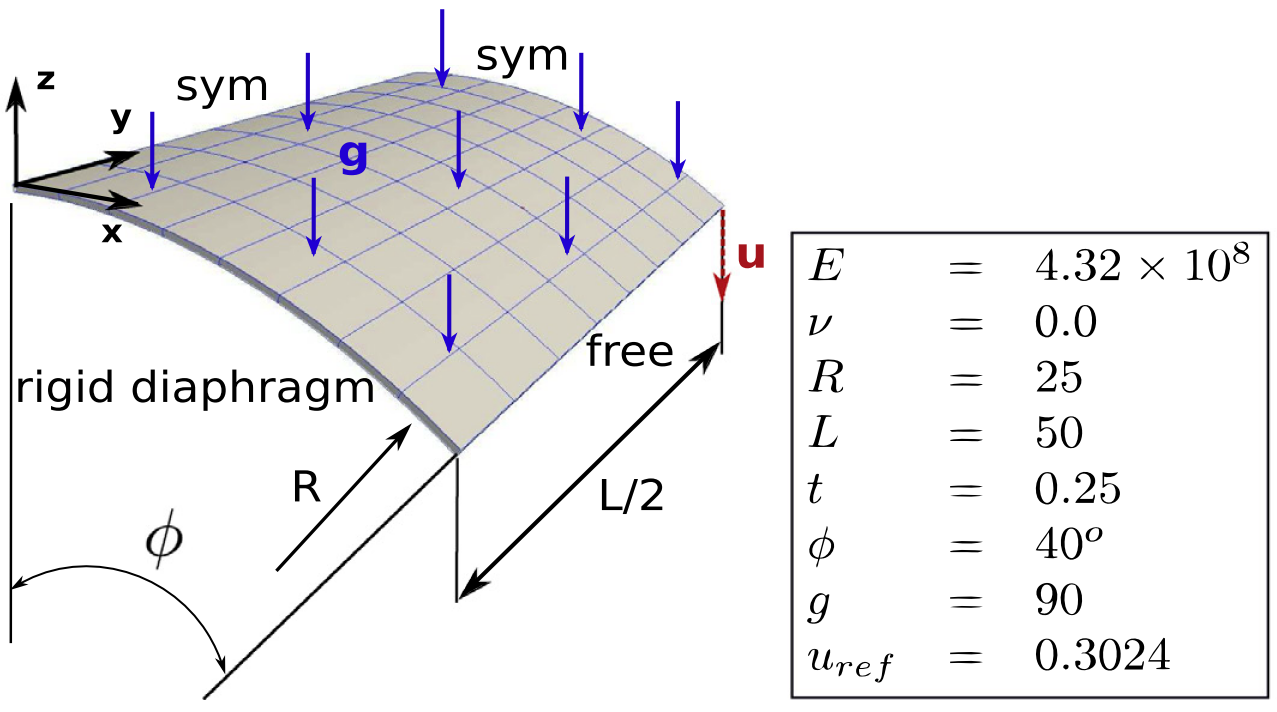
\includegraphics[width=0.40\textwidth]{images/scordelisroof.png}
%	\caption{Definition of the Scordelis-Lo roof benchmark\cite{Bou13}}
%\end{wrapfigure}

The first problem of the shell obstacle course is the Scordelis-Lo roof, which is part of a cylindrical shell fixed by rigid diaphragms at it's axial ends. The loading is a pseudo-gravity distributed load that has a magnitude of 90. Due to symmetry, only a quarter of the shell is modelled. The key result is the vertical displacement of the lateral side at the midpoint, denoted by $\textcolor{red}{u}$ in the following diagram. The reference value is $u_{ref} = 0.3024$.
 
  \begin{figure}[H]
 	\centering
 	\def\svgwidth{\columnwidth}
 	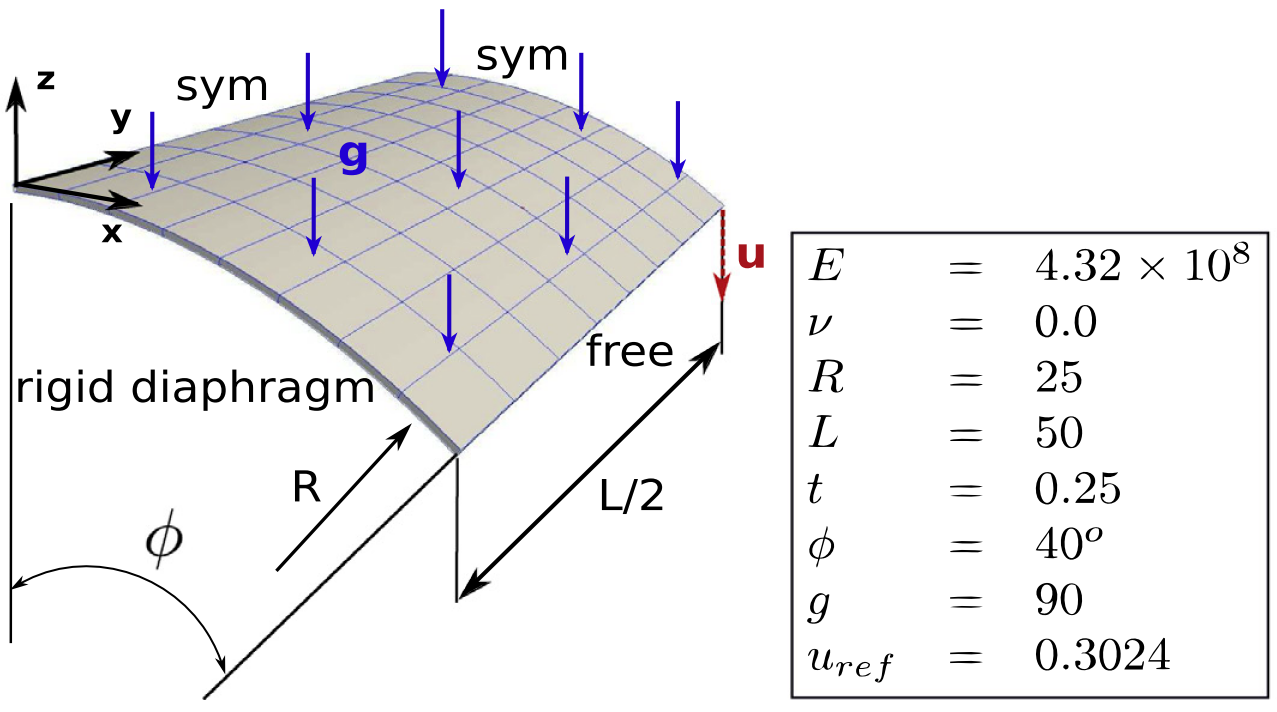
\includegraphics[width=7.3cm]{images/scordelisroof.png}
 	\caption{Definition of the Scordelis-Lo roof benchmark\cite{Bou13}}
 \end{figure}
 
\begin{figure}[H]
	\subfloat[Quadrilateral element convergence for the Scordelis-Lo roof benchmark]
	{\label{ref_label2}
		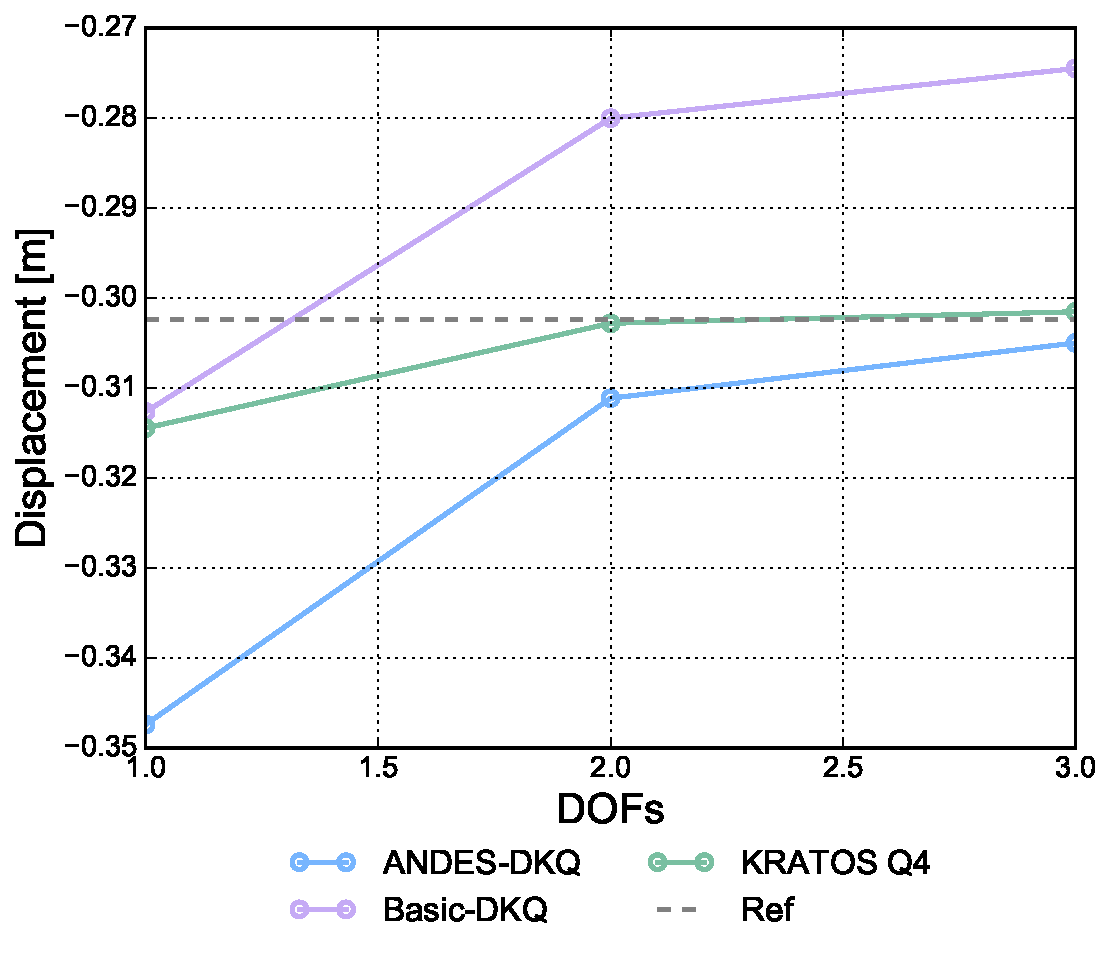
\includegraphics[width=7.3cm]
		{scordelis_structured_quad_results.pdf}}
	\subfloat[Triangle element convergence for the Scordelis-Lo roof benchmark]
	{\label{ref_label2}
		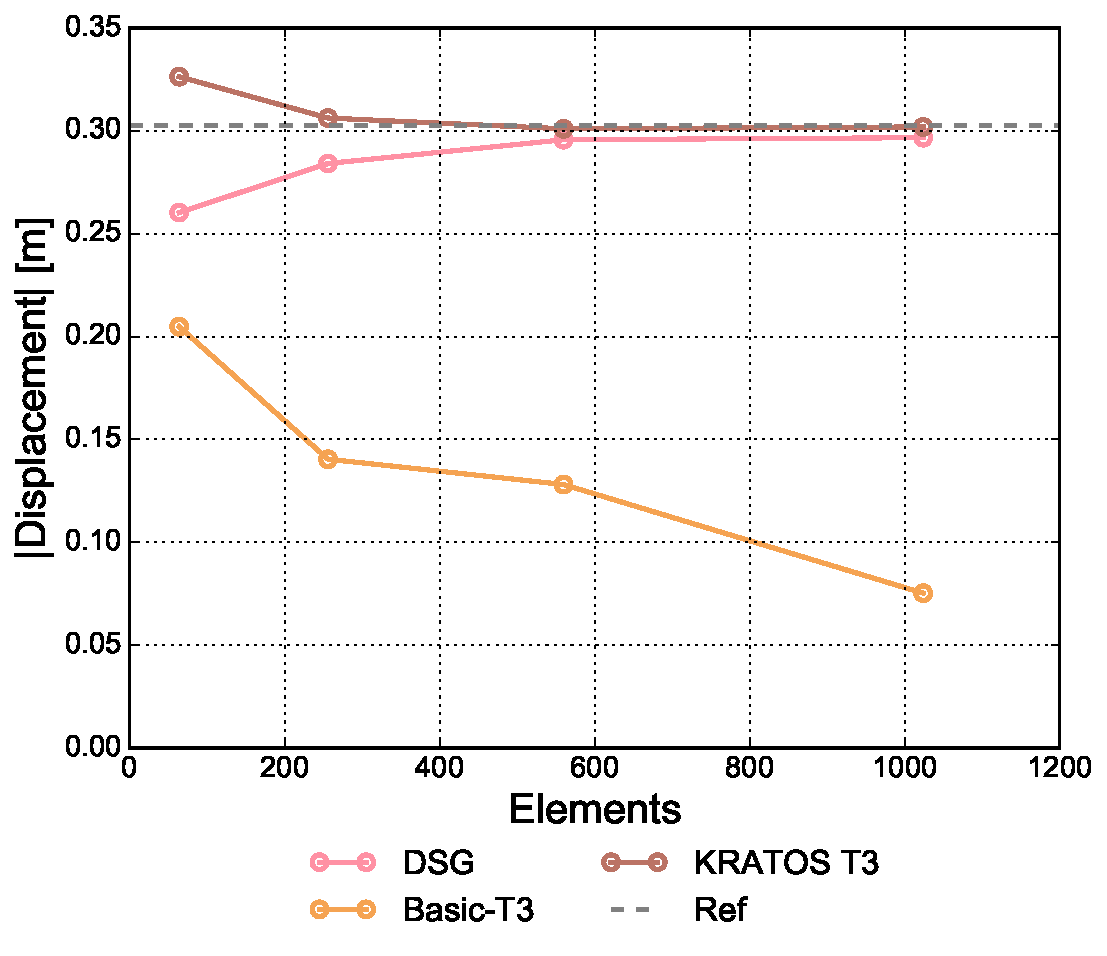
\includegraphics[width=7.3cm]
		{scordelis_structured_tri_results.pdf}}
	\caption{\label{ref_label_overall}Scordelis-Lo roof benchmark results}
\end{figure}

The convergence graphs above indicate the ANDES-DKQ and DSG elements agree to the reference solution. Conversely, the Basic-T3 element shows very poor performance. Given that the Basic-DKQ performs well (which is immune to transverse shear locking), it's suspected that transverse shear locking is crippling the Basic-T3 element, while the DSG element technology effectively mitigates this for the DSG element. 
\newpage
\subsection{Pinched cylinder}
%
%\begin{wrapfigure}{r}{0.45\textwidth}
%	\centering
%	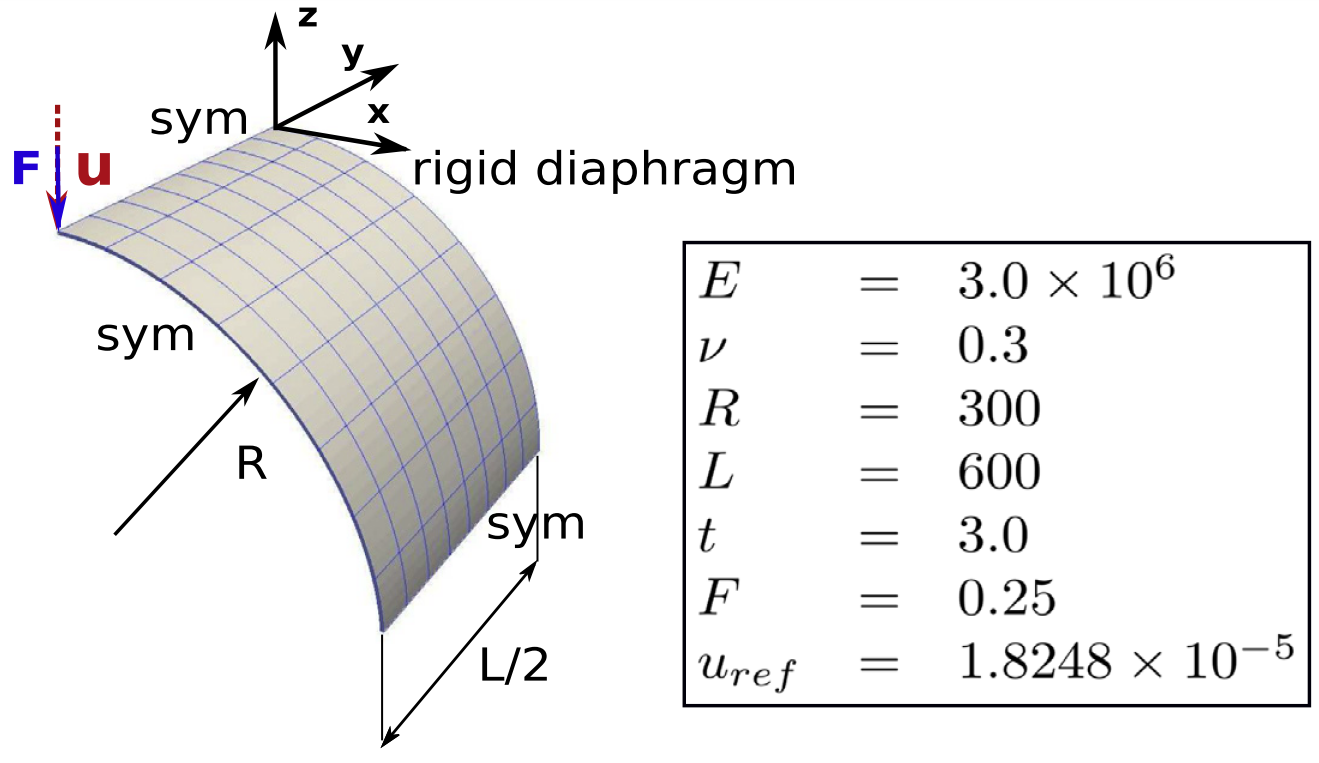
\includegraphics[width=0.4\textwidth]{images/pinchedcylinder.png}
%	\caption{Definition of the pinched cylinder benchmark\cite{Bou13}}
%\end{wrapfigure}

The second problem of the shell obstacle course is the pinched cylinder, which considers a cylindrical shell fixed by rigid diaphragms at it's axial ends. The loading consists of two opposing compressive point loads at the centre of the shell. Due to symmetry only an eighth of the shell is modelled. The key result is the vertical displacement under the point load, denoted by $\textcolor{red}{u}$ in the following diagram. The reference value is $u_{ref} =  1.8248\ \times\ 10^{-5}$. 
 
 \begin{figure}[H]
 	\centering
 	\def\svgwidth{\columnwidth}
 	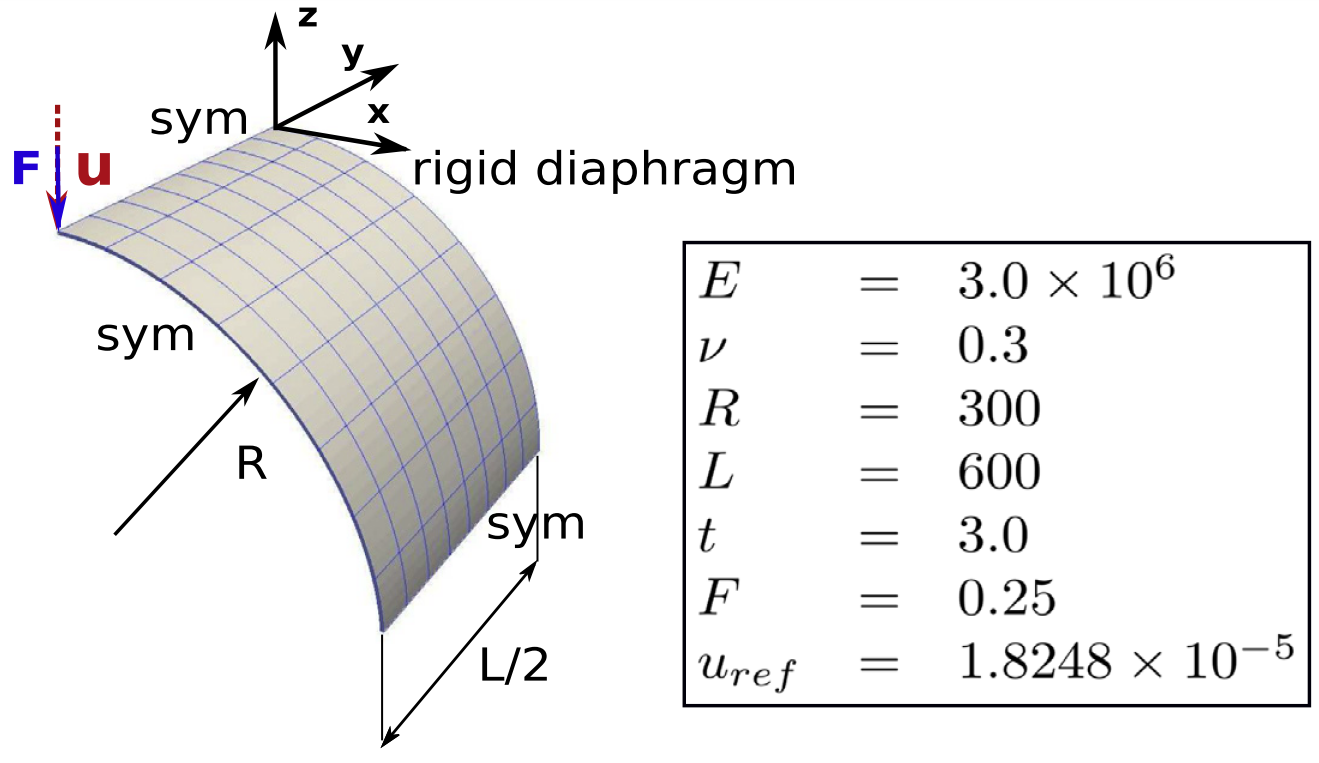
\includegraphics[width=7.3cm]{images/pinchedcylinder.png}
 	\caption{Definition of the pinched cylinder benchmark\cite{Bou13}}
 \end{figure}
 
\begin{figure}[H]
	\subfloat[Quadrilateral element convergence for the pinched cylinder benchmark]
	{\label{ref_label2}
		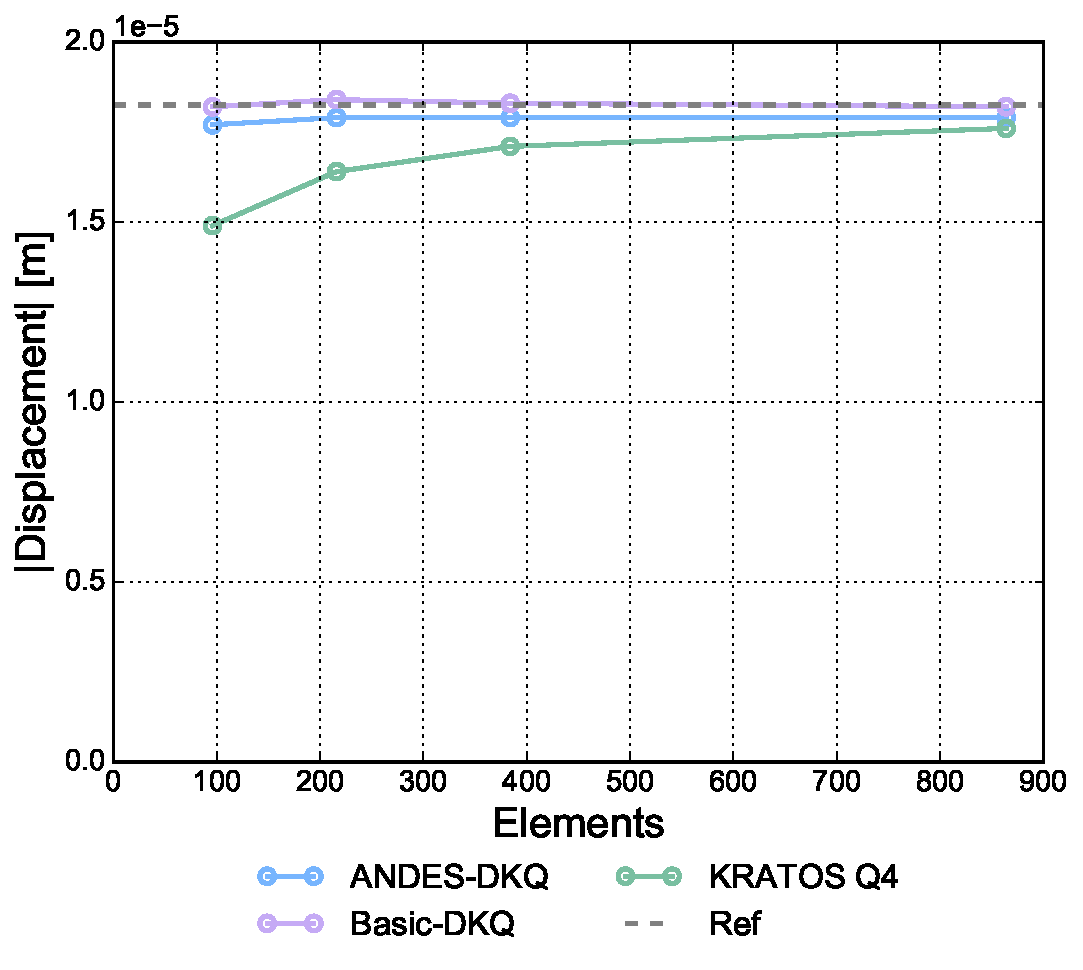
\includegraphics[width=7.3cm]
		{pinched_cyl_structured_quad_results.pdf}}
	\subfloat[Triangle element convergence for the pinched cylinder benchmark]
	{\label{ref_label2}
		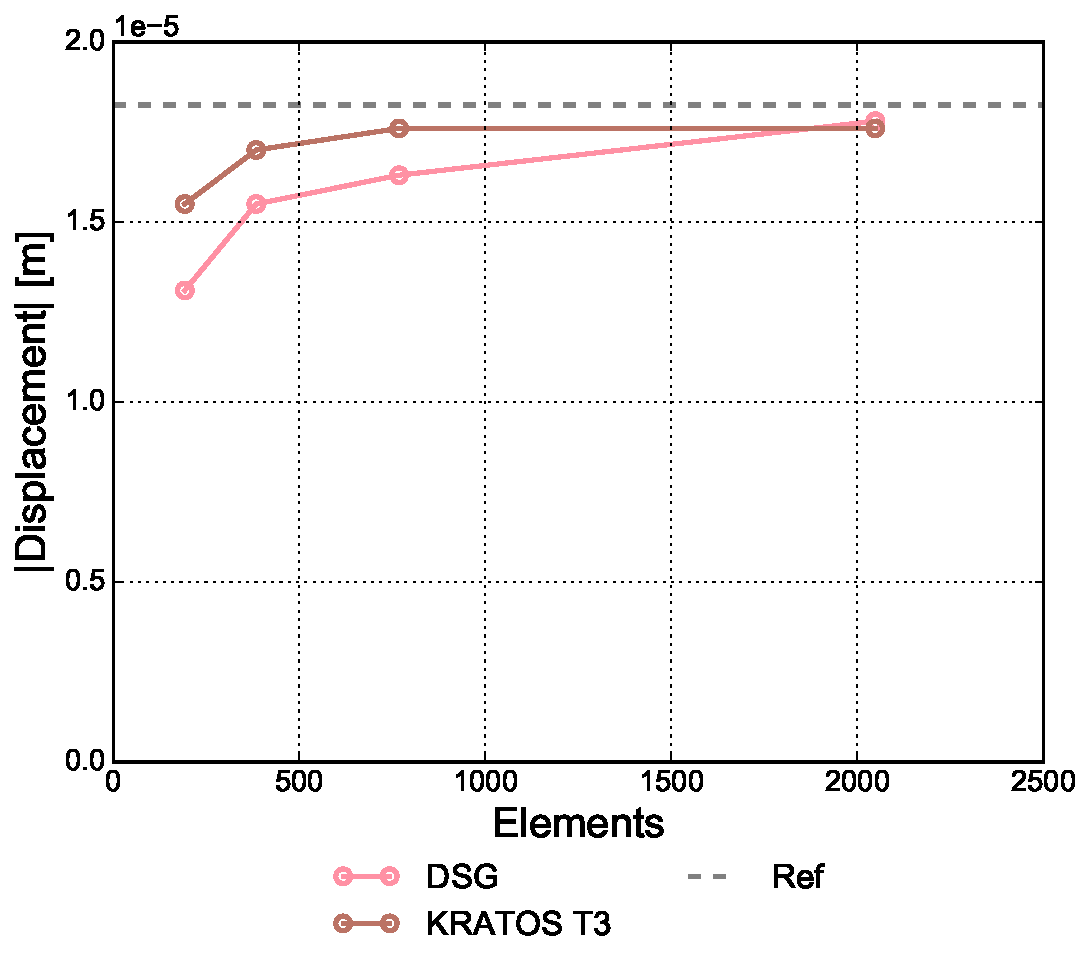
\includegraphics[width=7.3cm]
		{pinched_cyl_structured_tri_results.pdf}}
	\caption{\label{ref_label_overall}Pinched cylinder benchmark results}
\end{figure}

 The good performance of both the ANDES-DKQ and DSG elements is demonstrated in the convergence graphs above. The Basic-T3 results were in the order of $1\times10^{-3}$ (roughly 100 times greater than the reference solution) and were omitted from the graph for clarity of scale. Once again, it is clear that the computationally inexpensive DSG element technology drastically improves performance from the un-enhanced Basic-T3 to the DSG element.
\newpage
\subsection{Pinched hemisphere}
%
%\begin{wrapfigure}{r}{0.45\textwidth}
%	\centering
%	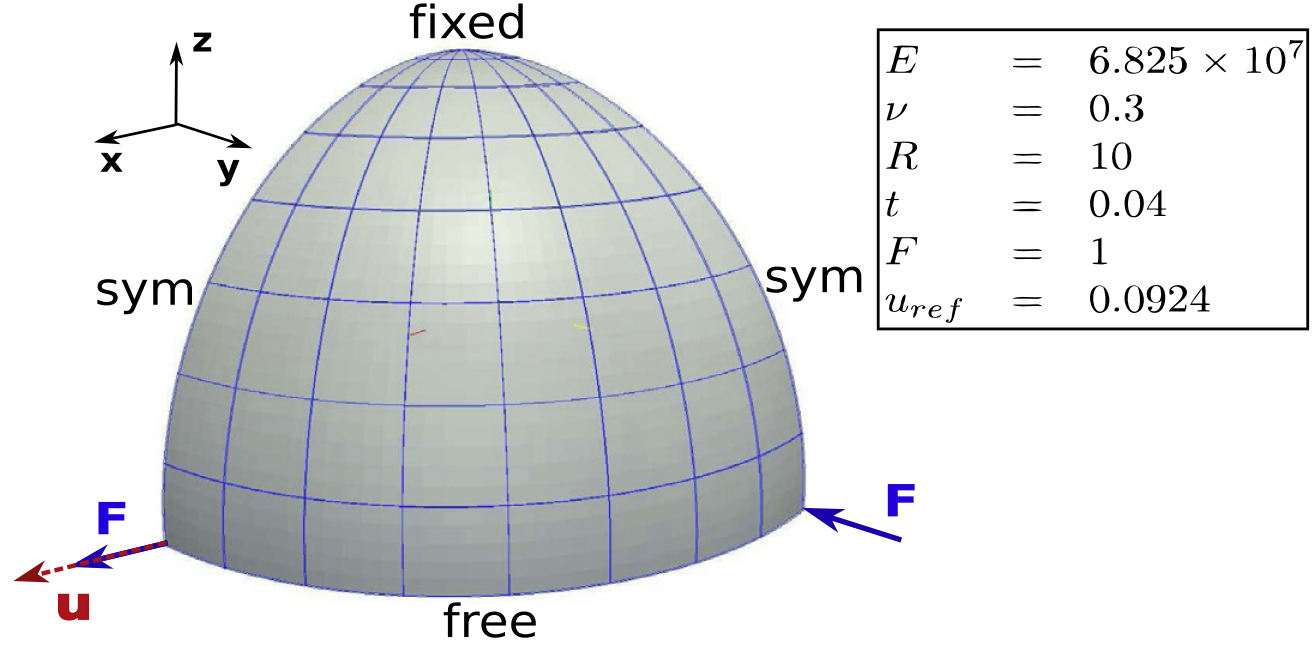
\includegraphics[width=0.4\textwidth]{images/pinchedhemisphere.png}
%	\caption{Definition of the pinched hemisphere benchmark \cite{Bou13}}
%\end{wrapfigure}

The last test in the shell obstacle course is the pinched hemisphere, which considers a hemispherical shell loaded with opposing point loads along it's equator. Due to symmetry only a quarter of the shell is modelled. The key result is the 'x' displacement along one of the point loads, denoted by $\textcolor{red}{u}$ in the following diagram. The reference value is $u_{ref} =  0.0924$. 

\begin{figure}[H]
	\centering
	\def\svgwidth{\columnwidth}
	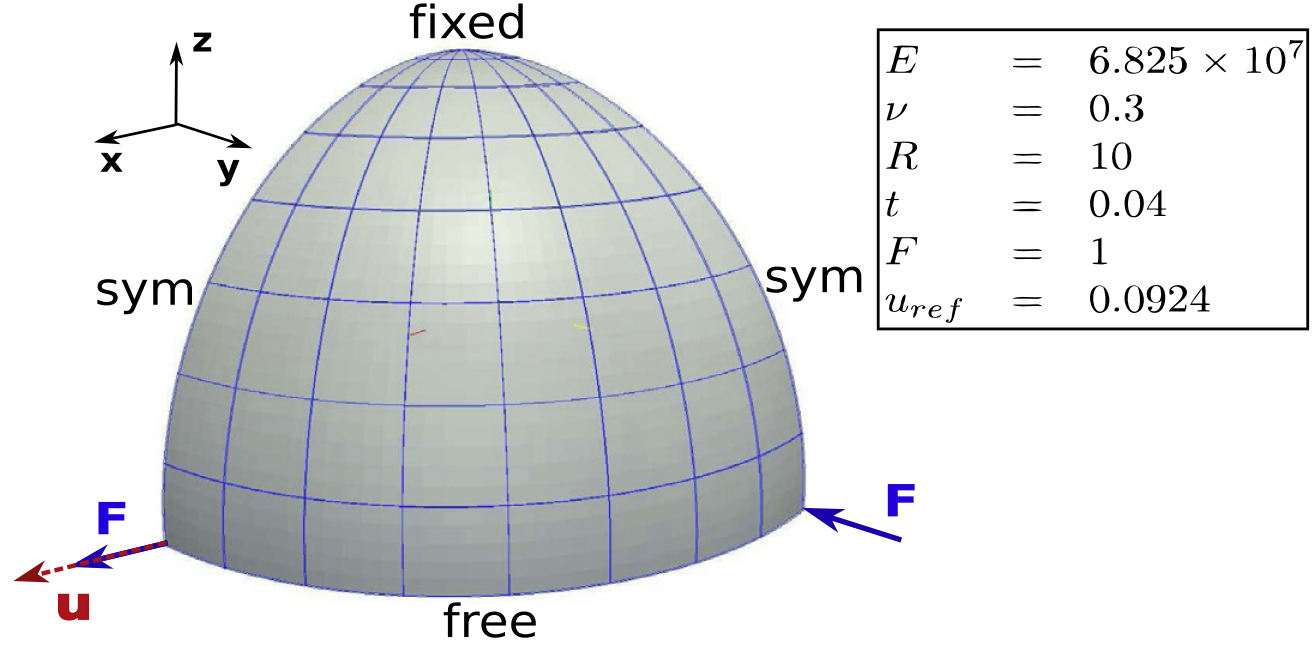
\includegraphics[width=7.3cm]{images/pinchedhemisphere.png}
	\caption{Definition of the pinched hemisphere benchmark \cite{Bou13}}
\end{figure}

\begin{figure}[H]
	\subfloat[Quadrilateral element convergence for the pinched hemisphere benchmark]
	{\label{ref_label2}
		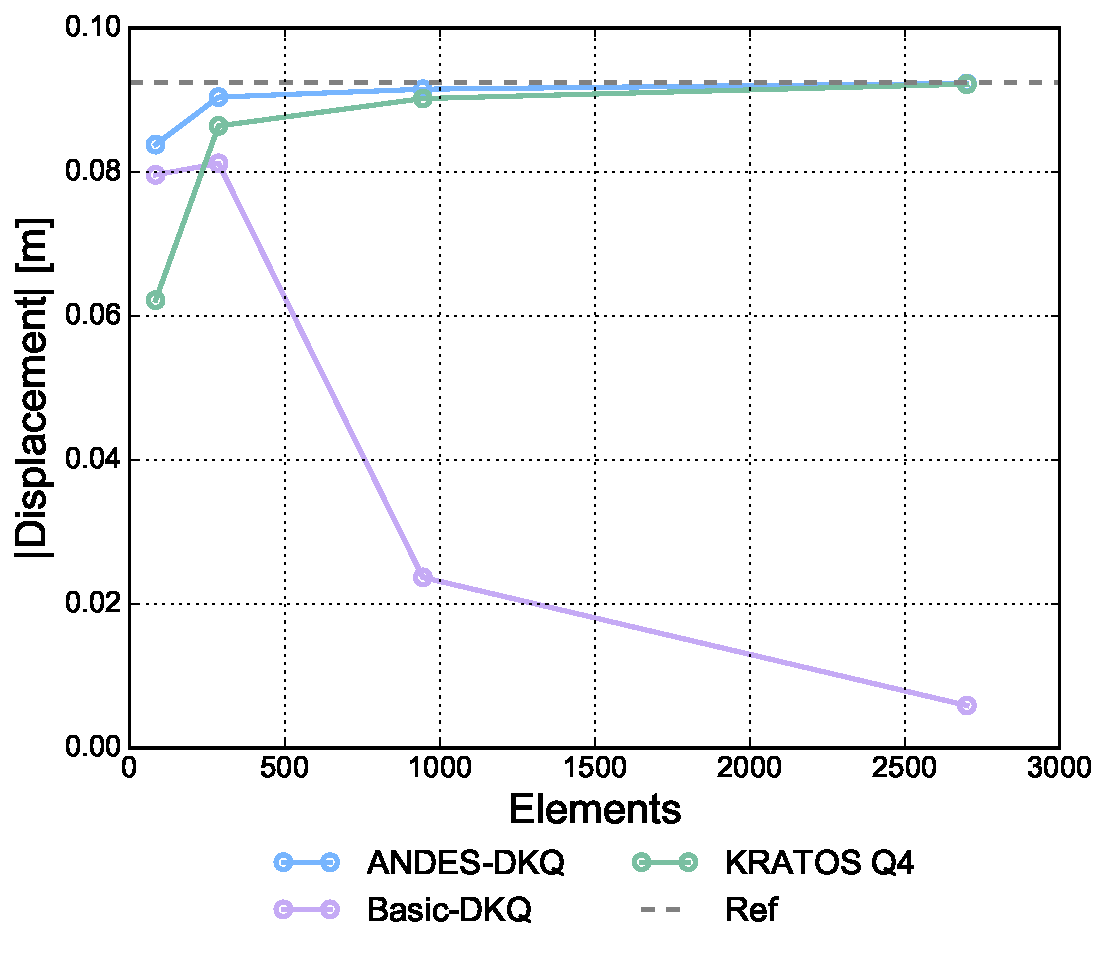
\includegraphics[width=7.3cm]
		{pinched_hemi_quad_results.pdf}}
	\subfloat[Triangle element convergence for the pinched hemisphere benchmark]
	{\label{ref_label2}
		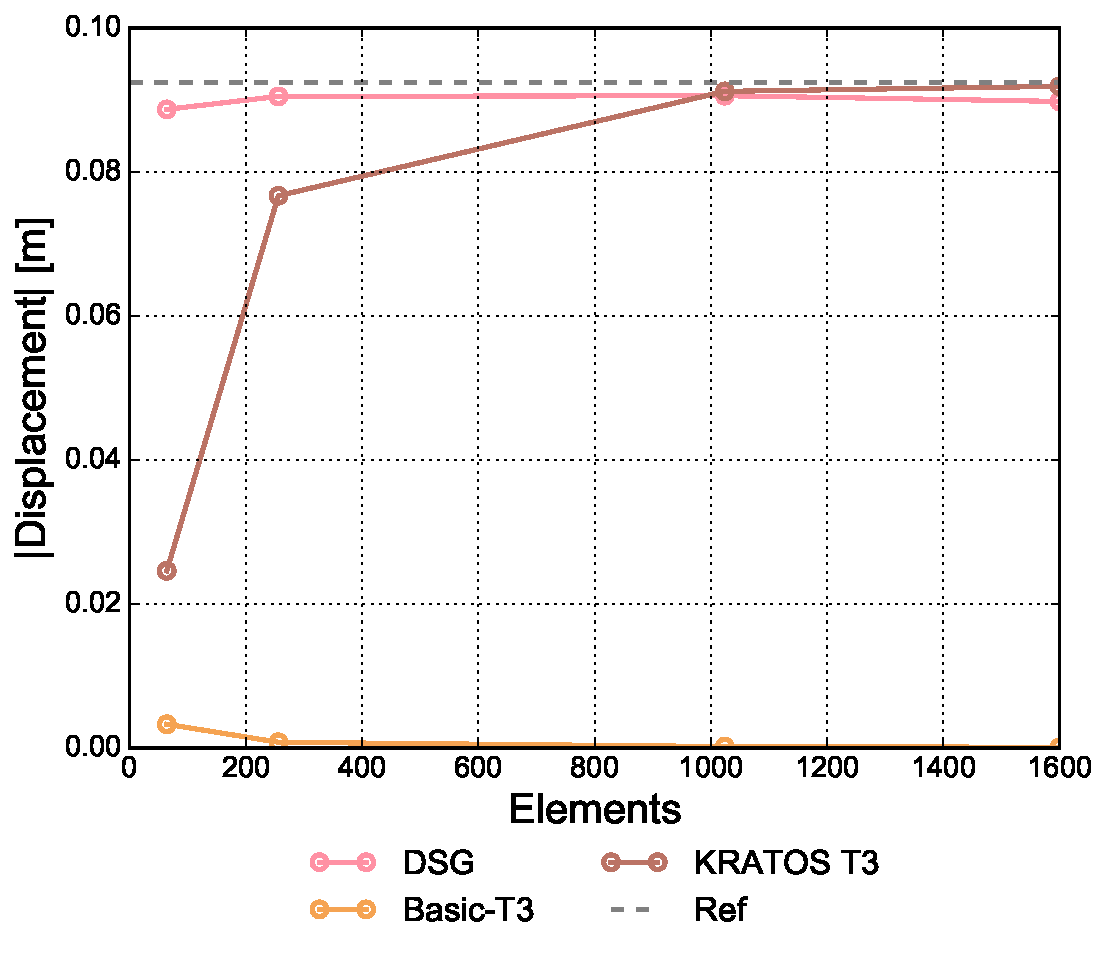
\includegraphics[width=7.3cm]
		{pinched_hemi_tri_results.pdf}}
	\caption{\label{ref_label_overall}Pinched hemisphere benchmark results}
\end{figure}

The ANDES-DKQ and DSG elements both perform well in the final statics test, as per the convergence graphs above. It is observed that the Basic-DKQ element appears to exhibit membrane locking corresponding to the high double curvature of the problem ($R_1=R_2 = 10$) compared to the Scordelis-Lo roof ($R_1= 10,\ R_2 = \infty$) and the pinched cylinder ($R_1= 300,\ R_2 = \infty$). The ANDES element technology clearly prevents this deleterious effect. The poor performance of the Basic-T3 element compared to the DSG element once again highlights the effectiveness of the DSG element technology in preventing transverse shear locking.
\newpage
\section{Geometically non-linear tests}

Large rotations and displacements mark the departure from geometrically linear to non-linear analyses, however, the assumption of small strains is still maintained. The extension of the elements to geometrically non-linear problems is handled by employing an existing Kratos class which provides co-rotational transformations for shells. At each increment in the non-linear solution, the large displacements and rotations of each element is mapped by rigid body translations and rotations, thus limiting the strains experienced by the element to reasonably small magnitudes. The performance of the element in geometrically non-linear problems is considered with two benchmarks.

\subsection{Hinged cylindrical roof}
\label{validation:hinged cyl roof}
The first geometrically non-linear benchmark is the snap-through of a hinged cylindrical roof under a central point load $P_{max} = 3000$ \cite{Sze2004}. As per the diagram below, the roof geometry is defined with the parameters: $L = 254,\ R = 2540,\ \theta=0.1\ rad$ and $h = 12.7$. The material is defined with a Young's modulus $E = 3102.75$ and Poisson's ratio of $\nu = 0.3$.

 
\begin{figure}[H]
	%\centering
	\subfloat[Hinged cylindrical roof definition \cite{Sze2004}]
	{\label{ref_label1}
		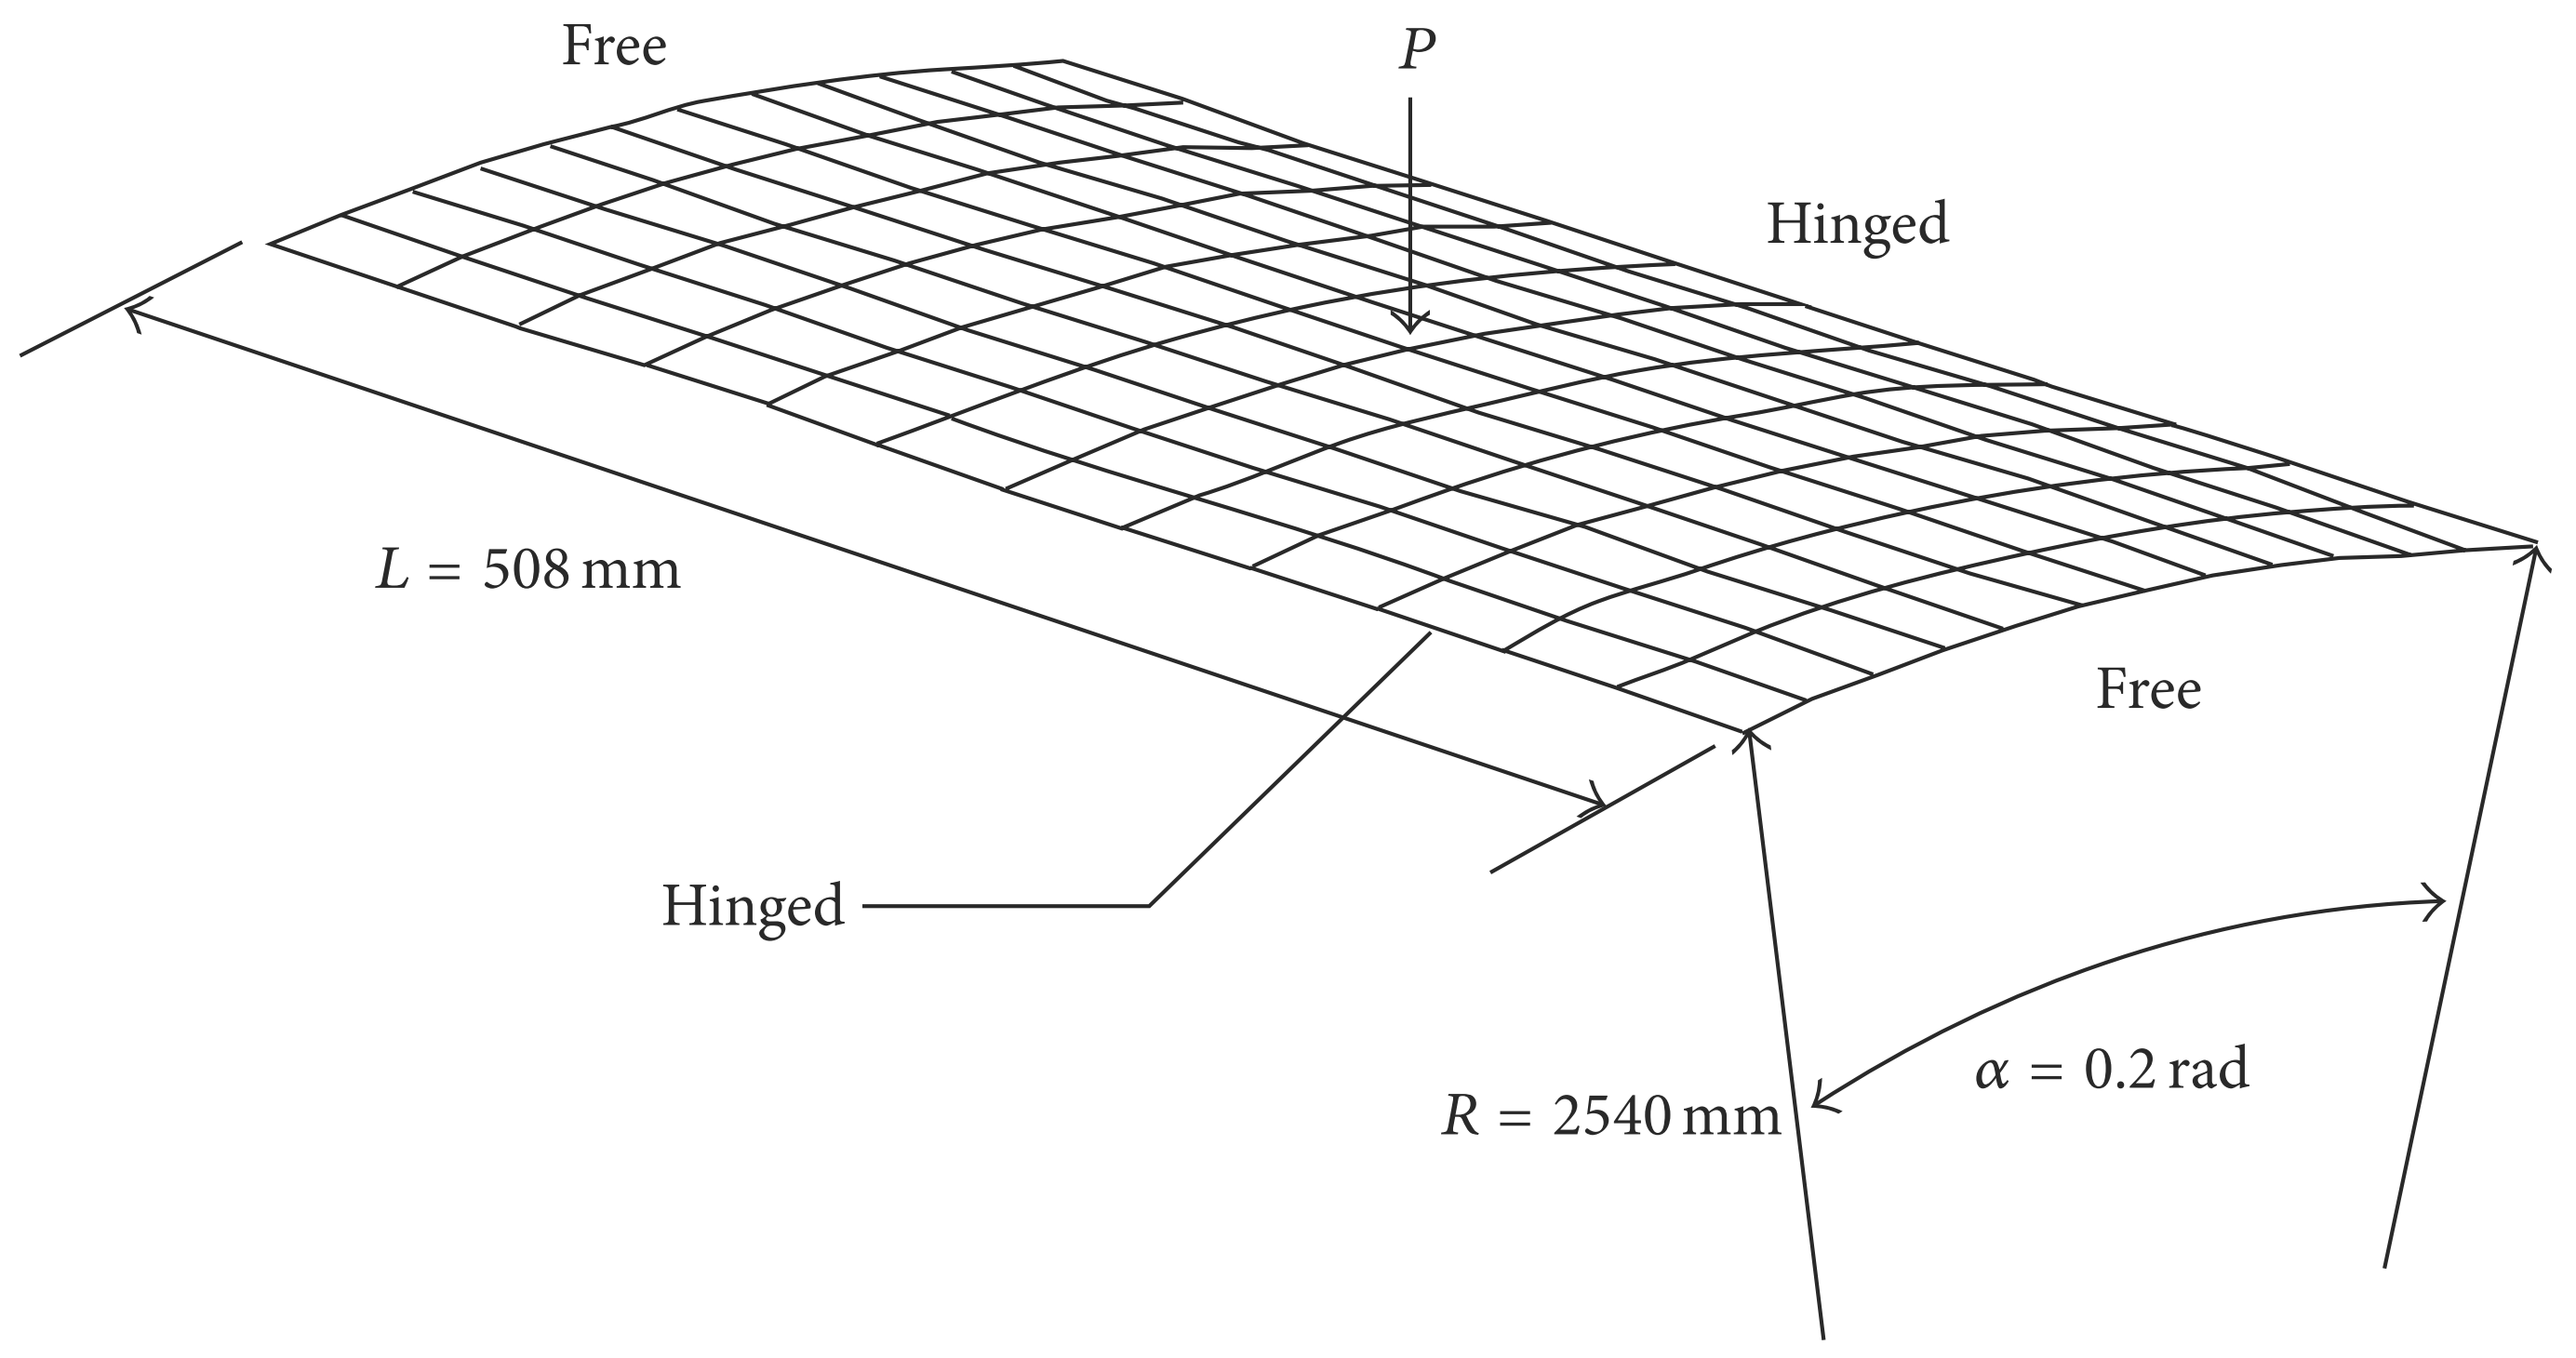
\includegraphics[width=7.3cm]
		{images/hinged_cylindrical_roof.png}}
	\subfloat[Load-displacement curve of hinged cylindrical roof]
	{\label{ref_label2}
		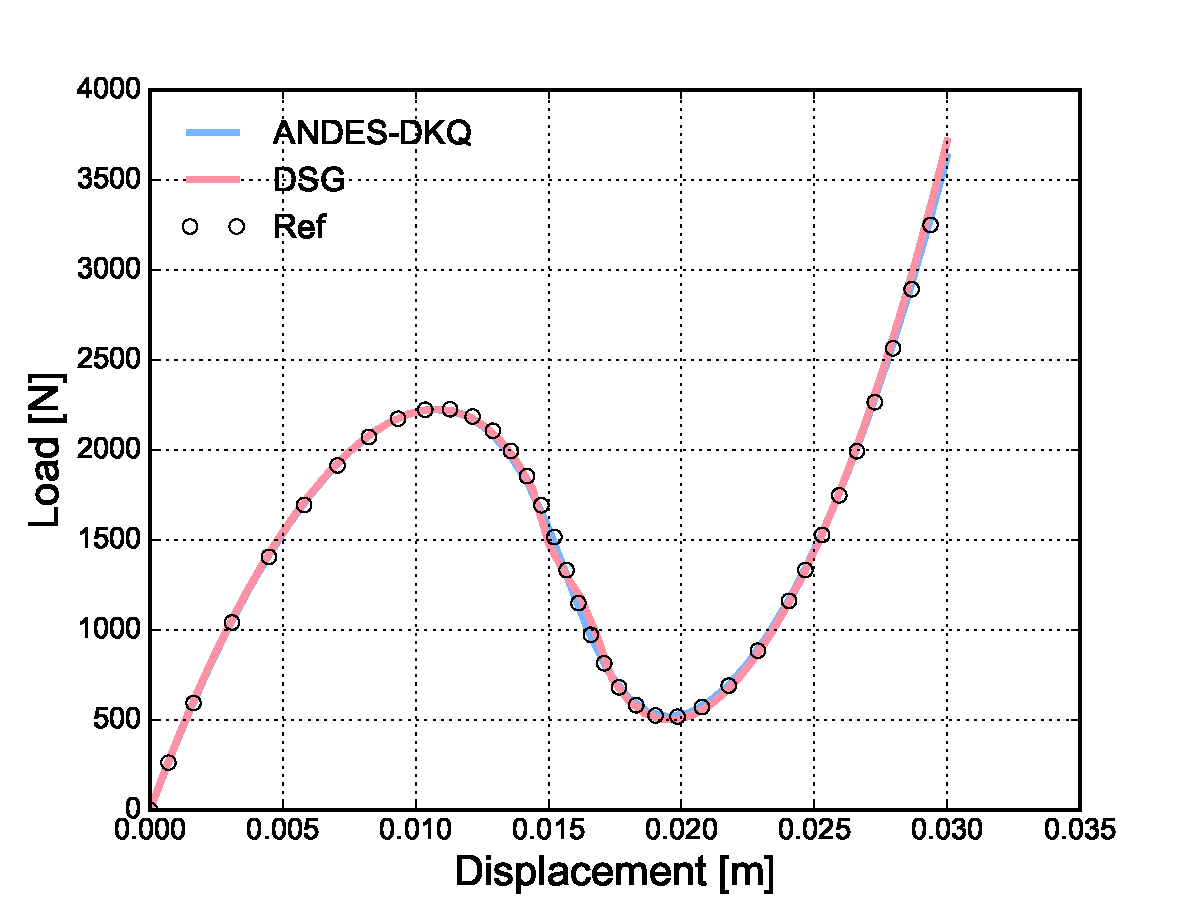
\includegraphics[width=7.3cm]
		{Load_displacement_curve_hinged_cylindrical_roof.pdf}}
	\caption{\label{ref_label_overall}Hinged cylindrical roof benchmark}
\end{figure}

 
The load displacement curve plots the equilibrium path for the ANDES-DKQ and DSG elements against the reference path from \cite{Sze2004}. The full equilibrium path isn't resolved because Kratos only has a load control non-linear solution method implemented, translating to the restriction of only resolving monotonically increasing paths. Regardless, both elements clearly follow the initial path, and then rejoin the reference solution to correctly resolve the structure in it's snapped-through state.

\newpage
\subsection{Open cylinder pull-out}

The second geometrically non-linear benchmark is the pull-out of an open cylinder with a load $P_{max} = 40\ 000$. The geometry of the cylinder is $L= 10.35,\ R = 4.953$ and $h = 0.094$ while the linear elastic material is characterised by $E = 10.5\times10^6$ and $\nu = 0.3125$. The measured displacement is the vertical deformation $u_z$ at the point of load application.

 
\begin{figure}[H]
	%\centering
	\subfloat[Open cylinder pullout definition \cite{Sze2004}]
	{\label{ref_label1}
		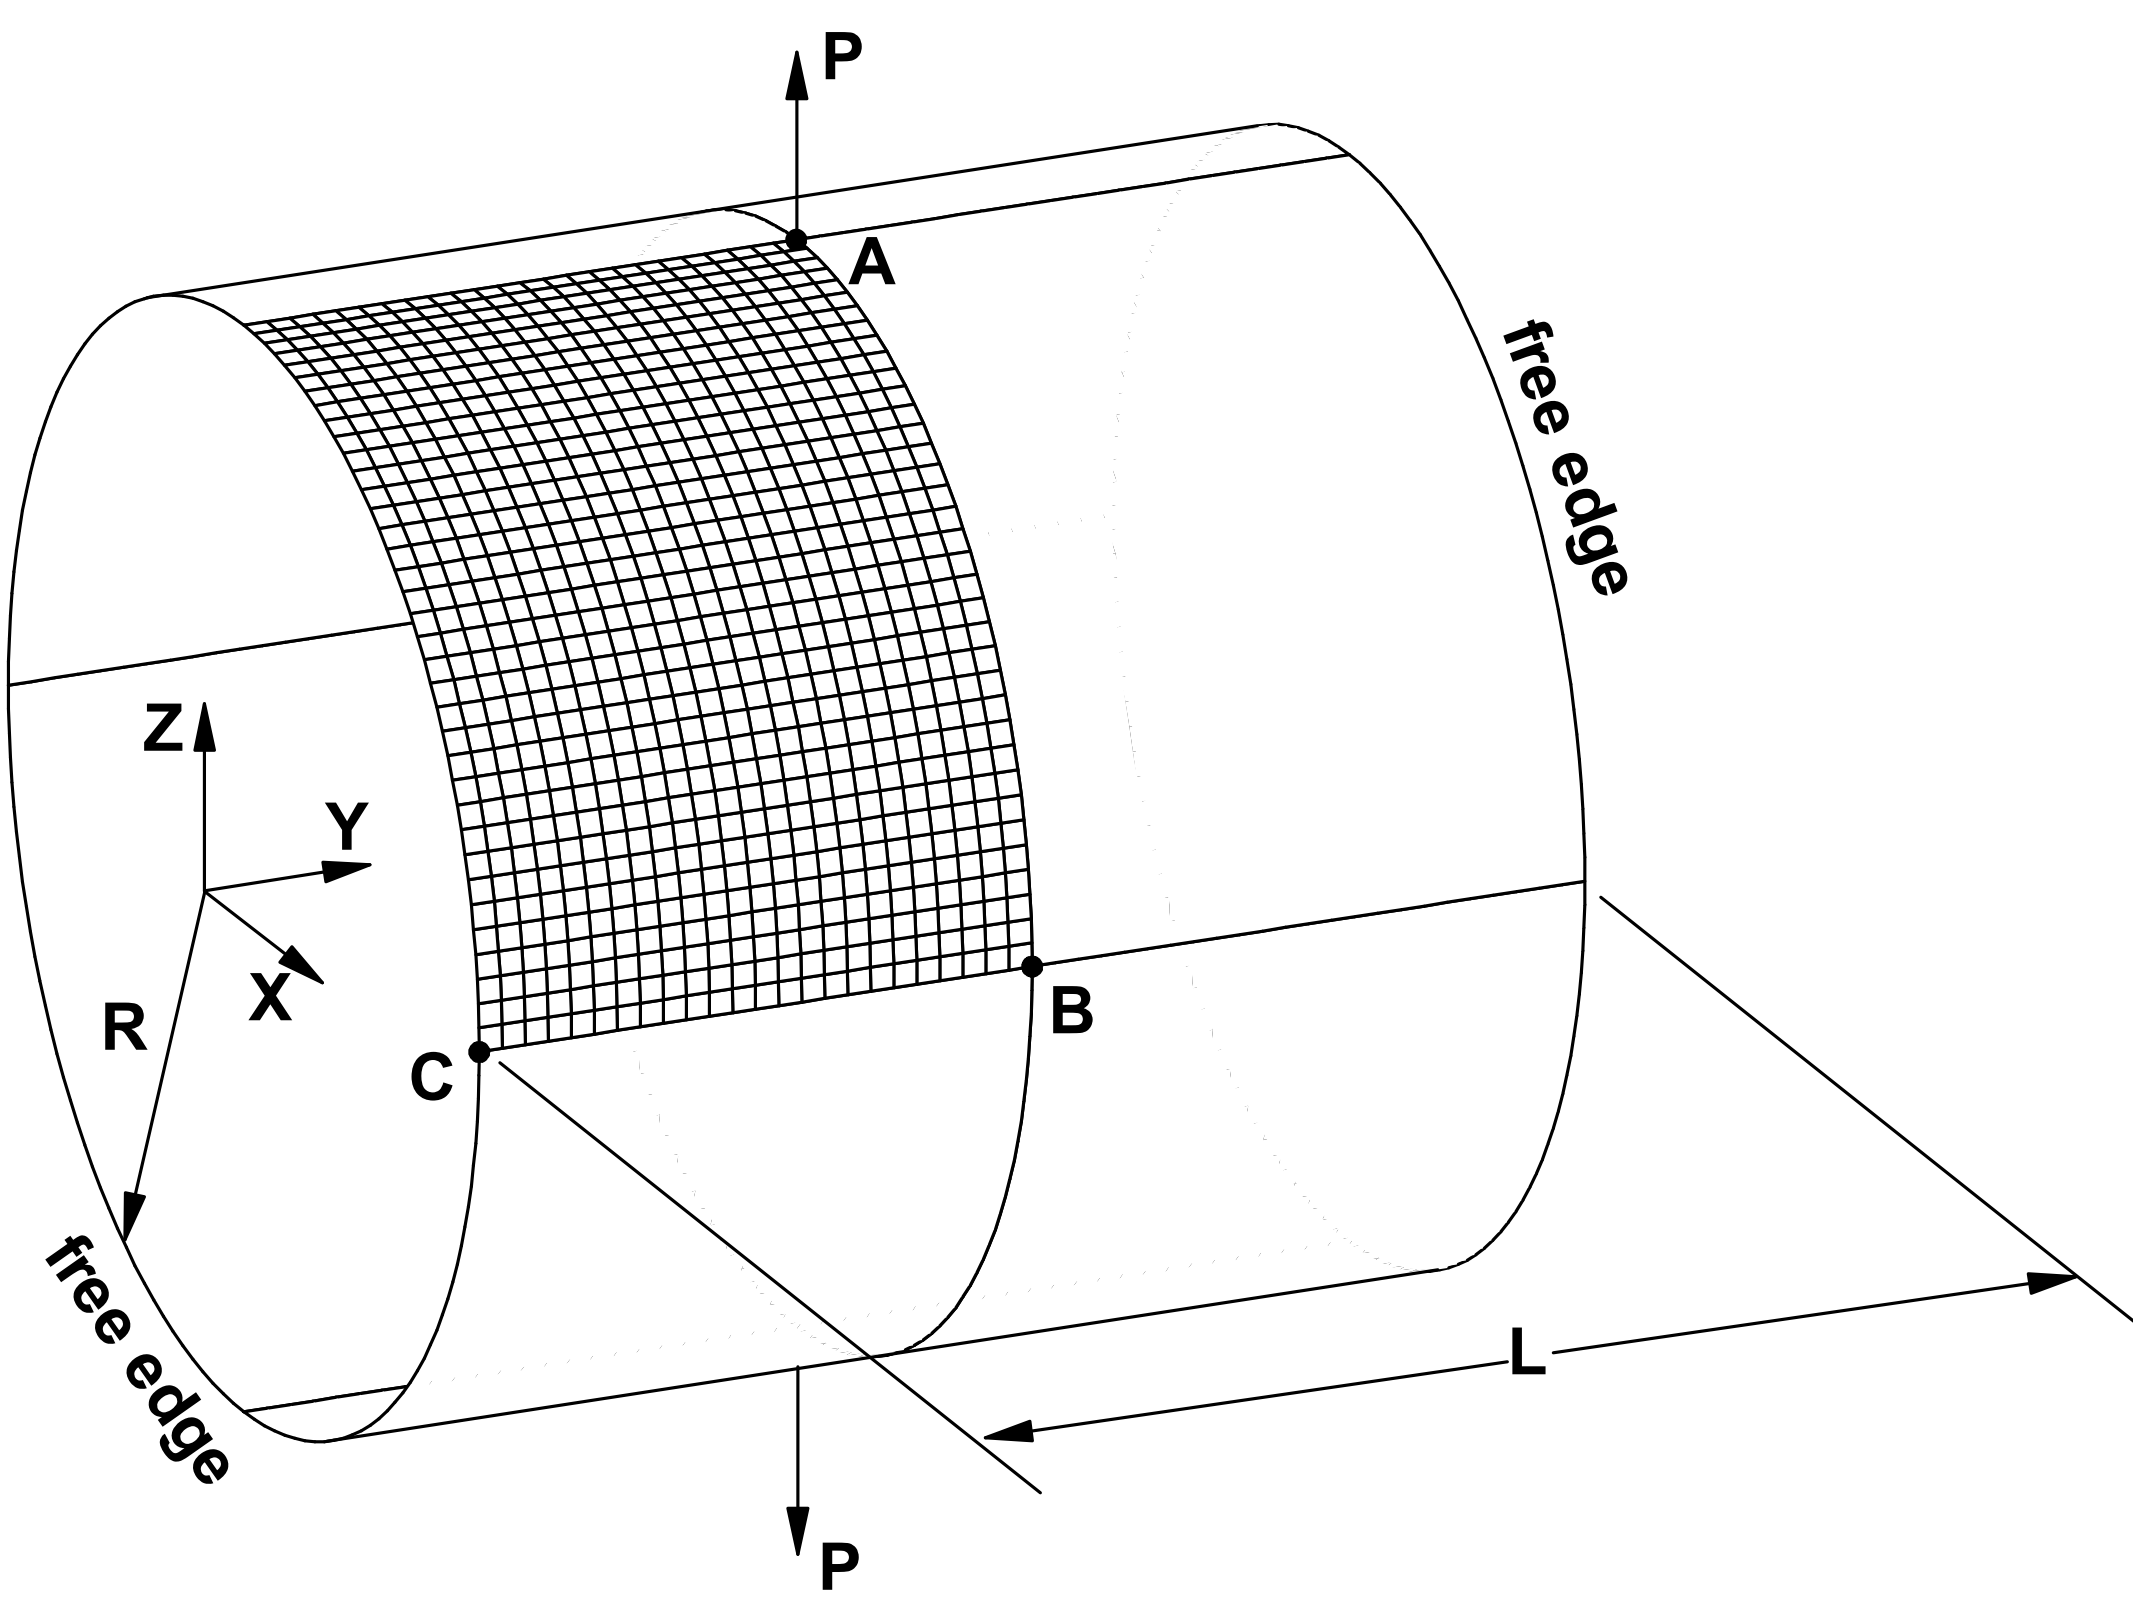
\includegraphics[width=7.3cm]
		{images/opencylinderpullout.png}}
	\subfloat[Load-displacement curve of open cylinder pullout]
	{\label{ref_label2}
		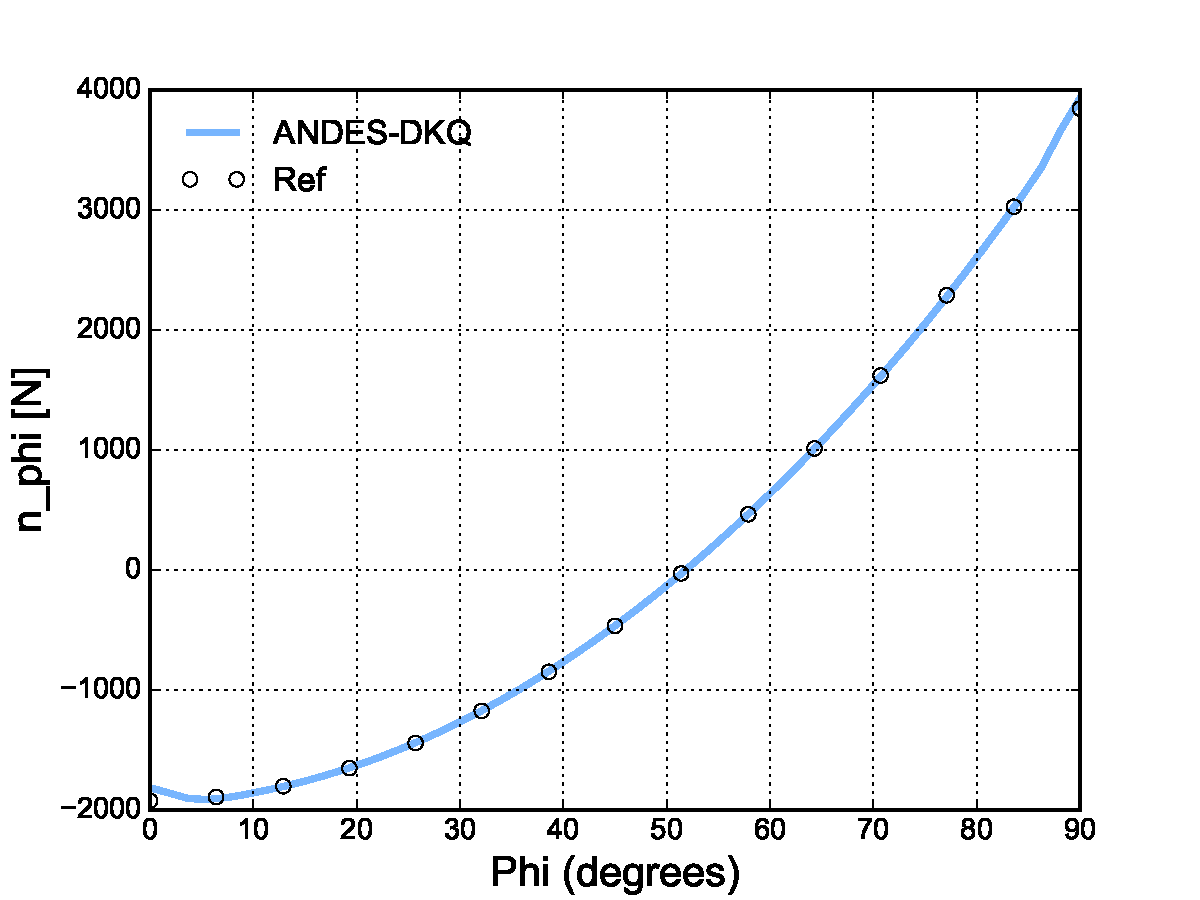
\includegraphics[width=7.3cm]
		{Load_displacement_curve_open_cylinder_pullout.pdf}}
	\caption{\label{ref_label_overall}Open cylinder pullout benchmark}
\end{figure}

 The load-displacement curve above plots the equilibrium path for the ANDES-DKQ and DSG elements against the reference solution \cite{Sze2004}. Although both elements closely follow the reference path, the ANDES-DKQ performs better in this test than the DSG element. Despite this, the error of the DSG element at maximum load is still only 1.7\%.

\section{Dynamic tests}

Dynamic problems introduce inertial effects into the array of phenomena analysed. Combined with the aforementioned co-rotational formulation, it is possible to accurately resolve bodies undergoing large movements over time.

\subsection{Shell pendulum}
\label{validation:shell pendulum}
The first dynamic benchmark is a simple shell pendulum allowed to freely rotate along one hinged edge. The initial horizontal configuration of the $1m\times1m\times0.1m$ thick square plate is subject to gravity $g = 9.8\ m/s^2$ acting in the vertical $Z$ direction. The material of the plate is described by $E = 1\times 10^9 Pa,\ \nu = 0.0$ and $\rho = 7850 kg/m^3$. The key result is the vertical displacement component of the free corner node as drawn below.

\begin{figure}[H]
	\centering
	\def\svgwidth{\columnwidth}
	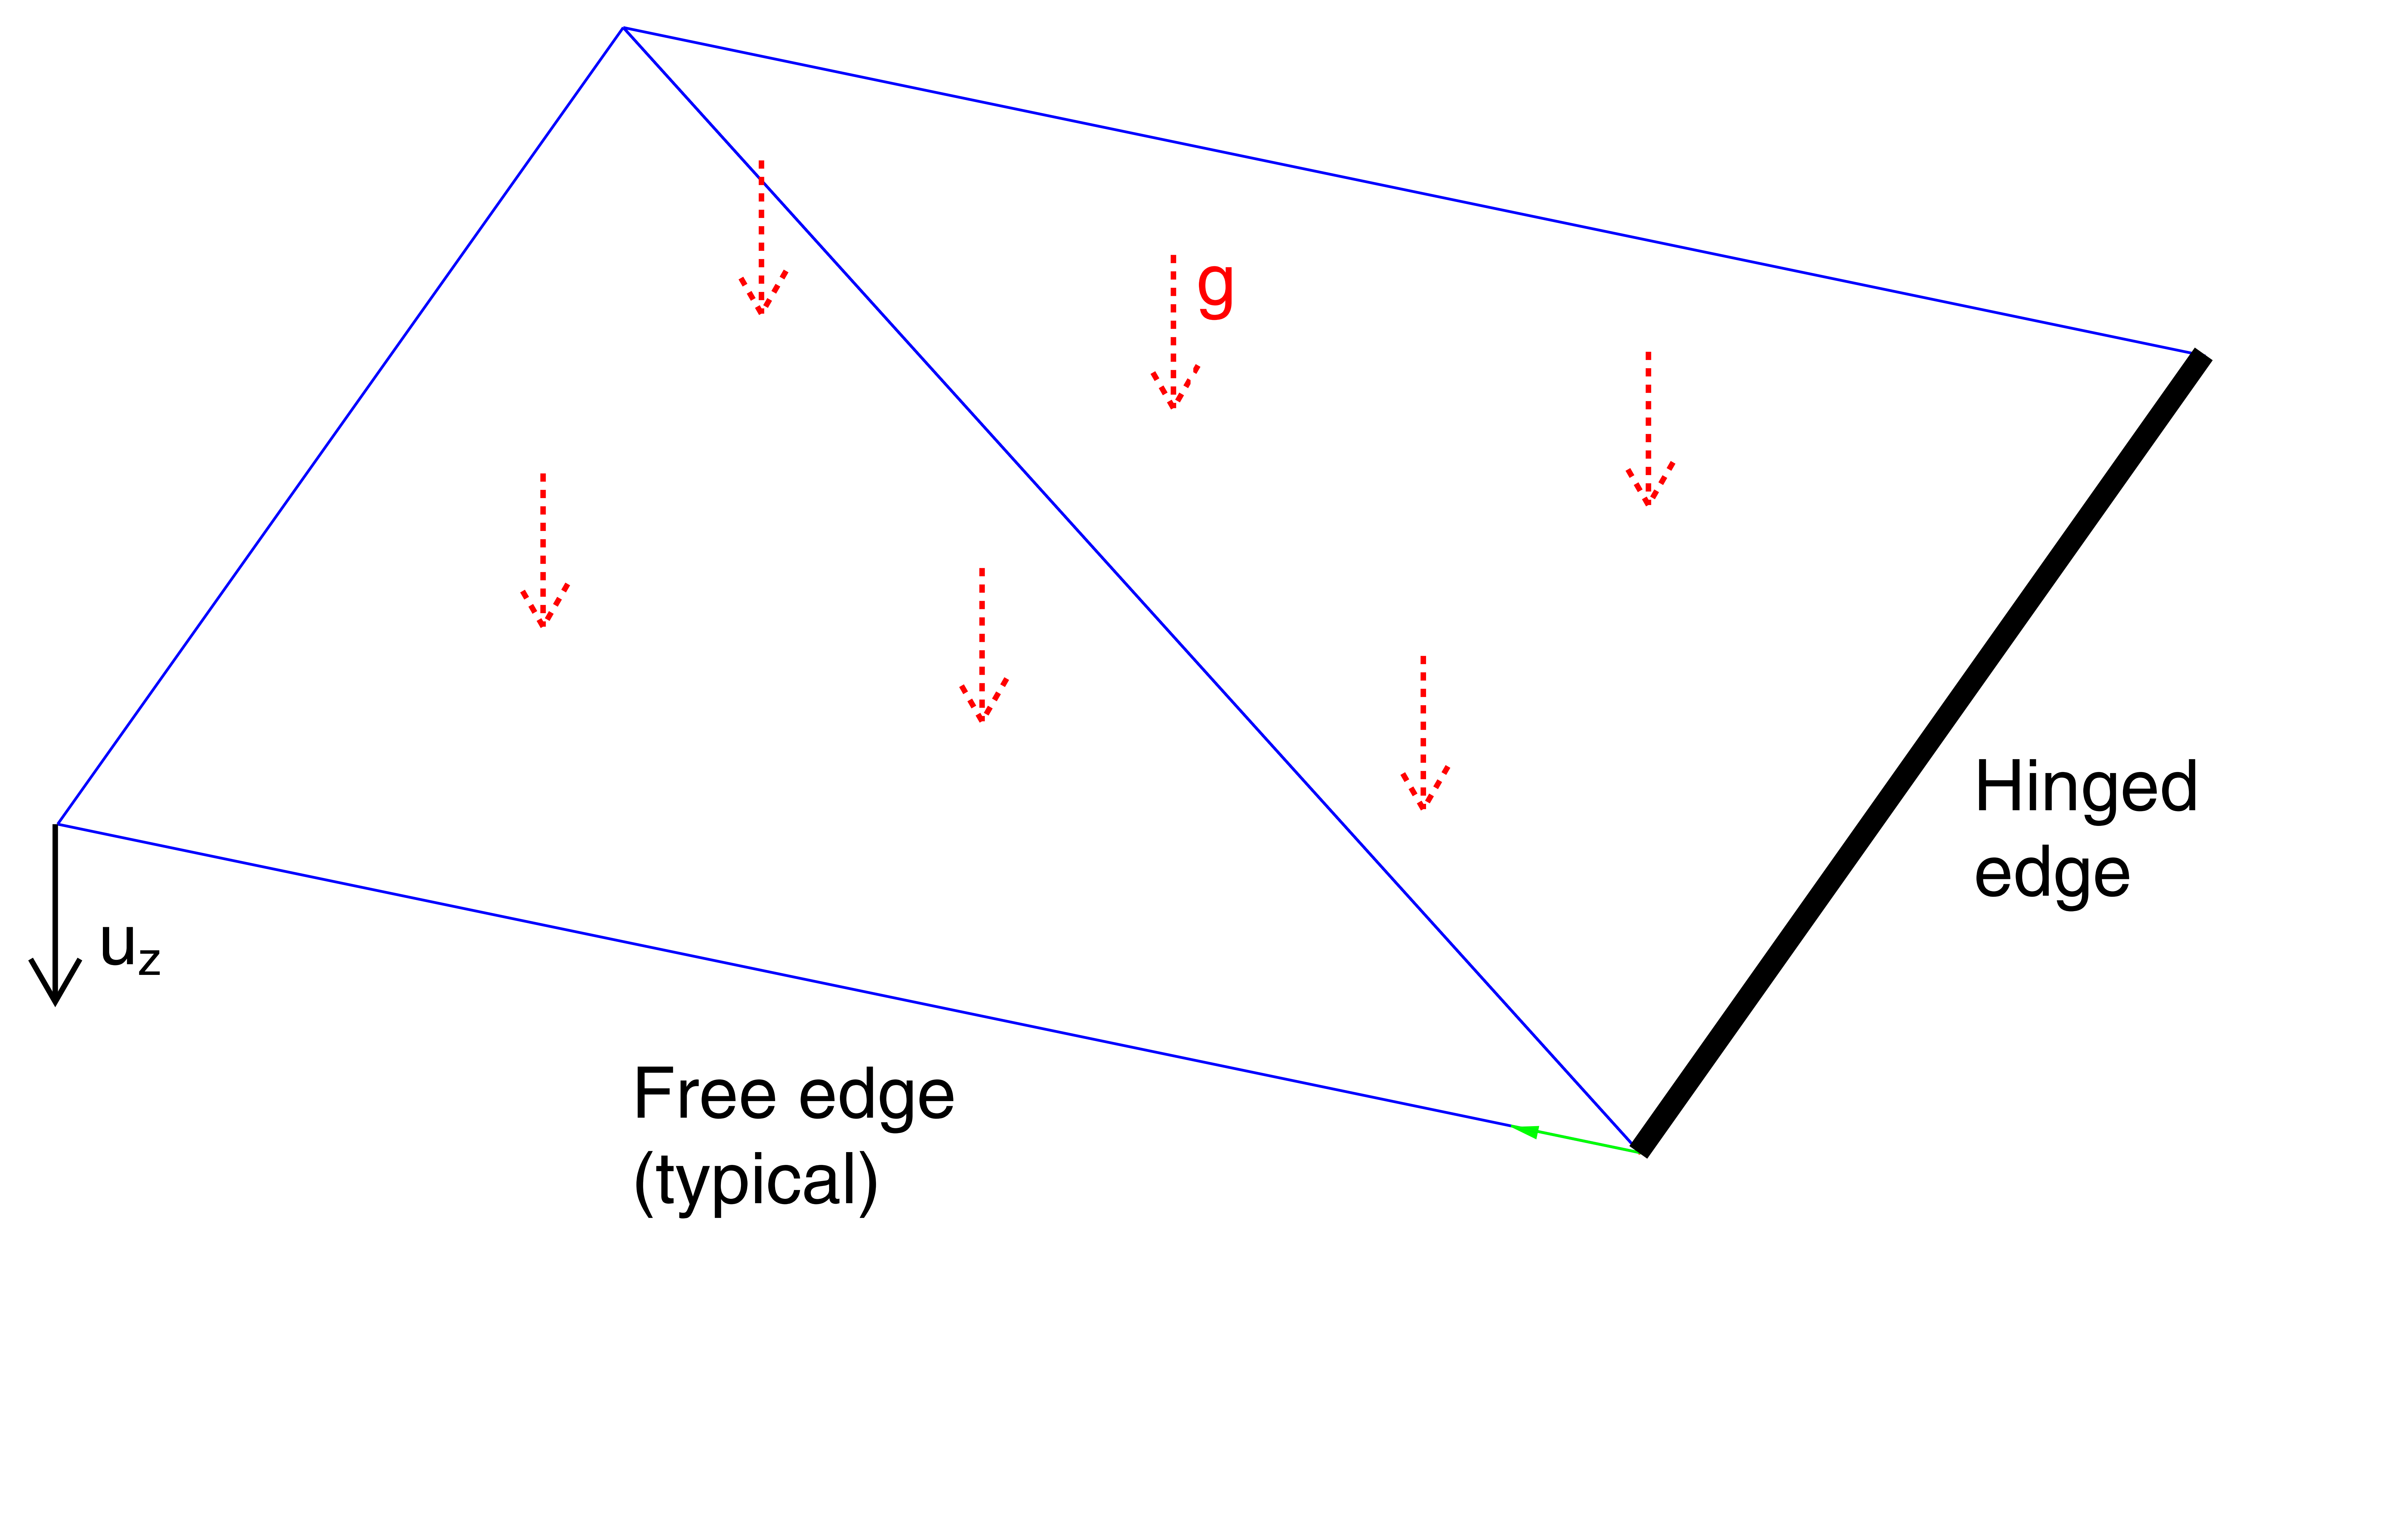
\includegraphics[width=7.3cm]{images/swinging_plate_problem.png}
	\caption{Shell pendulum definition}
\end{figure}
\begin{figure}[H]
	%\centering
	\subfloat[Results using lumped mass matrices]
	{\label{ref_label1}
		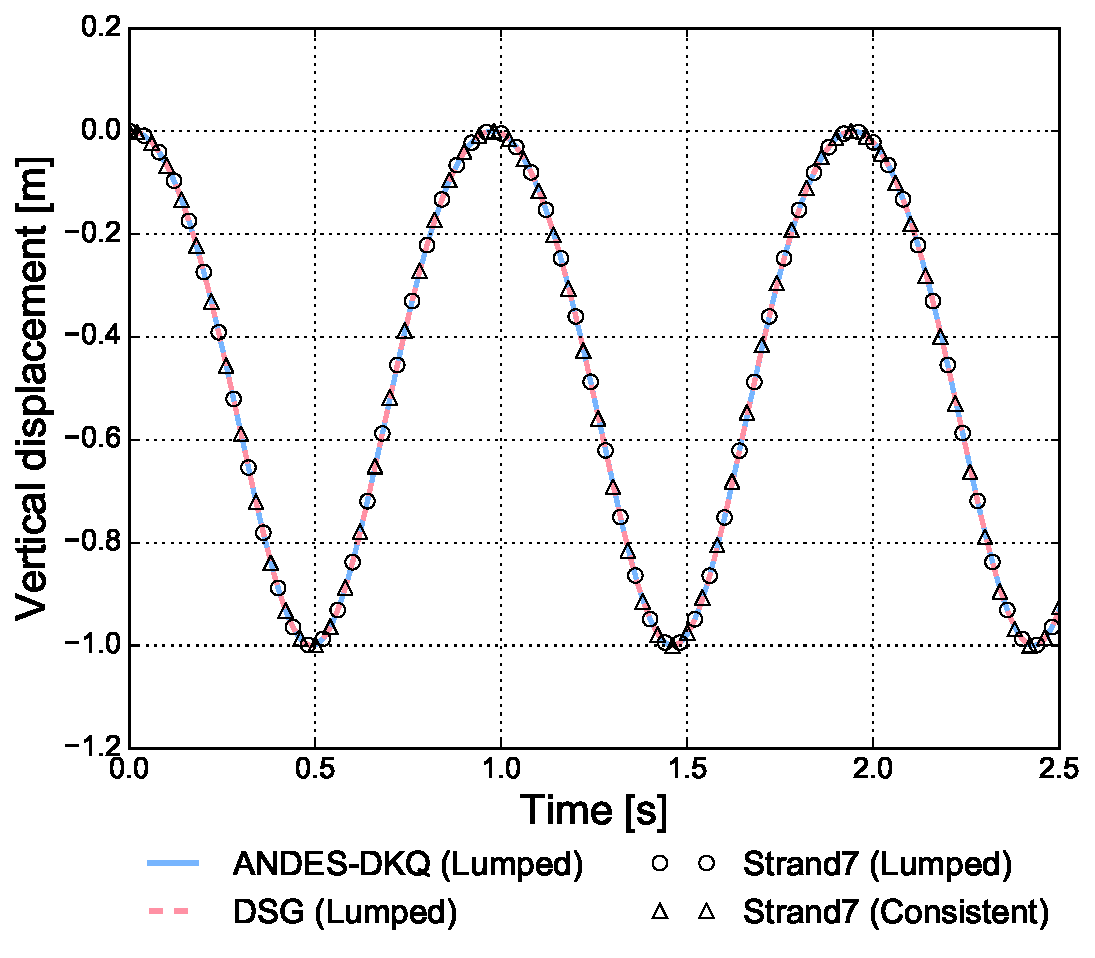
\includegraphics[width=7.3cm]
		{images/shell_pendulum_lumped.pdf}}
	\subfloat[Results using consistent mass matrices]
	{\label{ref_label2}
		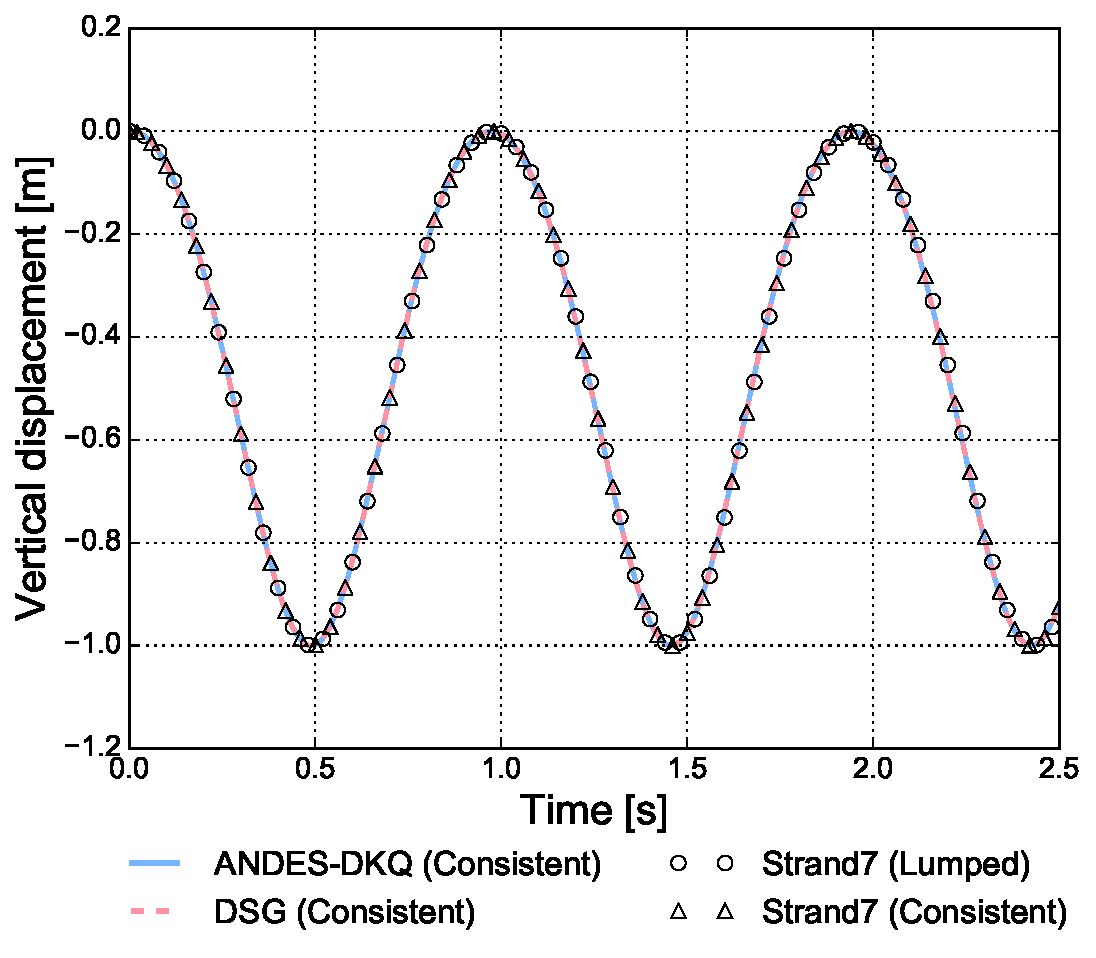
\includegraphics[width=7.3cm]
		{images/shell_pendulum_consistent.pdf}}
	\caption{\label{ref_label_overall}Vertical displacement over time of the shell pendulum analysis}
\end{figure}

The plot of displacement over time demonstrates the ability of both elements to handle large displacements and rotations, agreeing with the reference solution of the existing Kratos quadrilateral shell element. As expected, the minimum vertical displacement of $u_z=-1m$ corresponds to the position of bottom dead centre of the plate, while the maximum vertical displacement of $u_z=0m$ corresponds to a fully horizontal plate orientation

\subsection{Oscillating clamped plate}

The oscillating clamped plate benchmark subjects a clamped cantilever square plate $2m\times2m\times0.1m$ thick to a uniform globally oriented surface pressure of $P_z = -0.25 Pa$. The plate material is linear elastic characterised by $E = 1\times 10^6 Pa,\ \nu = 0.0$ and $\rho = 7850 kg/m^3$. The key result is the vertical displacement component of the free corner node as illustrated below.

\begin{figure}[H]
	\centering
	\def\svgwidth{\columnwidth}
	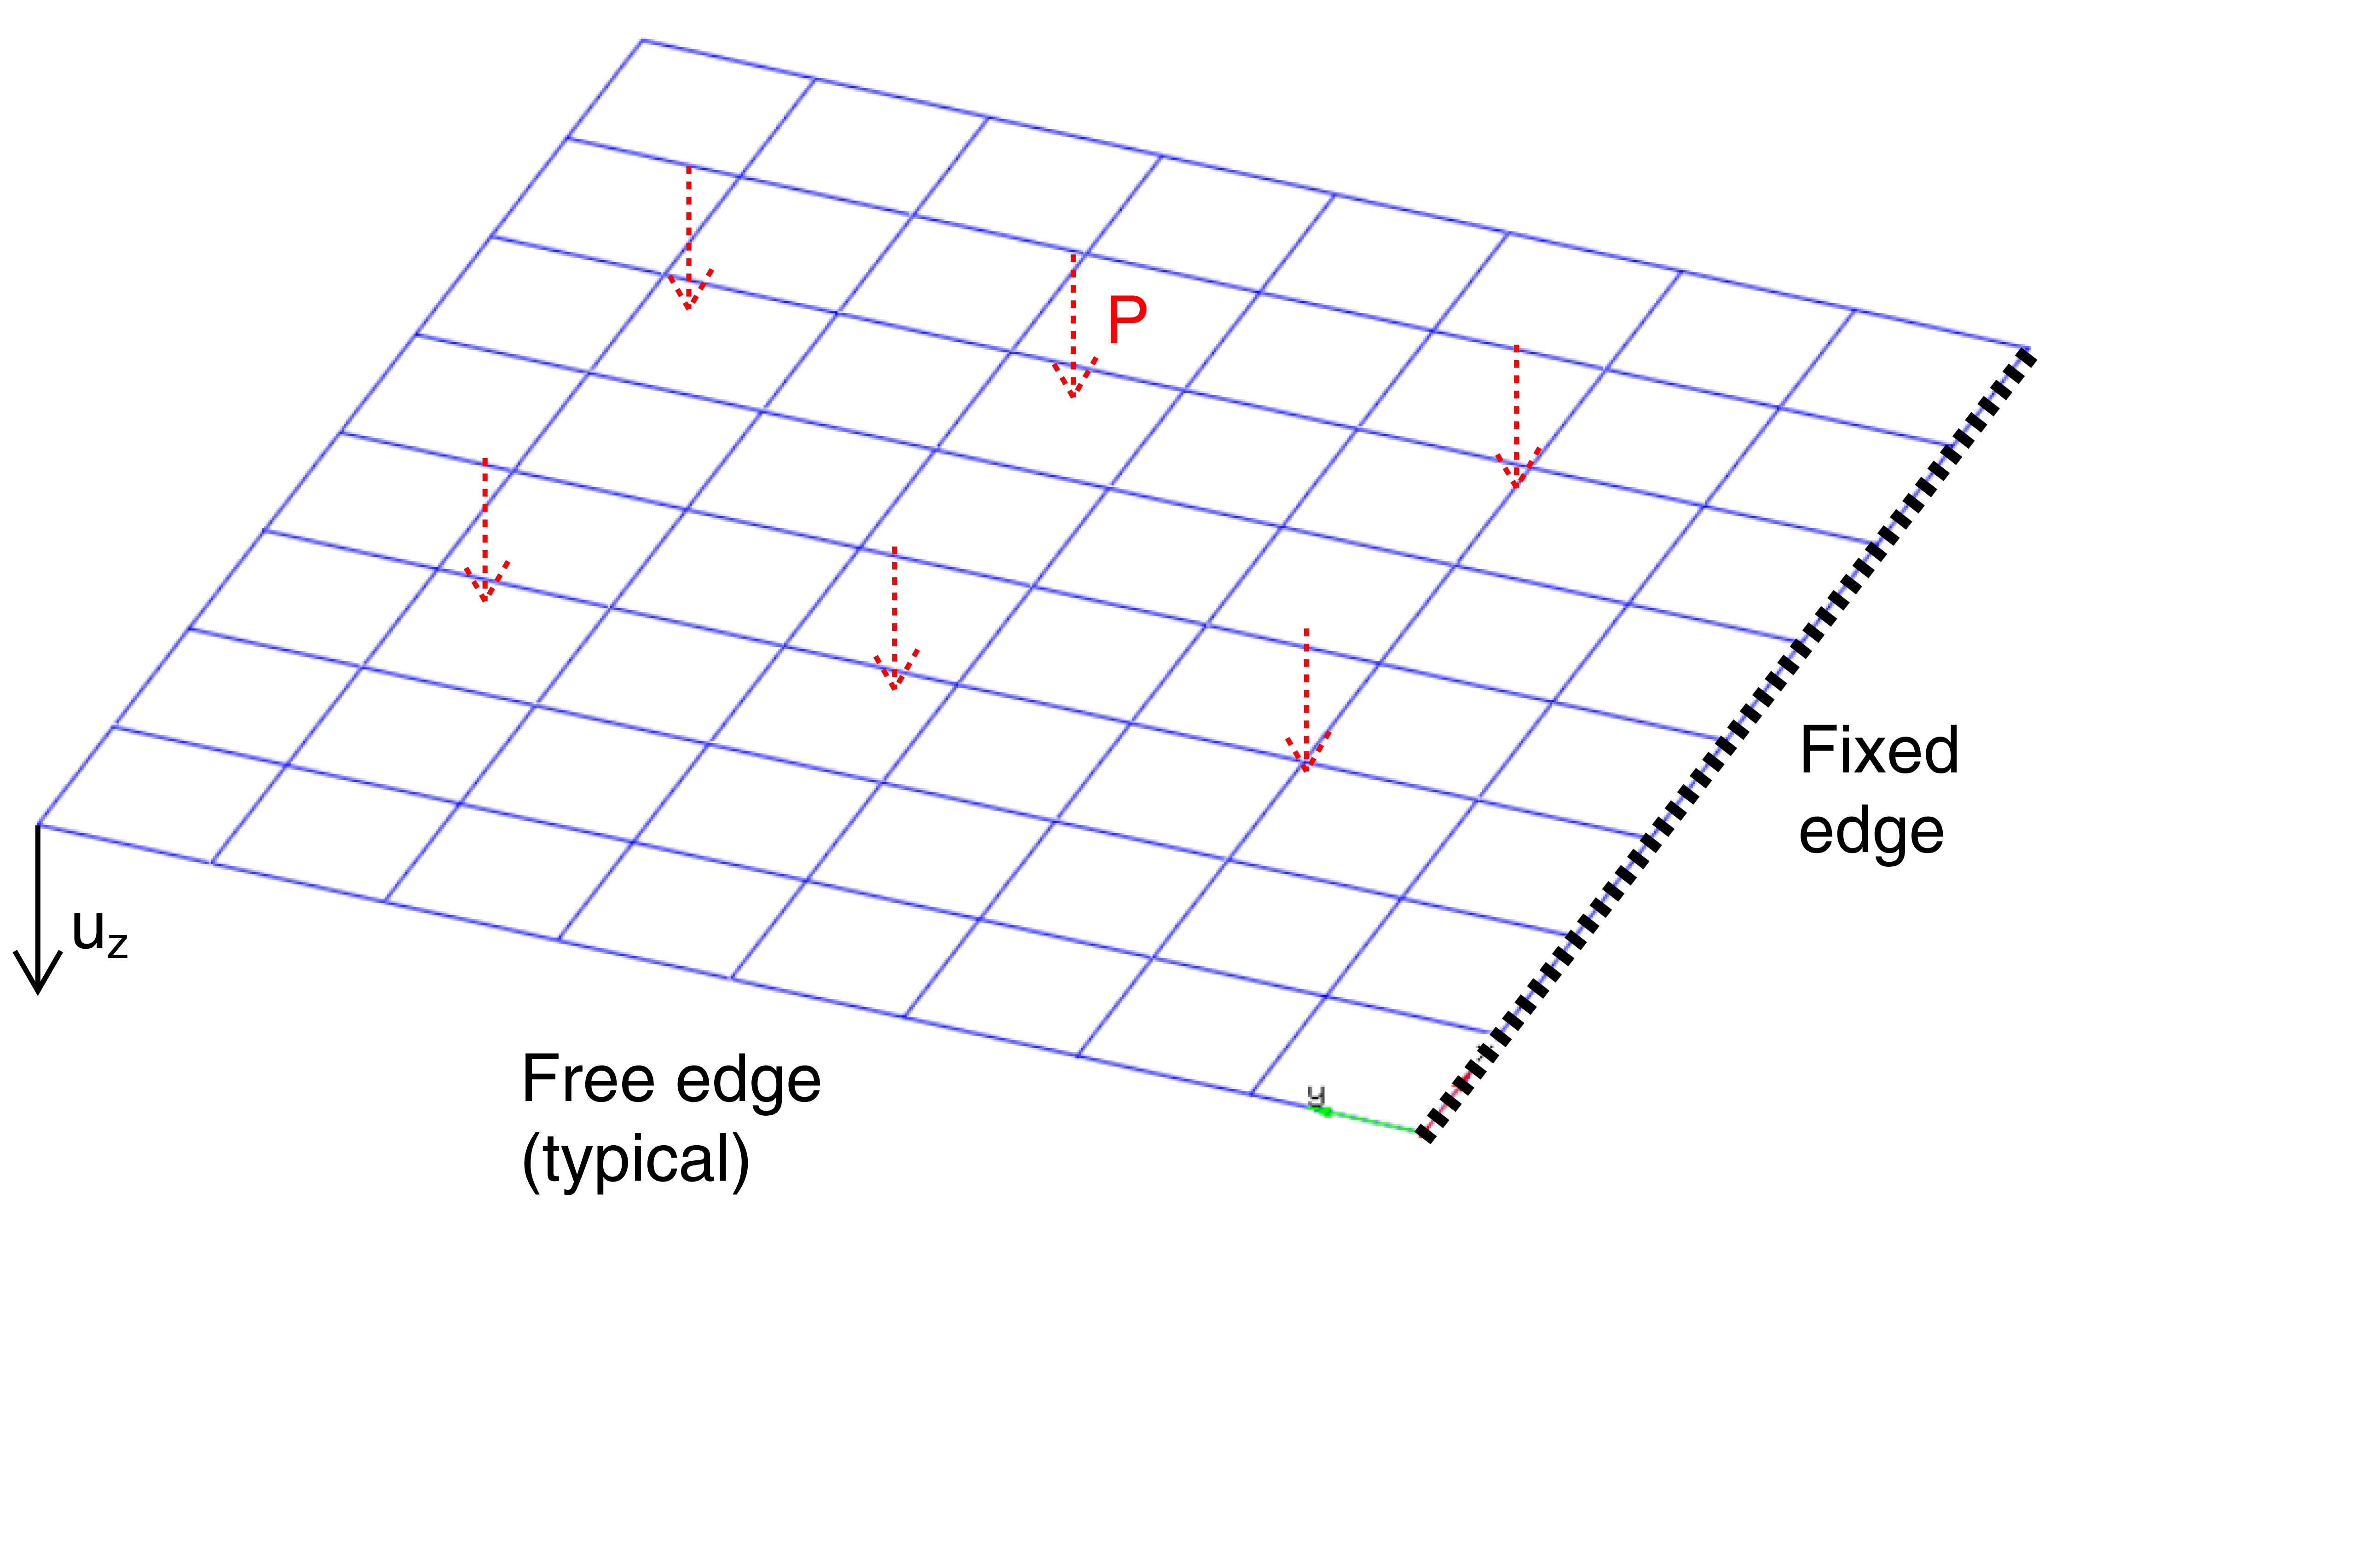
\includegraphics[width=7.3cm]{images/quad_bend_problem.png}
	\caption{Oscillating clamped plate definition}
\end{figure}
\begin{figure}[H]
	%\centering
	\subfloat[Results using lumped mass matrices]
	{\label{ref_label1}
		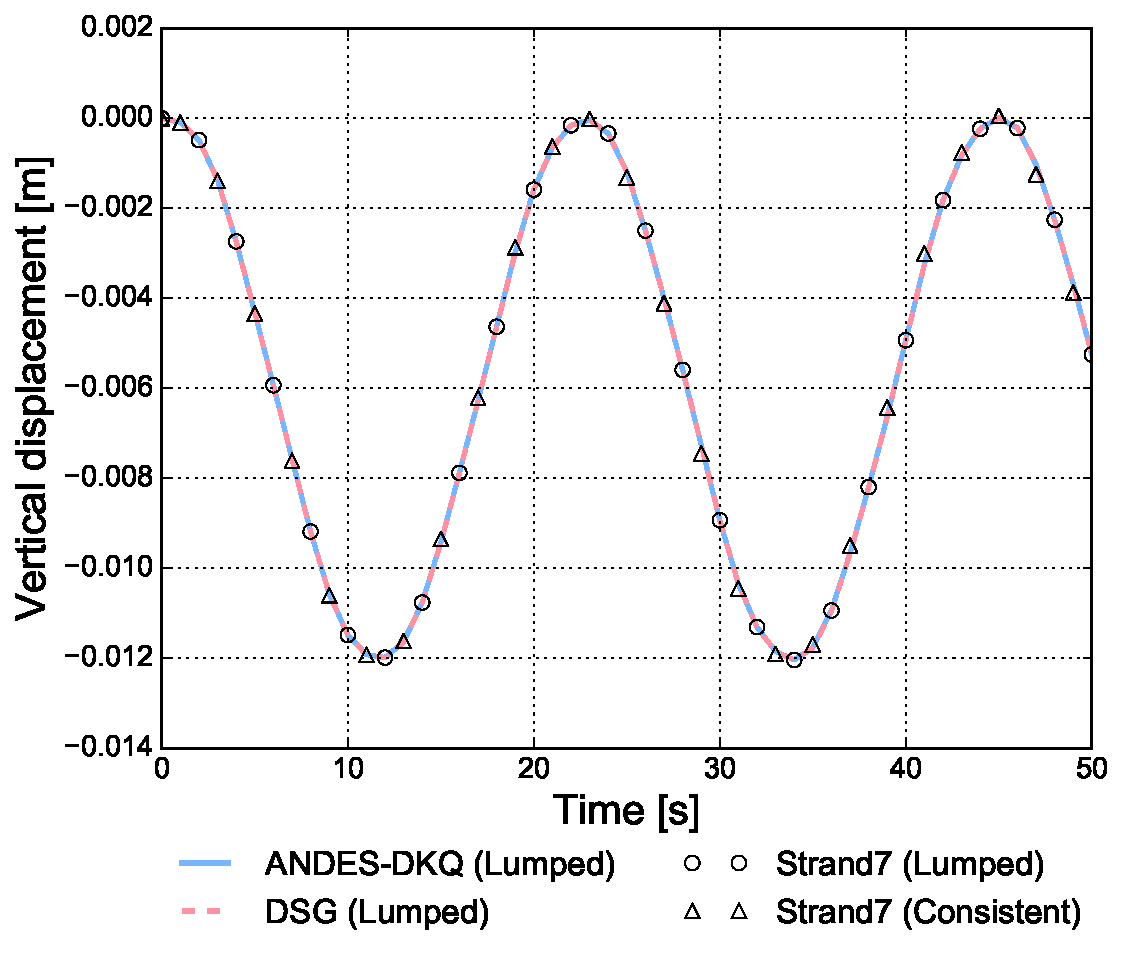
\includegraphics[width=7.3cm]
		{images/oscillating_plate_lumped.pdf}}
	\subfloat[Results using consistent mass matrices]
	{\label{ref_label2}
		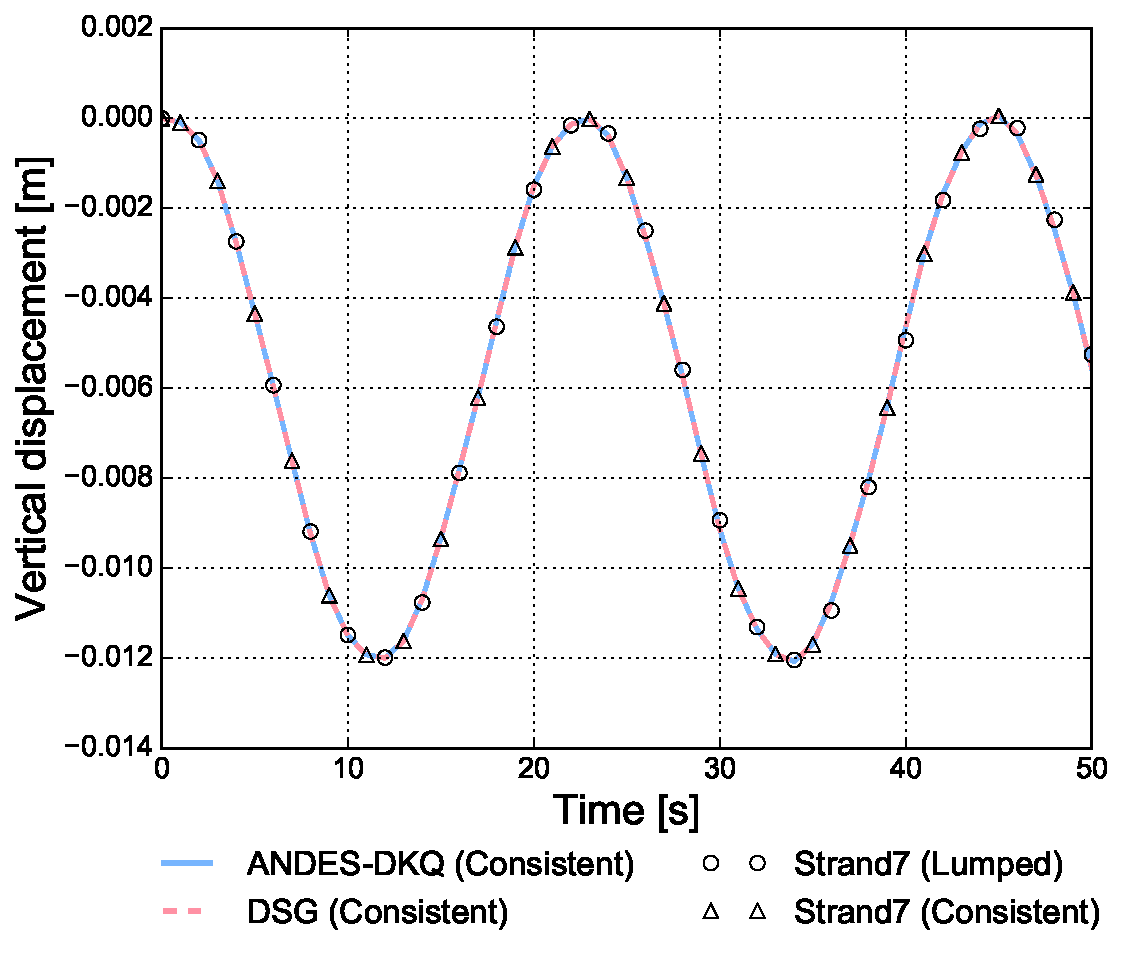
\includegraphics[width=7.3cm]
		{images/oscillating_plate_consistent.pdf}}
	\caption{\label{ref_label_overall}Vertical displacement over time of the oscillating clamped plate analysis}
\end{figure}

 The plot of vertical displacement over time demonstrates both elements agree with the reference solution, which is the existing Kratos quadrilateral element. The overall results correctly correspond to structural dynamics theory by oscillating with the base natural frequency about the static displacement of $u_z=-0.006m$.

\section{Quantity recovery tests}

Although displacements are the primary solution variables of a finite element analysis, recovered quantities, such as strains, stresses and force resultants are often more determinant to the success or failure of a system. The following tests validate the implemented elements ability to correctly recovery these quantities.

\subsection{Simply supported dome with oculus under self weight}
\label{subsection:dome_test}

A simply supported dome with an oculus under self weight is considered to evaluate the membrane results of the elements. The hemi-spherical dome is defined by the following parameters: $R = 5m,\ h = 0.01m,\ \rho = 7850 kg/m^3,\ g = 9.81m/s^2,\ E = 2 \times 10^{11} Pa,\ \nu = 0.3$. The 20 degree opening has no edge loading. Appendix \ref{app:Analytical membrane analysis of dome} derives the analytical formulae which form the reference solution for both force resultants, while an analysis of the problem with ANSYS provides the Von Mises stress reference solution.

\begin{figure}[H]
	%\centering
	\subfloat[Circumferential shell force over meridian angle]
	{\label{ref_label1}
		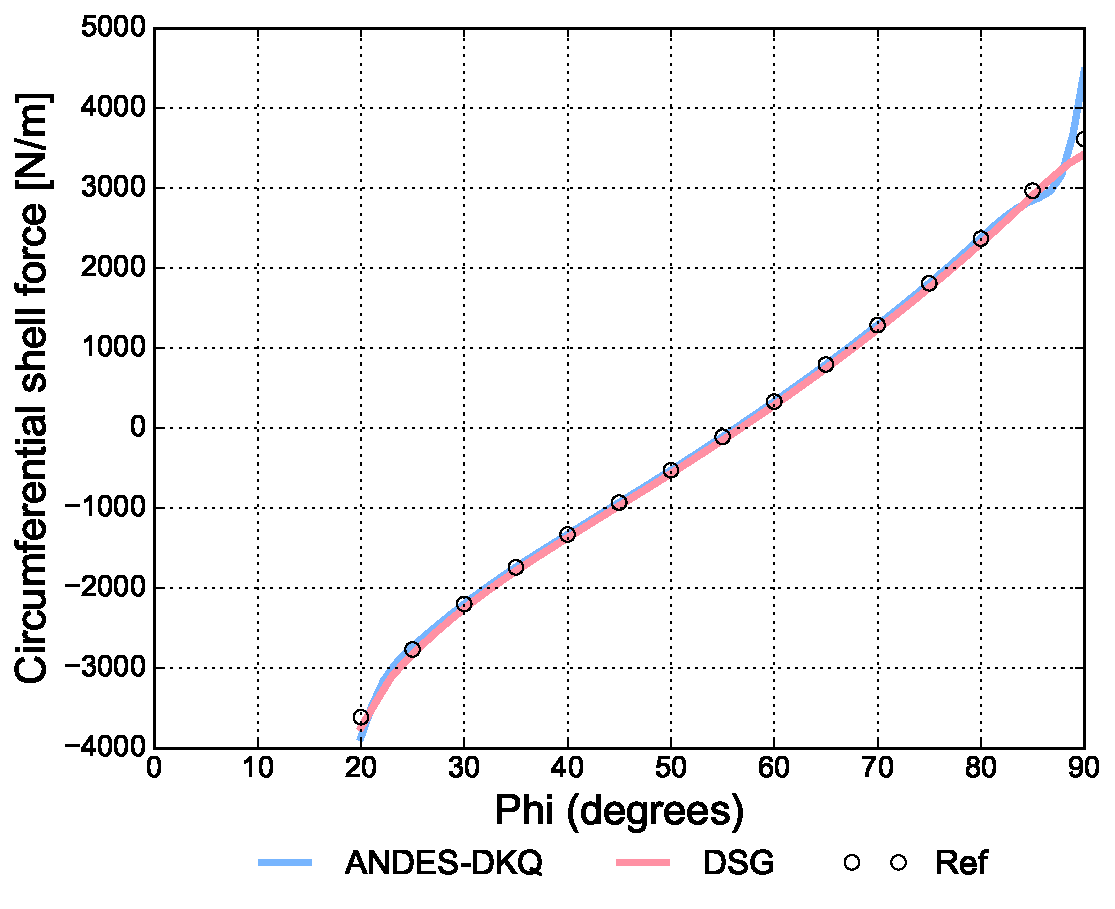
\includegraphics[width=7.3cm]
		{images/Simply_support_dome_n_theta.pdf}}
	\subfloat[Meridional shell force over meridian angle]
	{\label{ref_label2}
		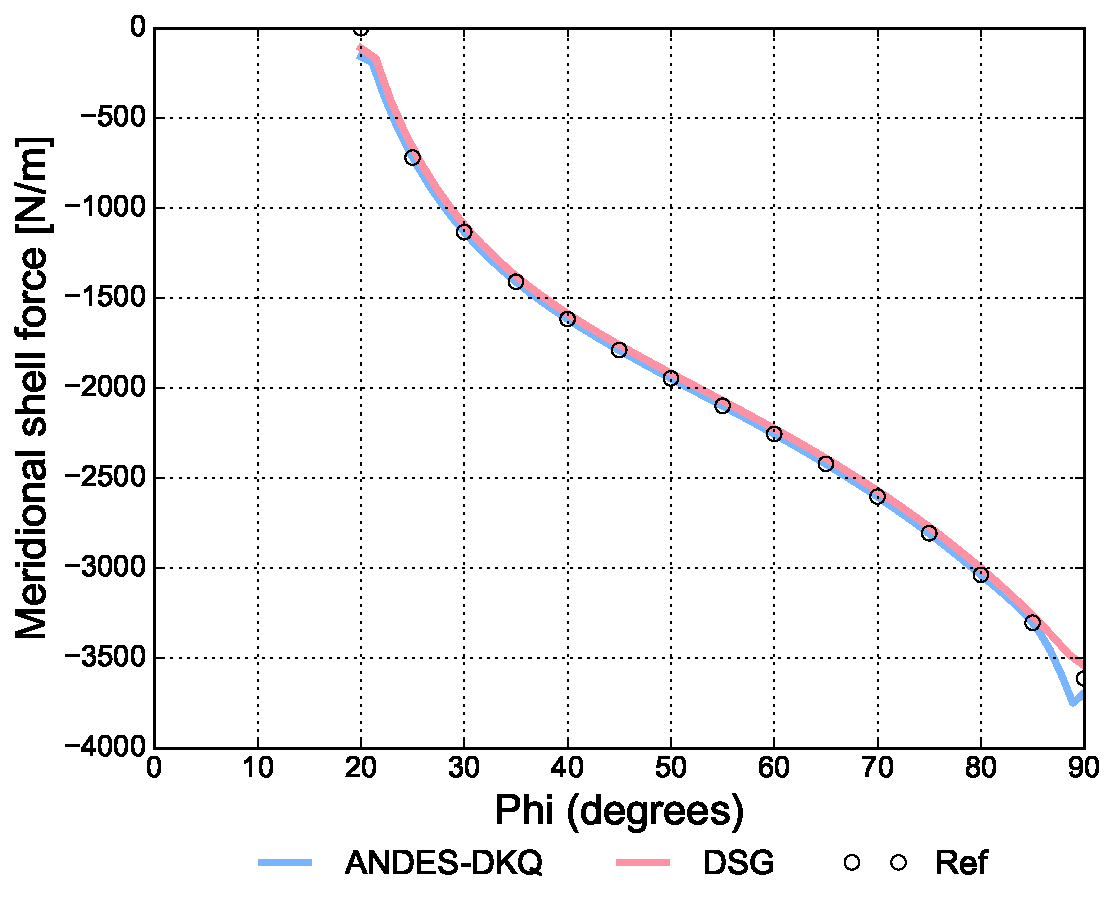
\includegraphics[width=7.3cm]
		{images/Simply_support_dome_n_phi.pdf}}
	\\
		\subfloat[Mid-plane Von Mises stress over meridian angle]
	{\label{ref_label1}
		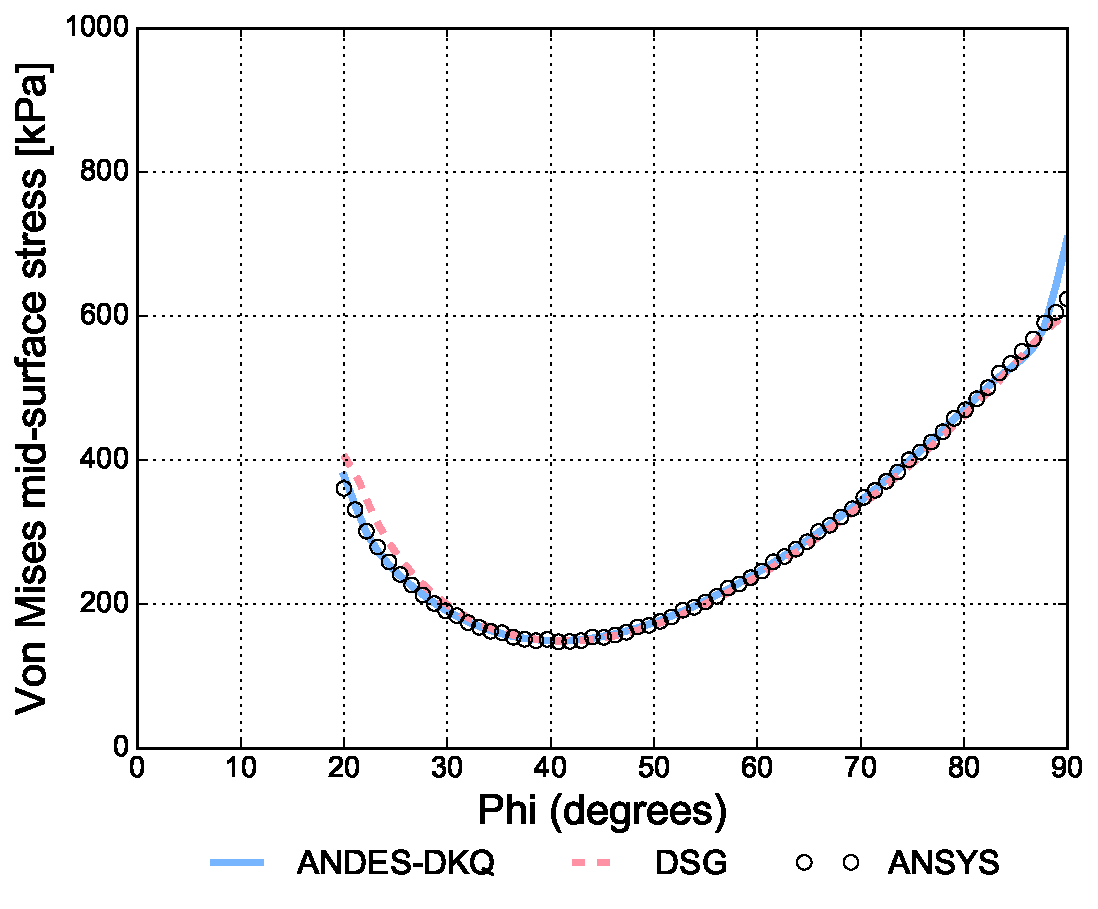
\includegraphics[width=7.3cm]
		{images/Simply_support_dome_von_mises.pdf}}
	\subfloat[Mid-plane Von Mises plot of the reference ANSYS solution]
	{\label{ref_label2}
		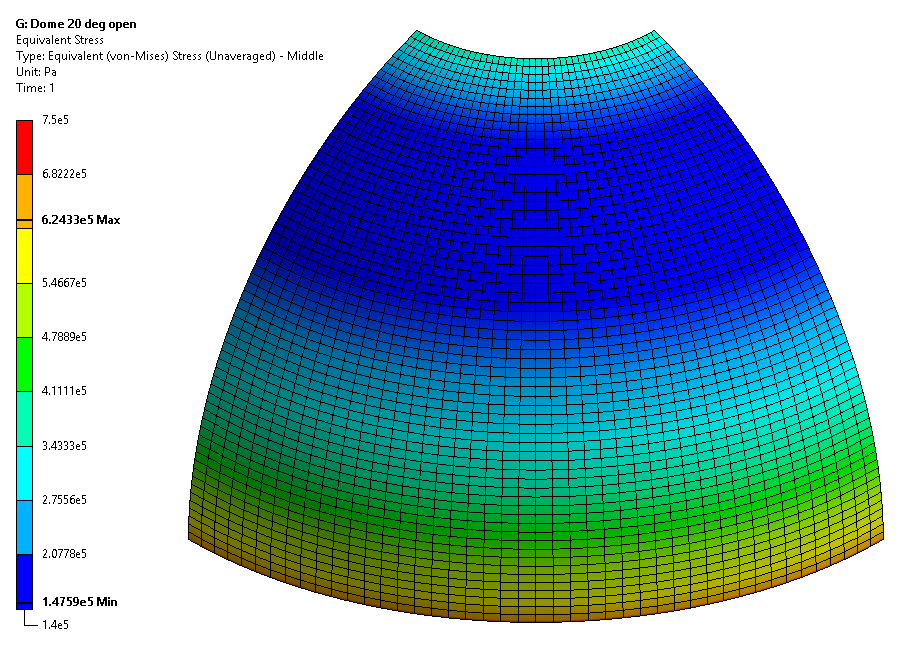
\includegraphics[width=7.3cm]
		{images/simply_support_dome_ansys_vm_plot.png}}
	\\
	\subfloat[Mid-plane Von Mises plot of the ANDES solution]
	{\label{ref_label1}
		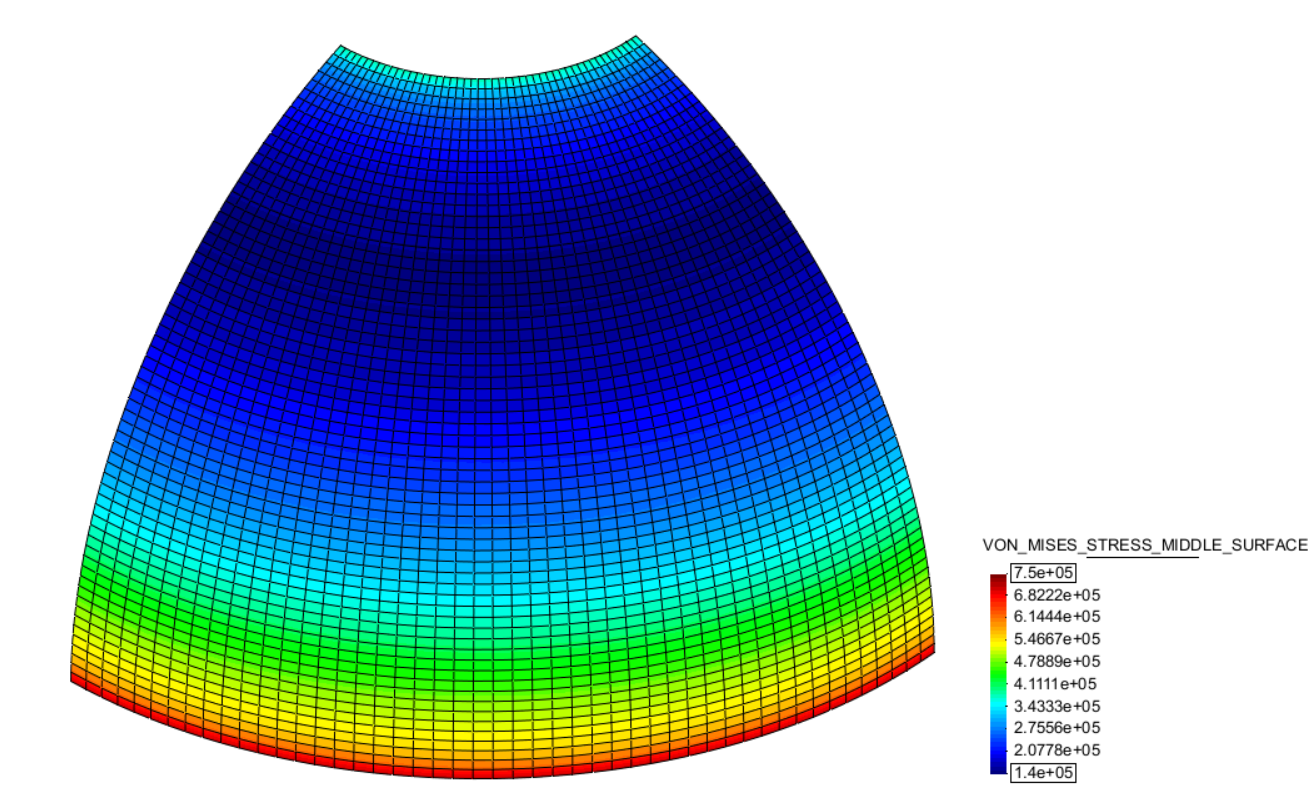
\includegraphics[width=7.3cm]
		{images/simply_support_dome_andes_vm_plot.png}}
	\subfloat[Mid-plane Von Mises plot of the DSG solution]
	{\label{ref_label2}
		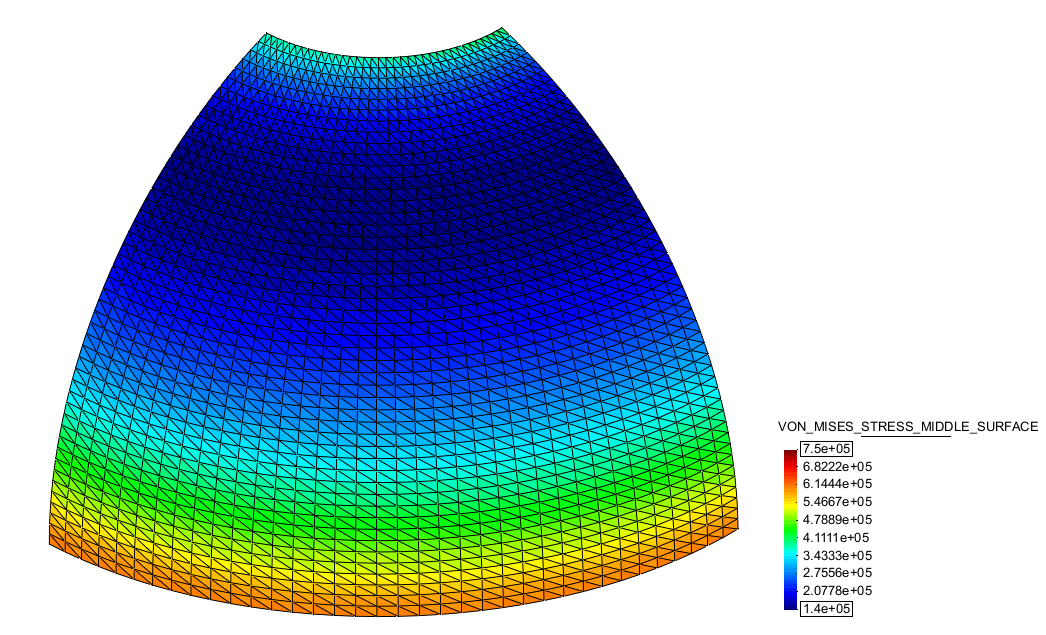
\includegraphics[width=7.3cm]
		{images/simply_support_dome_dsg_vm_plot.png}}
	\caption{\label{Shell_force_dome_benchmark_shell_force}Results of the simply supported dome analysis}
\end{figure}

The results of both elements for circumferential and meridional shell forces demonstrate excellent agreement with the analytical membrane analysis. Minor deviations occur at both ends of the dome due to the strict assumptions of the analytical membrane theory and mesh effects. The mid-surface Von Mises stress results also agree with the ANSYS solution quite closely, with the ANDES-DKQ slightly out-performing the DSG element. The contour plots (with all limits set to $[1.4\times 10^5,\ 7.5\times10^5]$) further exhibit the similarities between the three solution methods.
%limits all set to [1.4e5, 7.5e5] !!!!!!
\subsection{Navier supported plate under sinusoidal load}
\label{validation:navier plate under sinusoidal load}
A Navier supported square plate subject to a sinusoidal load is considered to examine the bending stress results of the ANDES-DKQ element. A 3-parameter analytical solution forms the reference for this problem \cite{reddy2004mechanics}. 

\begin{figure}[H]
	\centering
	\def\svgwidth{\columnwidth}
	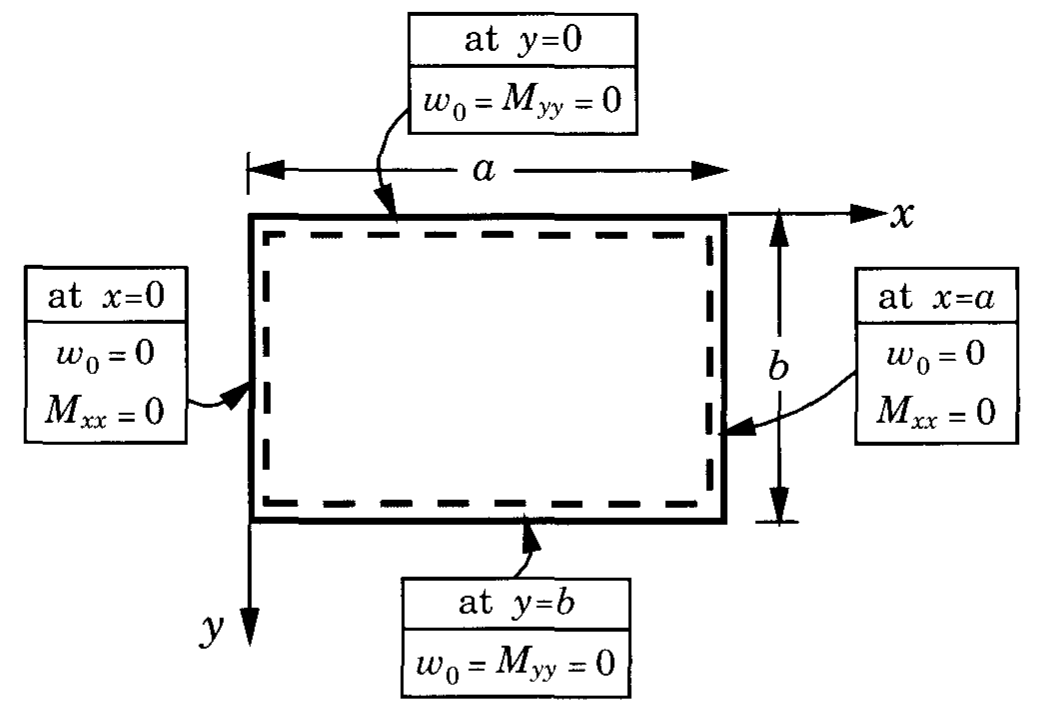
\includegraphics[width=7.3cm]{images/navier_plate_def.png}
	\caption{Definition of the Navier supported plate test \cite{reddy2004mechanics}}
	\label{validation:pic navier plate}
\end{figure}

Due to symmetry, one quarter of a $a = 200,\ b = 200,\ h = 10$ square plate of linear isotropic material $E = 2\times 10^{11}$ and $\nu = 0.3$ is modelled and subject to a spatially varying transverse pressure of $q = -1\times 10^7 sin(\frac{x\pi}{200})sin(\frac{y\pi}{200})$. The following graphs plot quantities along a path from $x=0$ to $x=100$ at $y=100$.

\begin{figure}[H]
	%\centering
	\subfloat[Normal stress (XX) over X coordinate]
	{\label{ref_label1}
		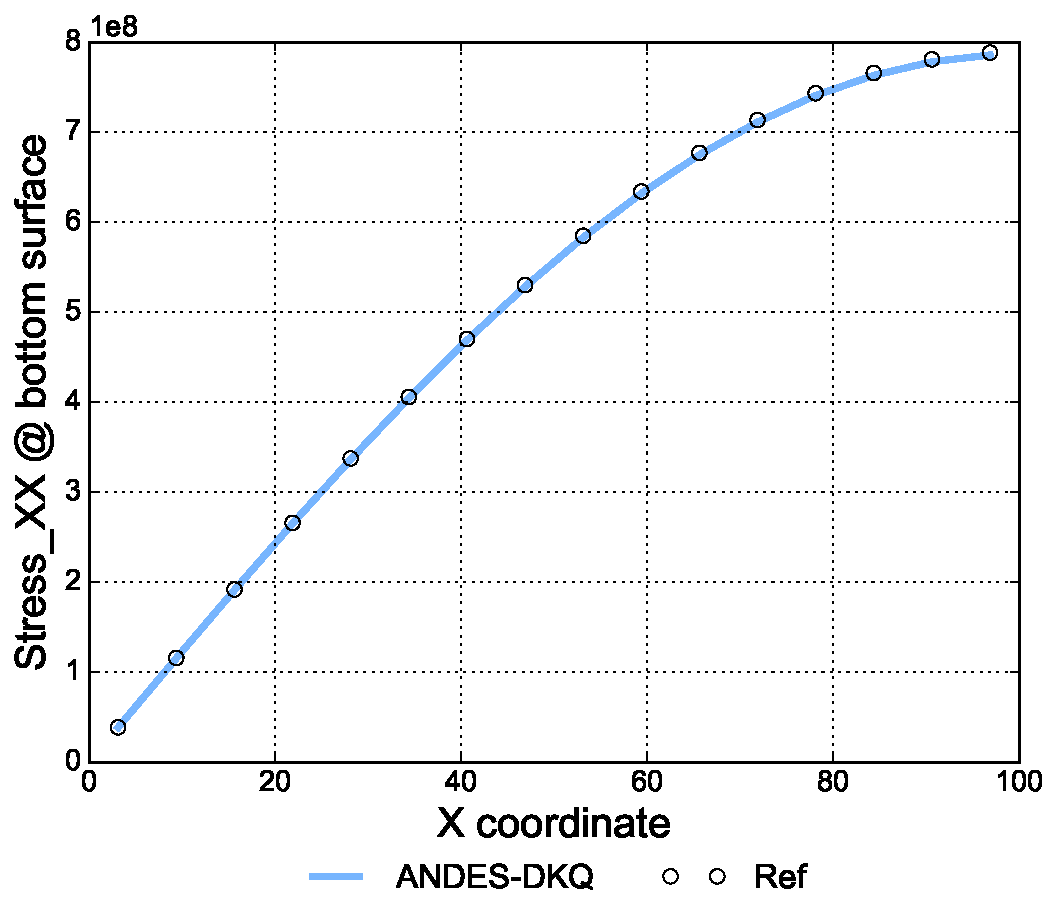
\includegraphics[width=7.3cm]
		{images/navier_plate_quad_s_xx_bot.pdf}}
	\subfloat[Normal stress (YY) over X coordinate]
	{\label{ref_label2}
		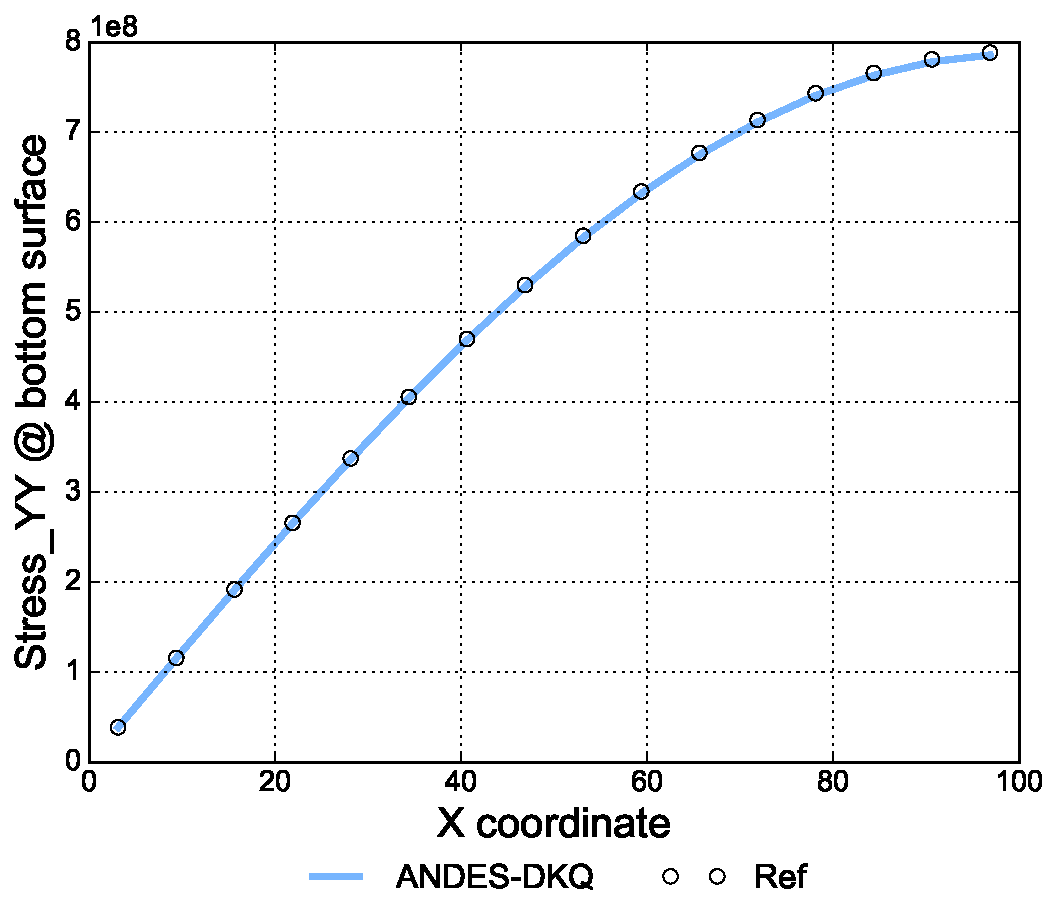
\includegraphics[width=7.3cm]
		{images/navier_plate_quad_s_yy_bot.pdf}}
	\\
	\subfloat[Shear stress (XY) over X coordinate]
	{\label{ref_label1}
		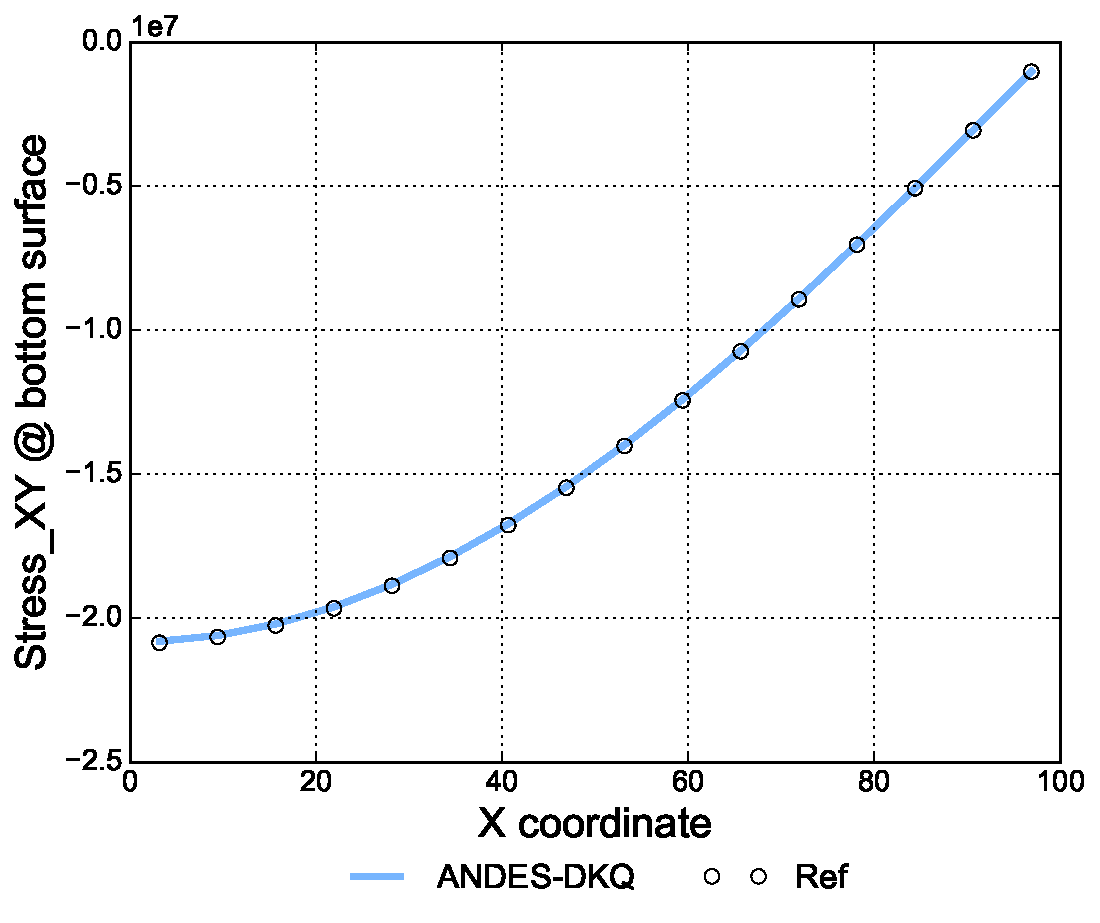
\includegraphics[width=7.3cm]
		{images/navier_plate_quad_s_xy_bot.pdf}}
	\subfloat[Von Mises stress over X coordinate]
	{\label{ref_label2}
		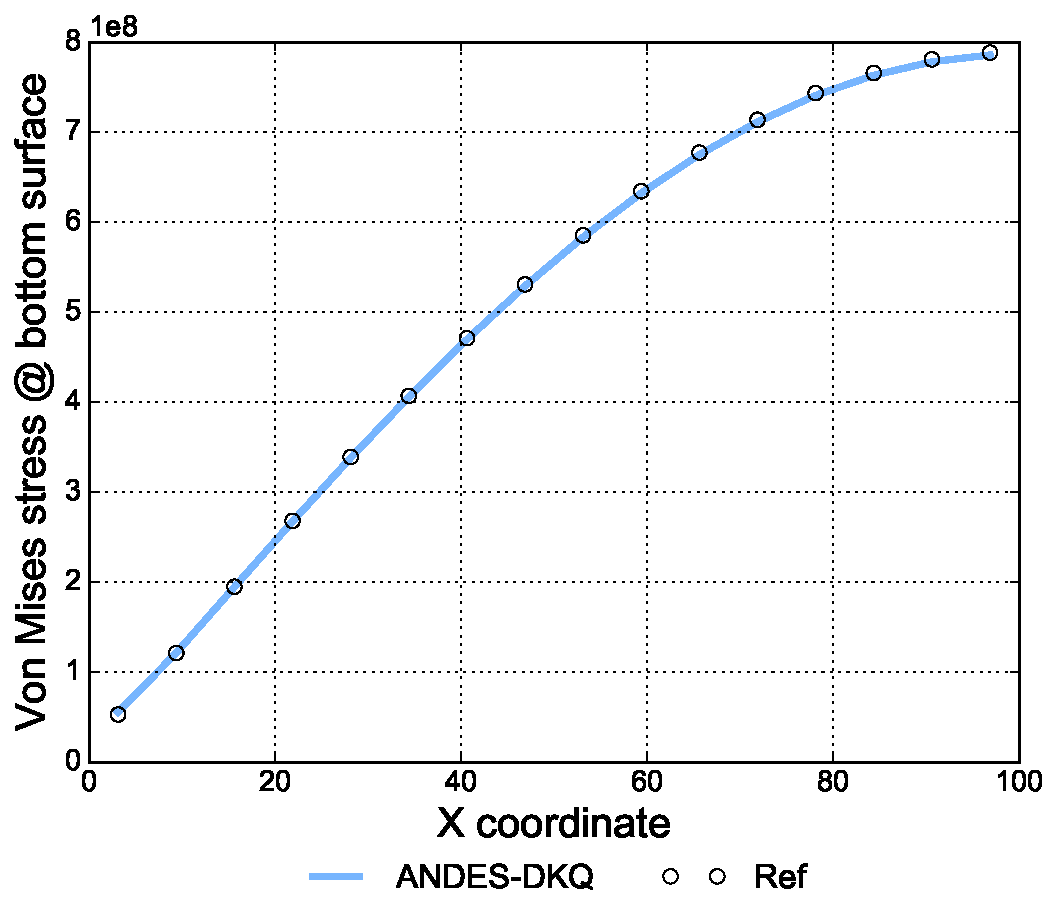
\includegraphics[width=7.3cm]
		{images/navier_plate_quad_s_vm_bot.pdf}}
	\caption{\label{Navier_quad_s_xx_yy}Stresses (bottom surface) of the Navier supported plate under sinusoidal load}
\end{figure}

The above figures demonstrate exemplary alignment between the analytical solution and the ANDES-DKQ element across all stresses considered.

\subsection{Navier supported plate under uniformly distributed load}
\label{validation:DSG navier unifom}

A Navier supported square plate subject to a uniformly distributed load is considered to examine the bending stress results of the DSG element. An ANSYS analysis forms the reference for this problem. The problem setup is identical to the preceding test with the exception of a uniformly distributed transverse pressure $q = -1\times 10^{11}$ and "hard" supports along the edges ($\phi_x = 0$ on edges parallel to y-axis, $\phi_y = 0$ on edges parallel to x-axis).

Graphs plotted along an X coordinate follow the same path as the preceding tests. Graphs plotted along a Y coordinate run from $y = 0$ to $y = 100$ with $x = 100$, while graphs plotted along a diagonal distance run from $x=y=0$ to $x=y=100$.
%
%\begin{figure}[h!]
%	\centering
%	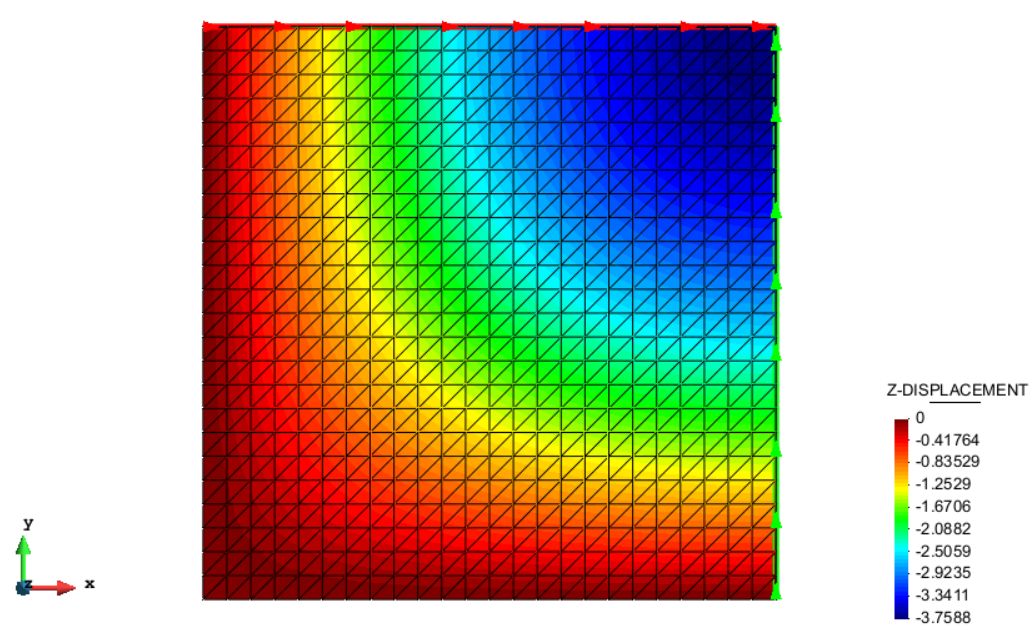
\includegraphics[width=14cm]{images/navier_thick_tri_paths}
%	\caption{Paths for results: Red = X path and Green = Y path}
%	\label{fig:navierthicktripaths}
%\end{figure}
%
%\newpage

\begin{figure}[h!]
	%\centering
	\subfloat[Normal stress (XX) over X coordinate]
	{\label{ref_label1}
		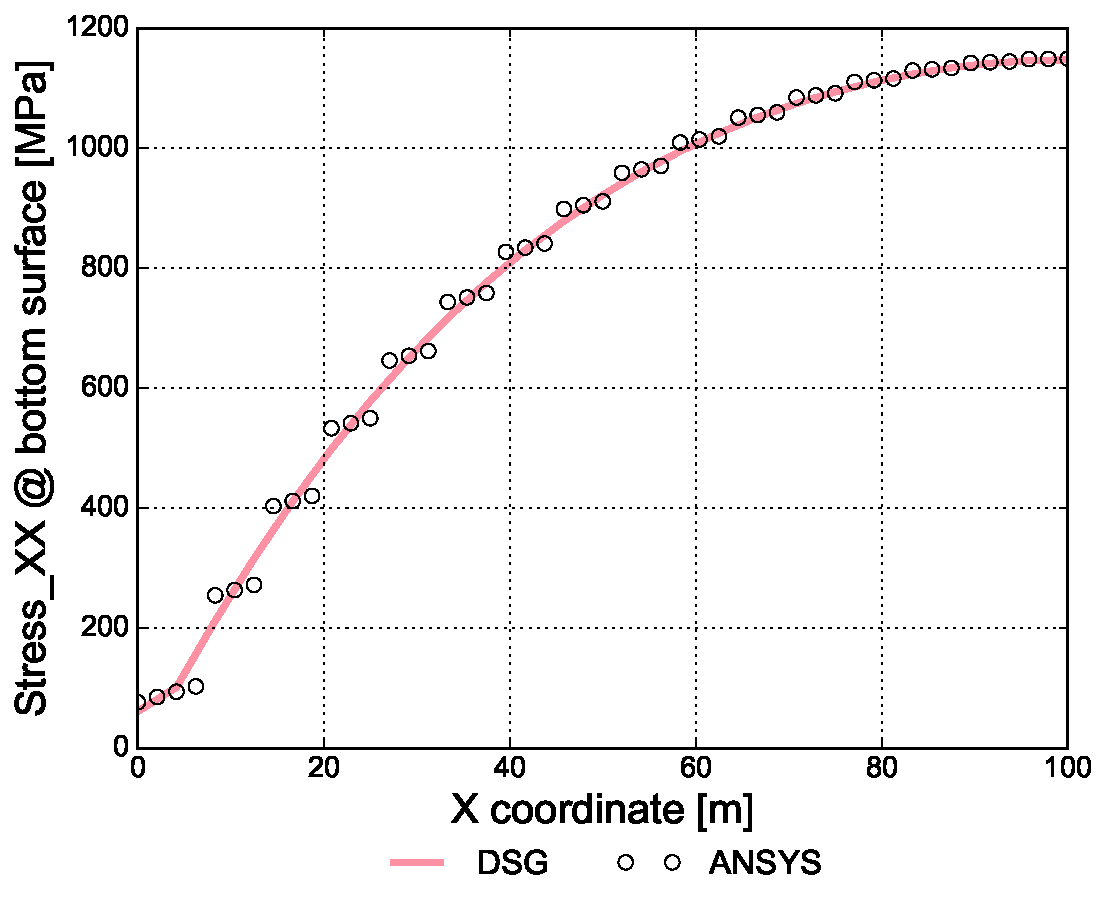
\includegraphics[width=7.3cm]
		{images/navier_plate_tri_s_xx.pdf}}
	\subfloat[Normal stress (YY) over X coordinate]
	{\label{ref_label2}
		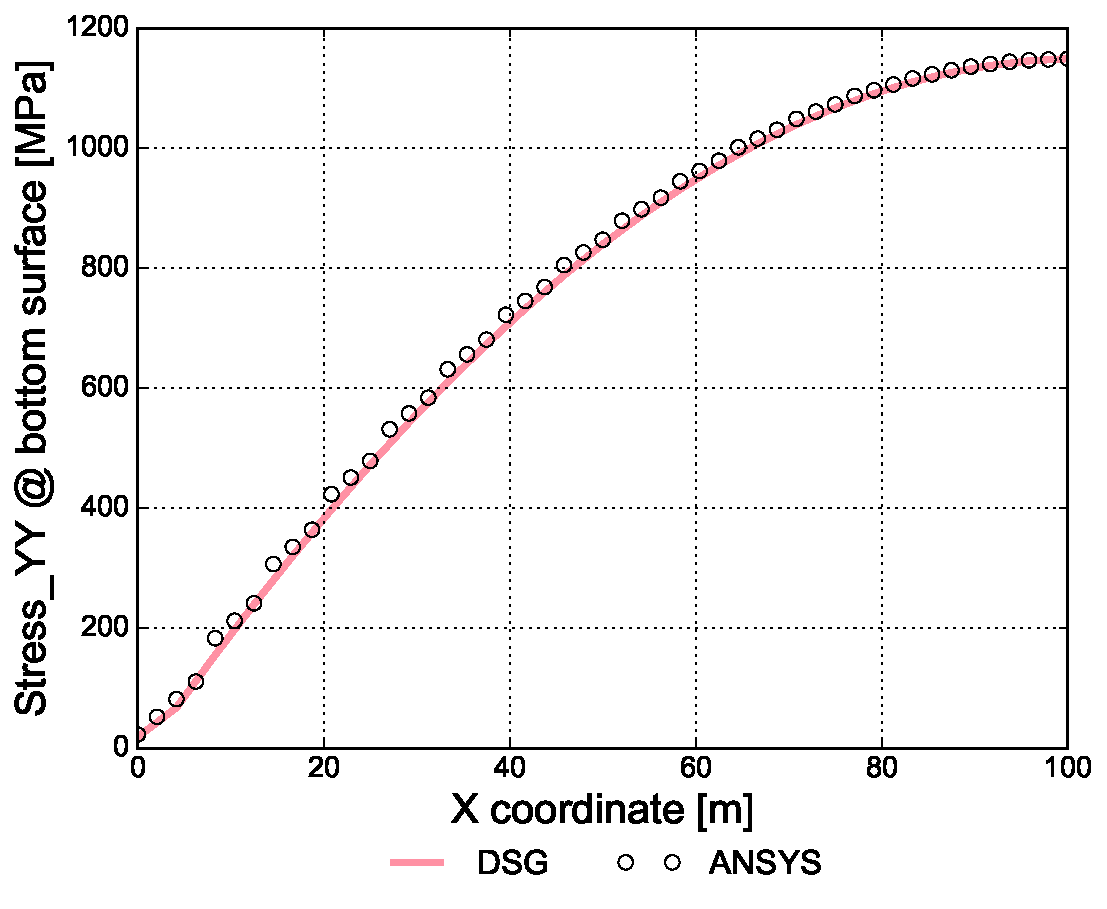
\includegraphics[width=7.3cm]
		{images/navier_plate_tri_s_yy.pdf}}
	\\
	\subfloat[In plane shear stress (XY) over plate diagonal]
	{\label{ref_label1}
		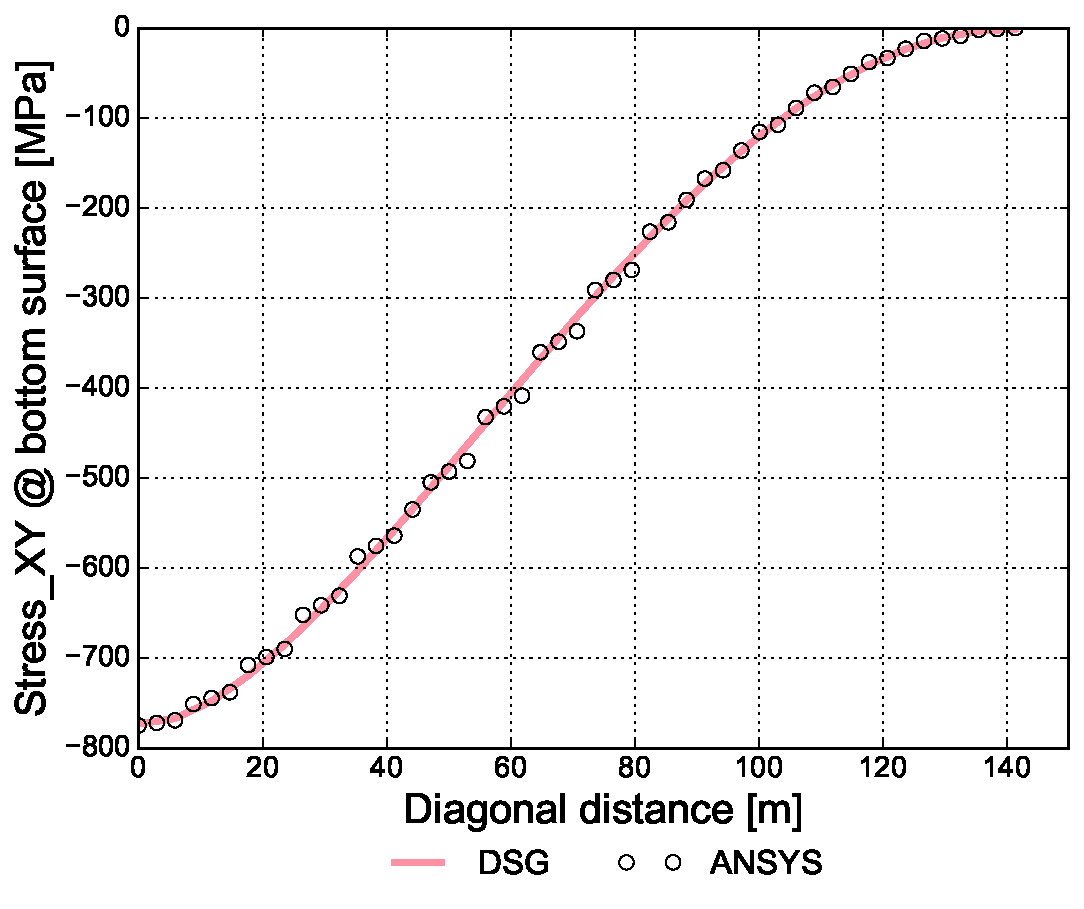
\includegraphics[width=7.3cm]
		{images/navier_plate_tri_s_xy.pdf}}
	\subfloat[Transverse shear stress (XZ) over X coordinate]
	{\label{ref_label1}
		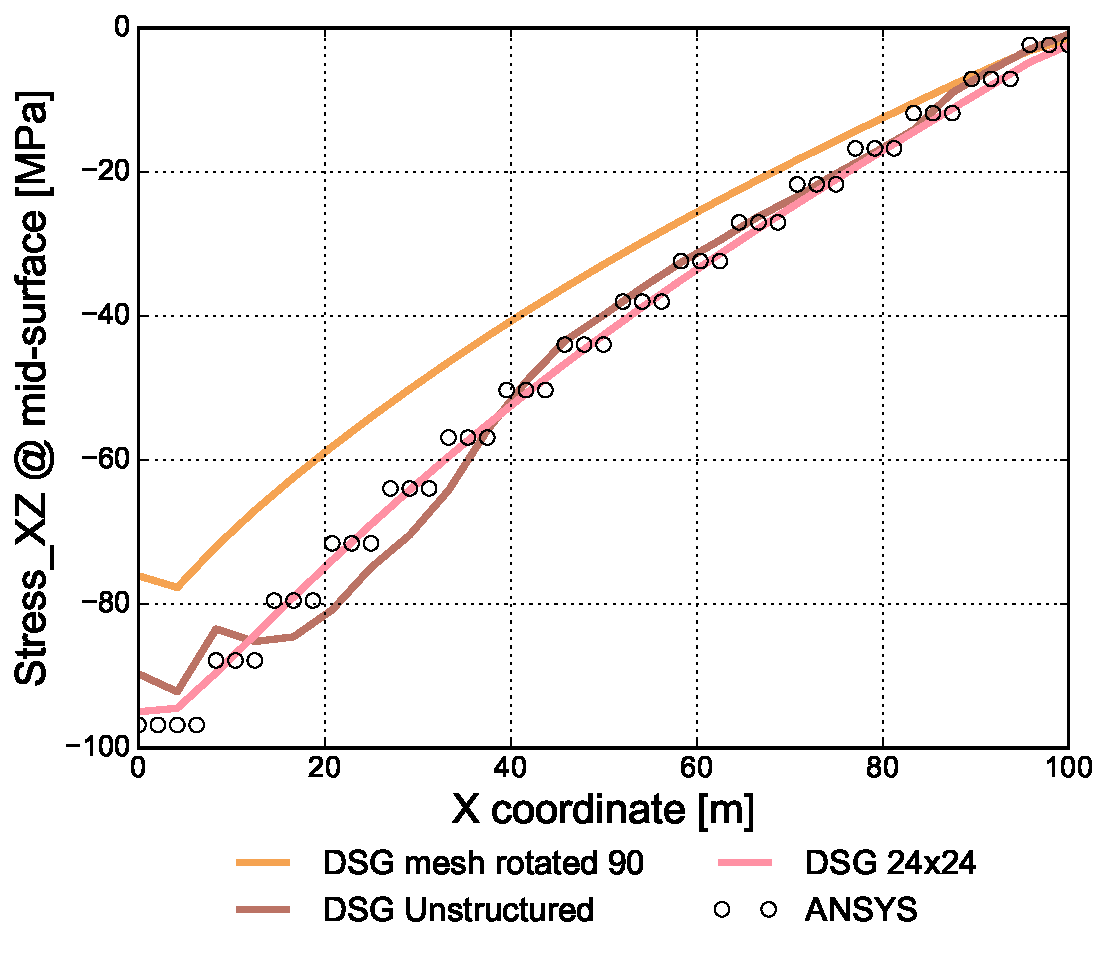
\includegraphics[width=7.3cm]
		{images/navier_plate_tri_s_xz.pdf}}
	\\
	\subfloat[Transverse shear stress (YZ) over Y coordinate]
	{\label{ref_label1}
		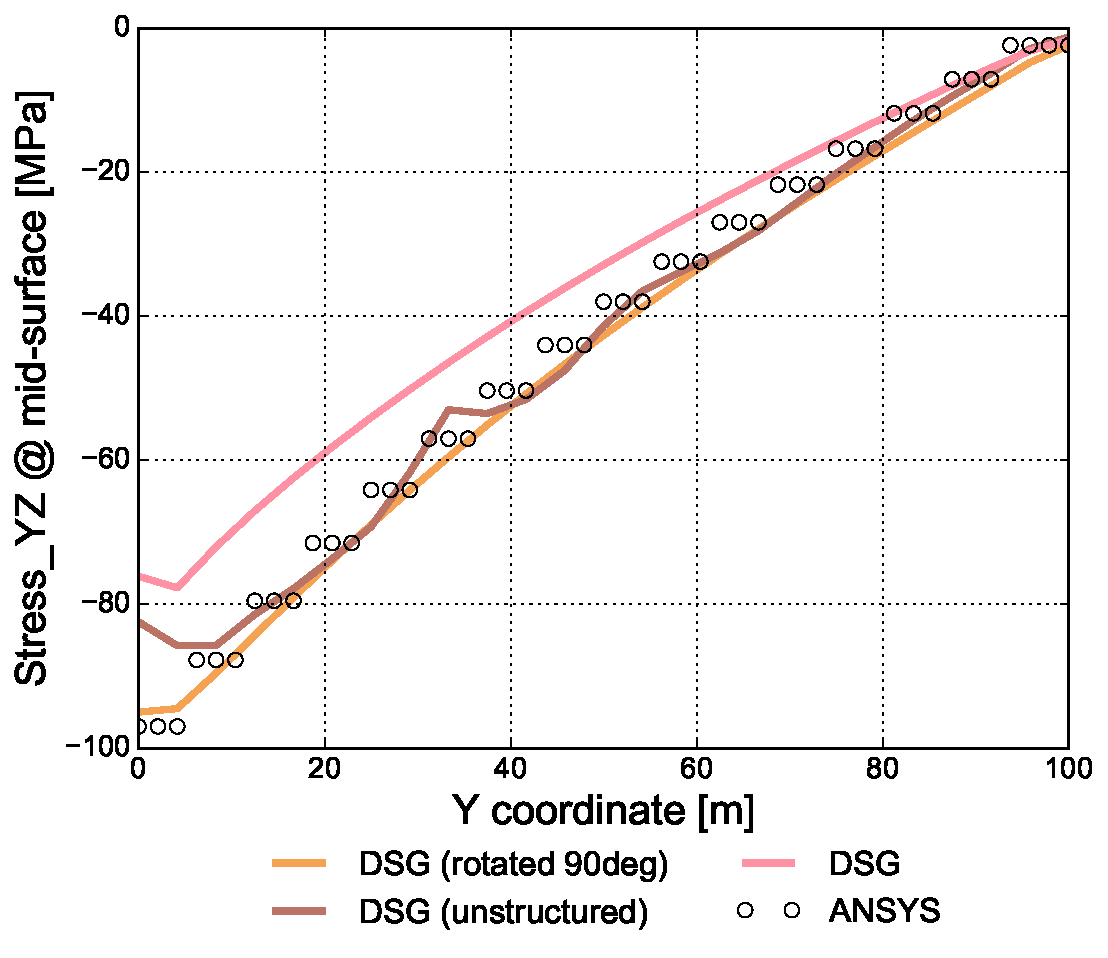
\includegraphics[width=7.3cm]
		{images/navier_plate_tri_s_yz.pdf}}
	\subfloat[Von Mises stress over plate diagonal]
	{\label{ref_label2}
		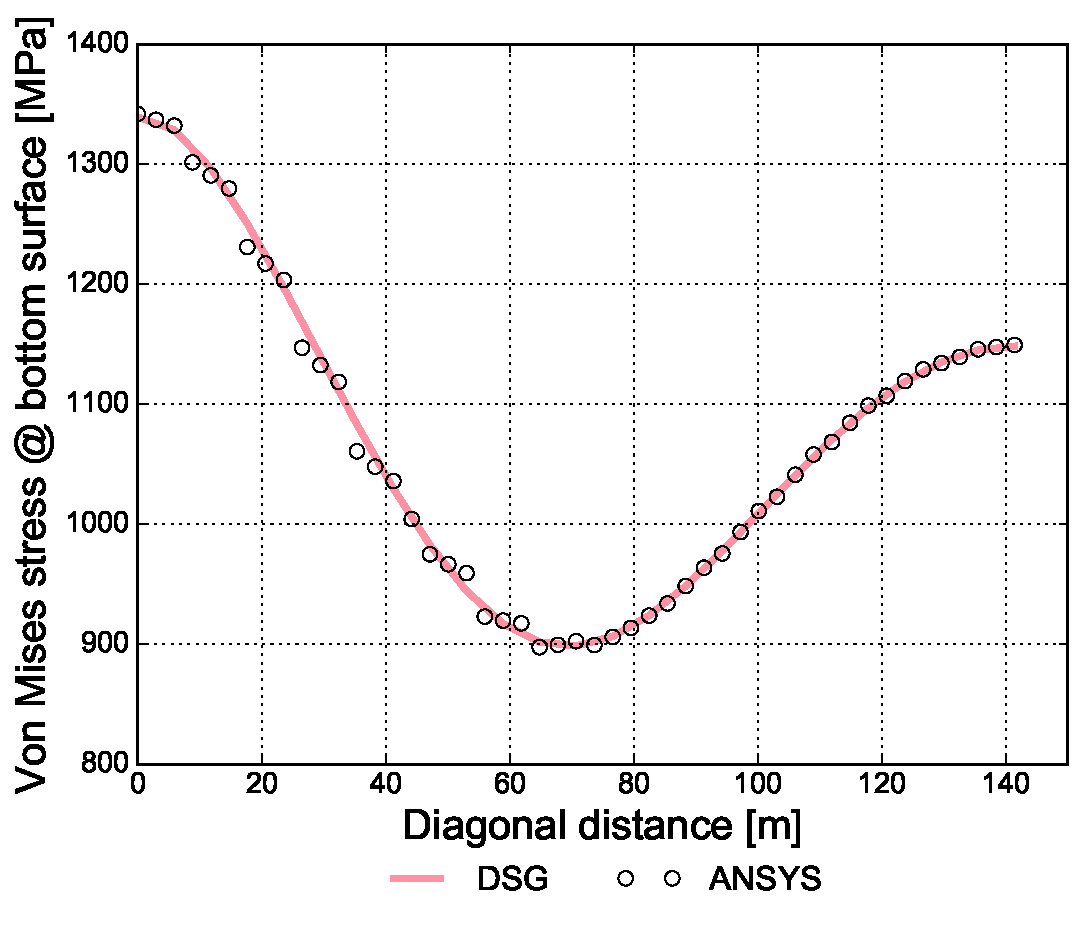
\includegraphics[width=7.3cm]
		{images/navier_plate_tri_vm.pdf}}
	\caption{\label{Navier_tri_s_xx_yy}Stresses of the Navier supported plate under uniformly distributed load}
\end{figure}

The DSG element shows good agreement with the ANSYS results across all stress quantities considered.

\section{Composite tests}

The extension of both shell elements to handle composite laminates requires it's own validation across the range of tests considered for isotropic shells. The following tests consider the performance of both elements in cases which all employ composite materials. As per the preceding isotropic element tests, cases across linear/non-linear statics, linear/non-linear dynamics, and quantity recovery are examined.

\subsection{Composite linear statics: composite barrel vault}
\label{validation:composite barrel vault}
The composite barrel vault is an extension of the Scordelis-Lo roof obstacle course test to composite materials \cite{reddy2004mechanics}. Corresponding to the following figure, the problem is defined with: $\alpha = 40^{\circ},\ R = 300,\ a = 600$ and $q = 0.625$. The reference quantity is the vertical displacement at the centre of the roof (point A).

\begin{figure}[H]
	\centering
	\def\svgwidth{\columnwidth}
	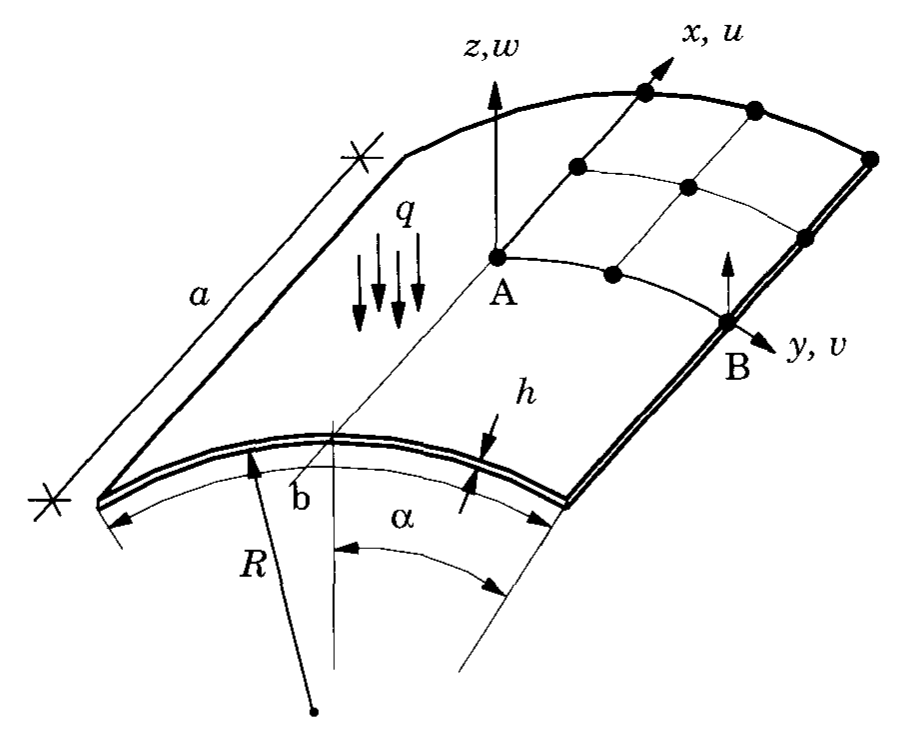
\includegraphics[width=7.3cm]{images/composite_barrel_vault_def.png}
	\caption{Definition of the composite barrel vault test \cite{reddy2004mechanics}}
\end{figure}

The composite material is considered with cross-ply [0/90/0/90...] and angle-ply [-45/45/-45/45/...] lamina stacking arrangements, with each ply having the following material properties: $E_1 = 25 E_2,\ E_2 = 1.2 \times 10^5,\ G_{12} = G_{13} = 0.5 E_2,\ G_{23} = 0.2 E_2$ and $\nu_{12} = 0.25$. Furthermore, the tests are carried out over slenderness ratios of $S = \frac{R}{h} = 20,\ 50,\ 100$ which correspond to total laminate thicknesses of $h = 15,\ 6,\ 3$.

\begin{figure}[H]
	\subfloat[2 ply cross layup]
	{\label{ref_label1}
		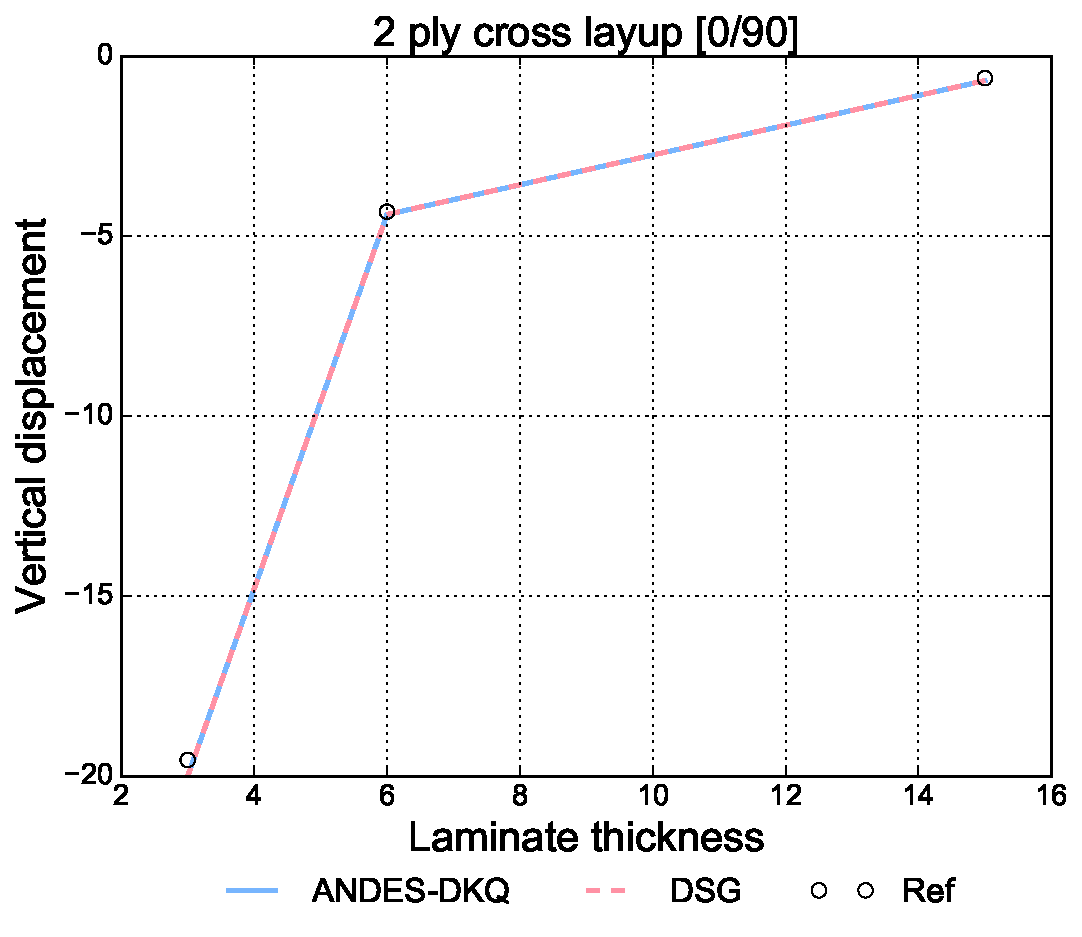
\includegraphics[width=7.3cm]
		{images/cross2ply.pdf}}
	\subfloat[10 ply cross layup]
	{\label{ref_label2}
		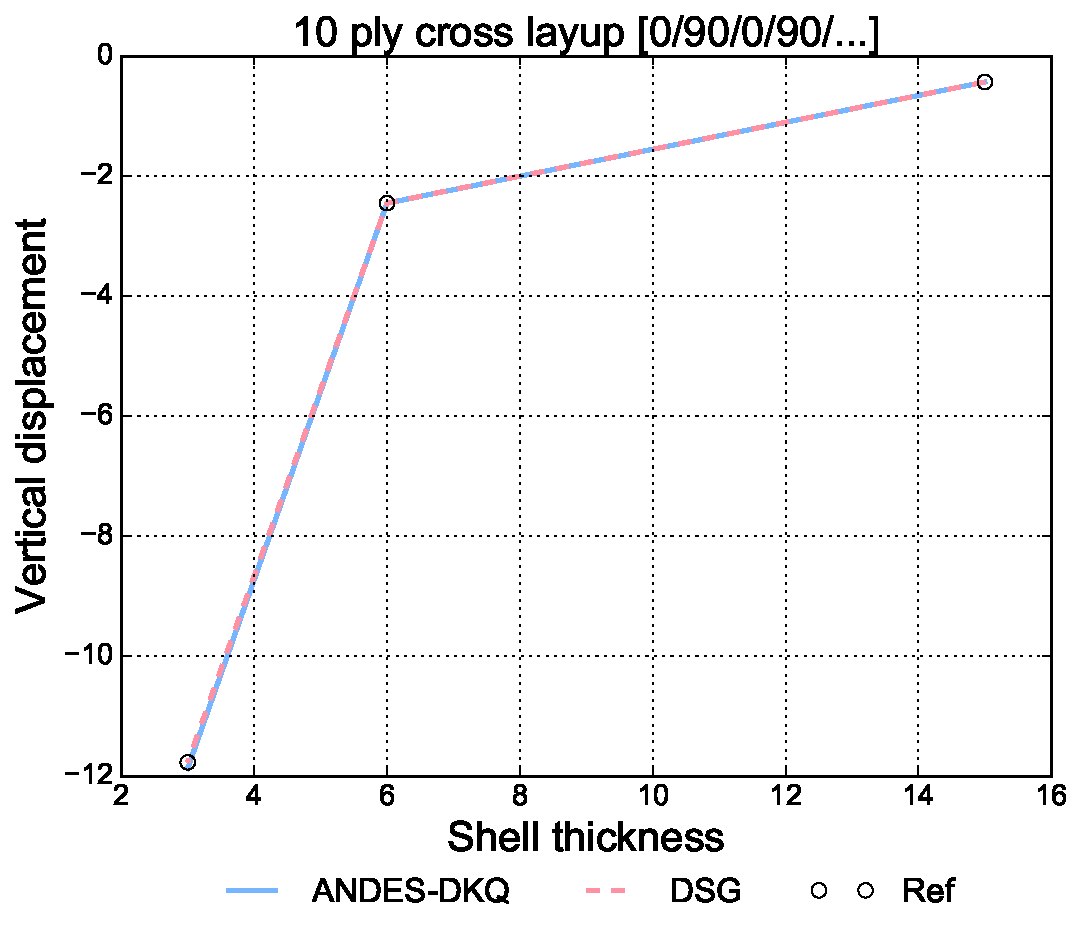
\includegraphics[width=7.3cm]
		{cross10ply.pdf}}
	\\
	\subfloat[2 ply angle layup]
	{\label{ref_label1}
		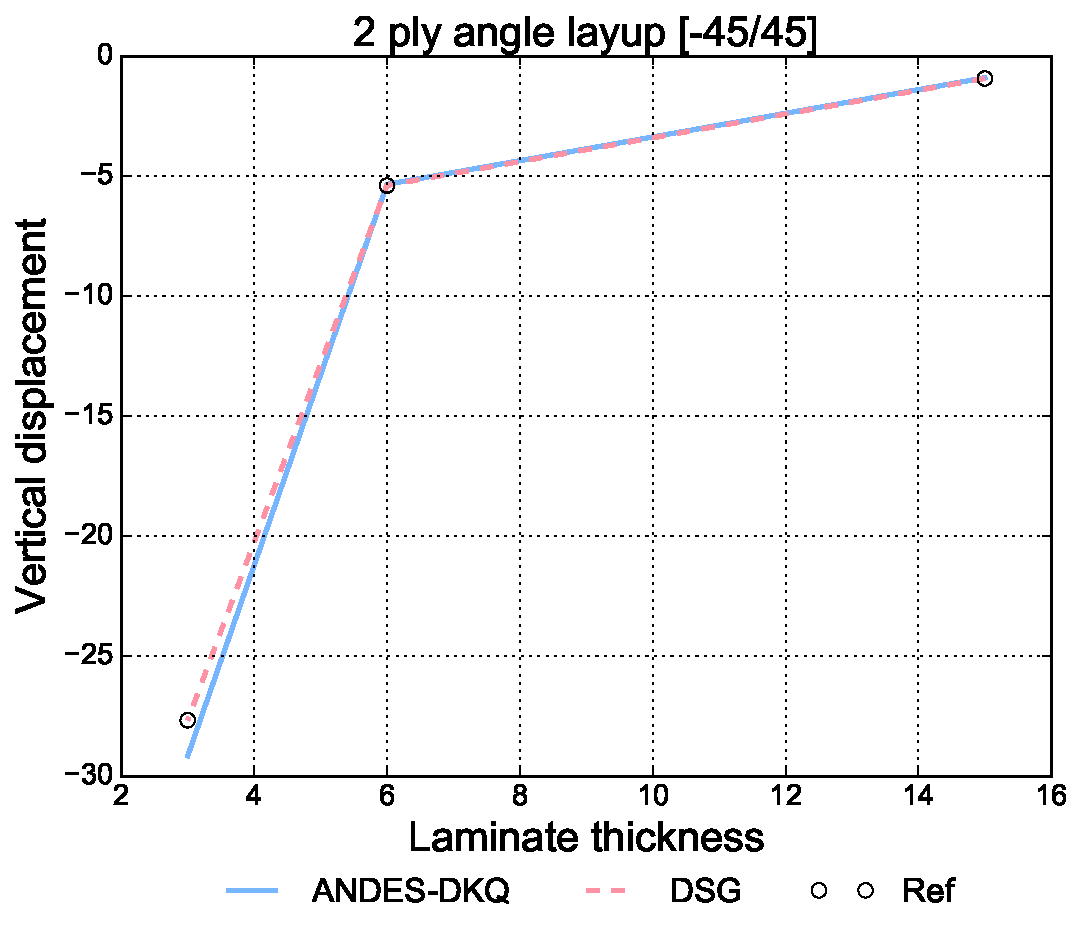
\includegraphics[width=7.3cm]
		{images/angle2ply.pdf}}
	\subfloat[10 ply angle layup]
	{\label{ref_label2}
		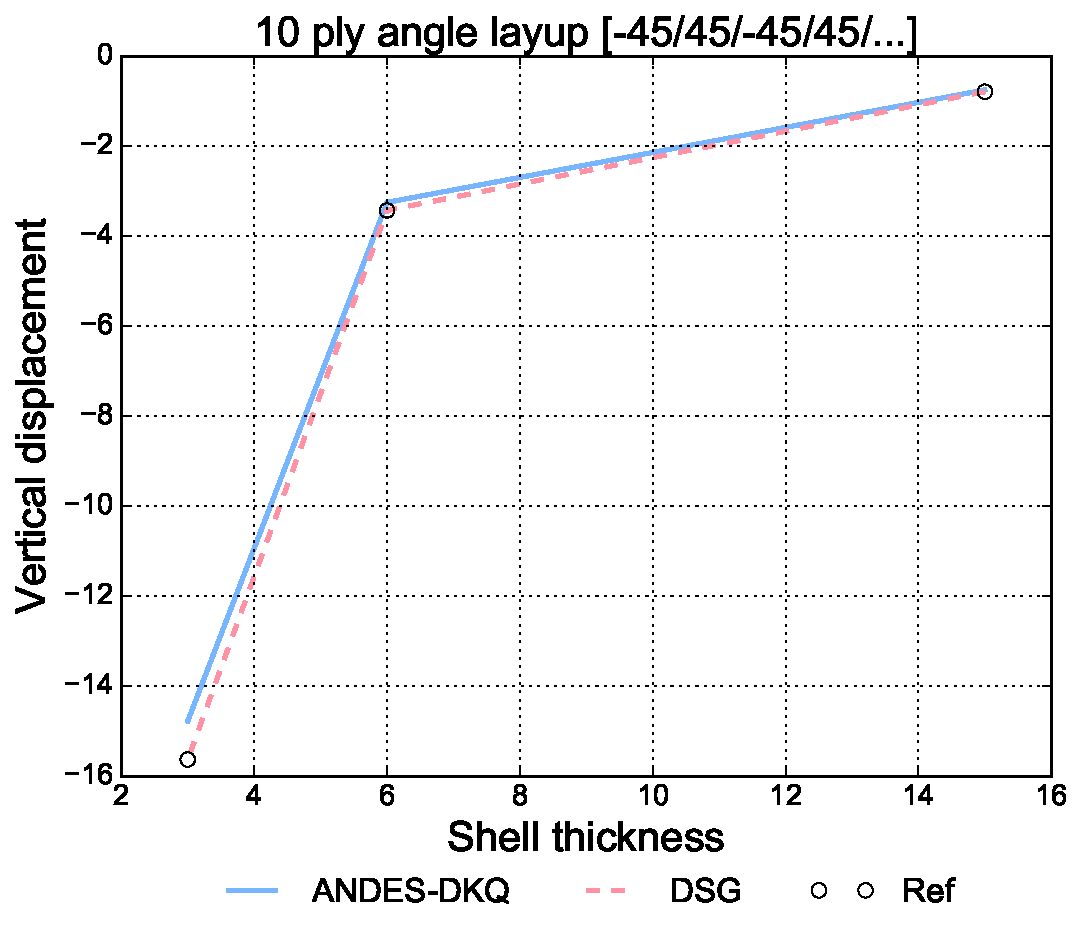
\includegraphics[width=7.3cm]
		{images/angle10ply.pdf}}
\caption{\label{Composite barrel vault benchmark: cross layup}Composite barrel vault test results}
\end{figure}

%\begin{figure}[H]
%	\subfloat[2 ply angle layup]
%	{\label{ref_label1}
%		\includegraphics[width=7.3cm]
%		{images/angle2ply.pdf}}
%	\subfloat[10 ply angle layup]
%	{\label{ref_label2}
%		\includegraphics[width=7.3cm]
%		{images/angle10ply.pdf}}
%	\caption{\label{Composite barrel vault benchmark: angle layup}Composite barrel vault benchmark: angle layup}
%\end{figure}

Across the wide range of testing considered both elements exhibit excellent agreement with the reference solution. The ANDES-DKQ element performance slightly deteriorates in the thin angle layup scenarios, however, the result is still quite accurate.

\subsection{Composite linear static: clamped cylinder}

Another test for the composite shell elements in the realm of linear statics is a cylinder clamped at both ends subject to internal pressure. A cylinder of length $a = 20$, radius $R = 20$ and total laminate thickness of $h = 1$ is subject to a uniform internal pressure of $p_0 = \frac{6410}{\pi}$ \cite{reddy2004mechanics}. The key quantity of interest is the maximum radial displacement of the cylinder, with the reference solution taken from Reference \cite{reddy2004mechanics}.

\begin{figure}[H]
	\centering
	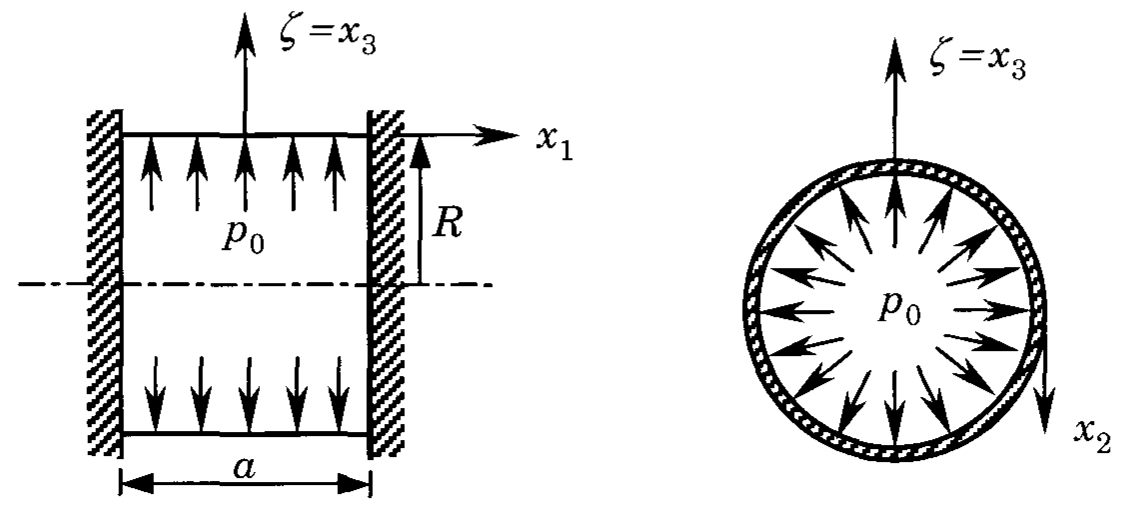
\includegraphics[width=12cm]{images/composite_clamped_cylinder_def.png}
	\caption{Composite clamped cylinder test definition}
	\label{fig:composite_clamped_cyl_def}
\end{figure}

The laminate is considered in both single and double layer arrangements, with the lamina properties defined as: $E_1 = 7.5\times10^6,\ E_2 = 2\times10^6,\ G_{12} = 1.25\times10^6,\ G_{13} = G_{23} = 0.625\times10^6$ and $\nu_{12} = 0.25$. Due to symmetry only half the cylinder was modelled, while the mesh was refined under the constraint of $circumferential\ divisions = 1.5\times axial\ divisions$.

\begin{figure}[H]
	\subfloat[1 ply layup]
	{\label{ref_label1}
		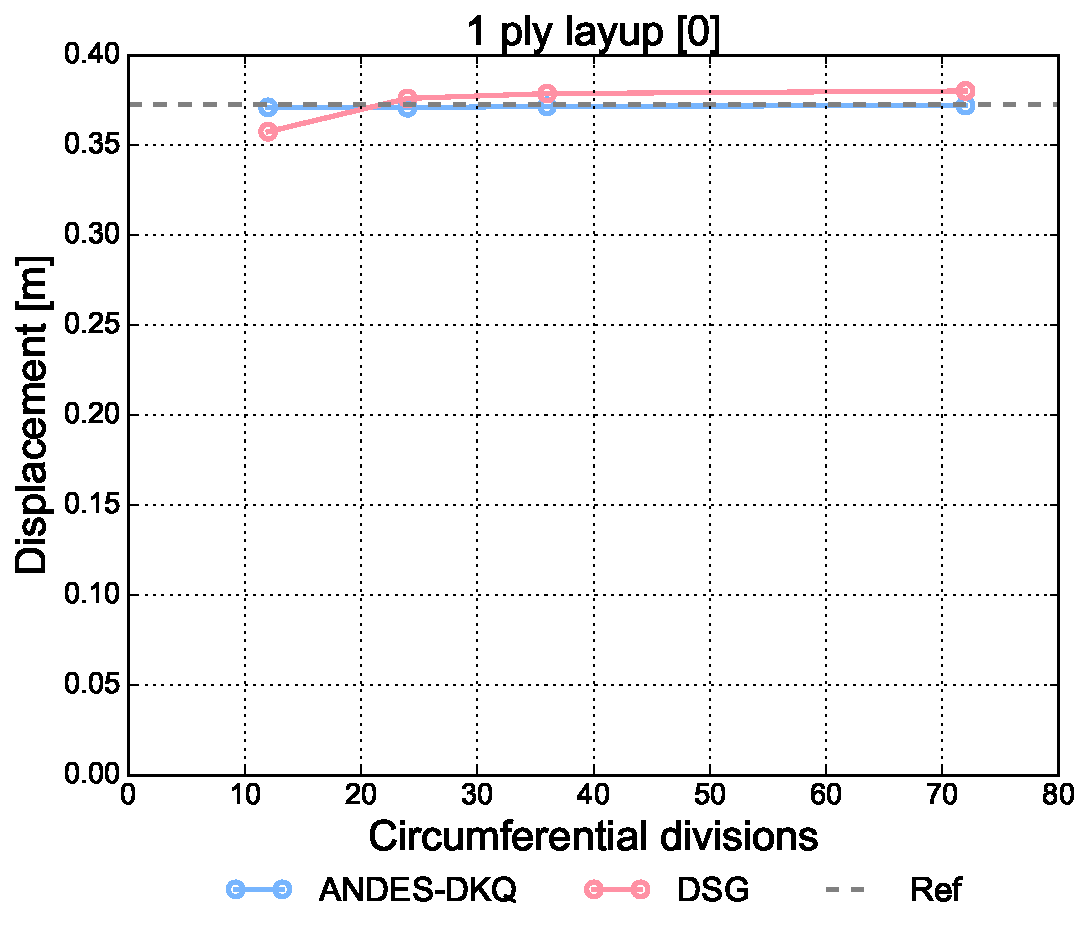
\includegraphics[width=7.3cm]
		{images/composite_clamped_cyl_0layup.pdf}}
	\subfloat[2 ply layup]
	{\label{ref_label2}
		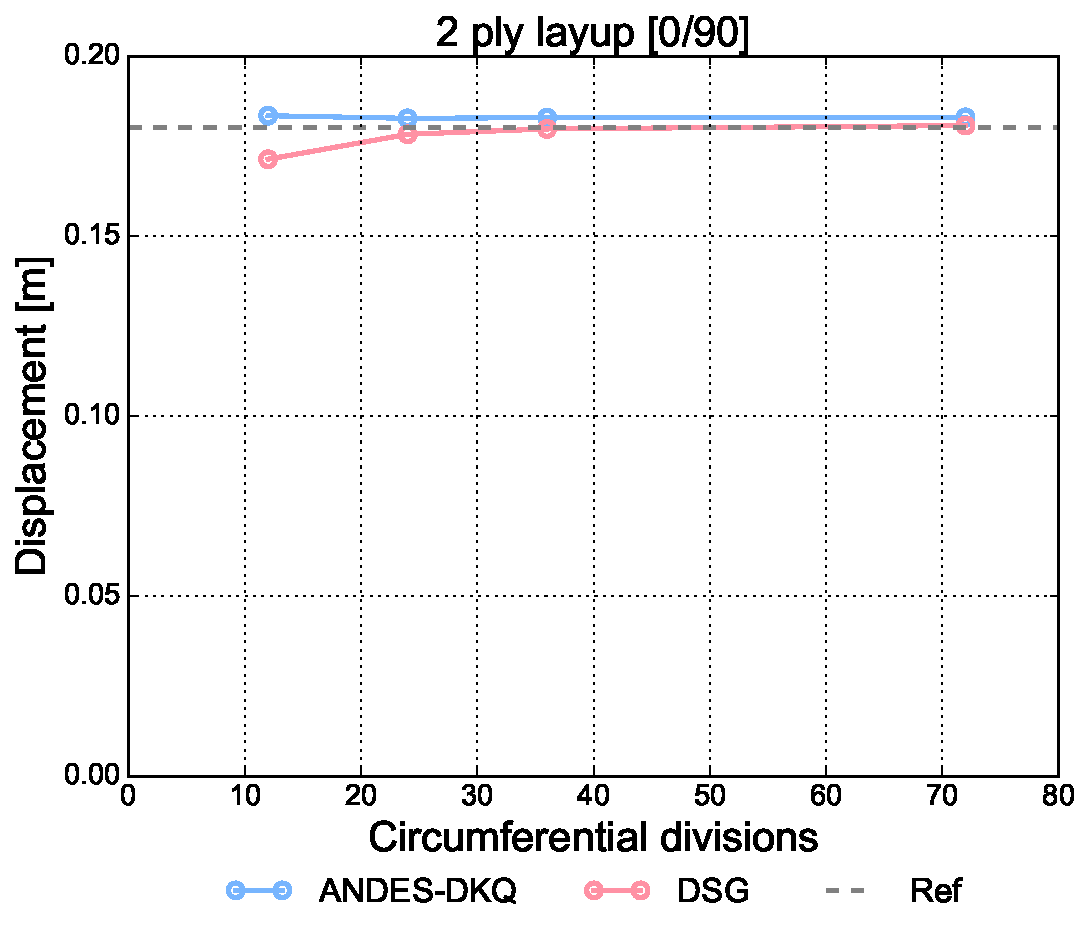
\includegraphics[width=7.3cm]
		{images/composite_clamped_cyl_090layup.pdf}}
	\caption{\label{Composite_clamped_cylinder_test}Composite clamped cylinder analysis convergence}
\end{figure}

Both elements quickly converge to the reference solution and maintain good performance as the mesh is refined further. The reference solution source \cite{reddy2004mechanics} notes that minor differences are expected between 3-parameter and 5-parameter shell models, however, the vagaries between the ANDES-DKQ and DSG elements are negligible compared to their excellent accuracy.

\subsection{Composite non-linear static: composite hinged cylindrical roof}

To consider the non-linear static performance of composite shells, the hinged cylindrical roof test in section \ref{validation:hinged cyl roof} is identically repeated with a laminate material. The composite laminate of total thickness $h = 12.7mm$ is composed of laminae with properties $E_1 = 3.3\times10^9,\ 1.1\times10^9,\ G_{12} = G_{13} = G_{23} = 0.66\times10^9$ and $\nu_{12} = 0.25$ arranged in a [90/0/90] stacking sequence \cite{Sze2004}.

\begin{figure}[H]
	%\centering
	\subfloat[Composite hinged cylindrical roof definition \cite{Sze2004}]
	{\label{ref_label1}
		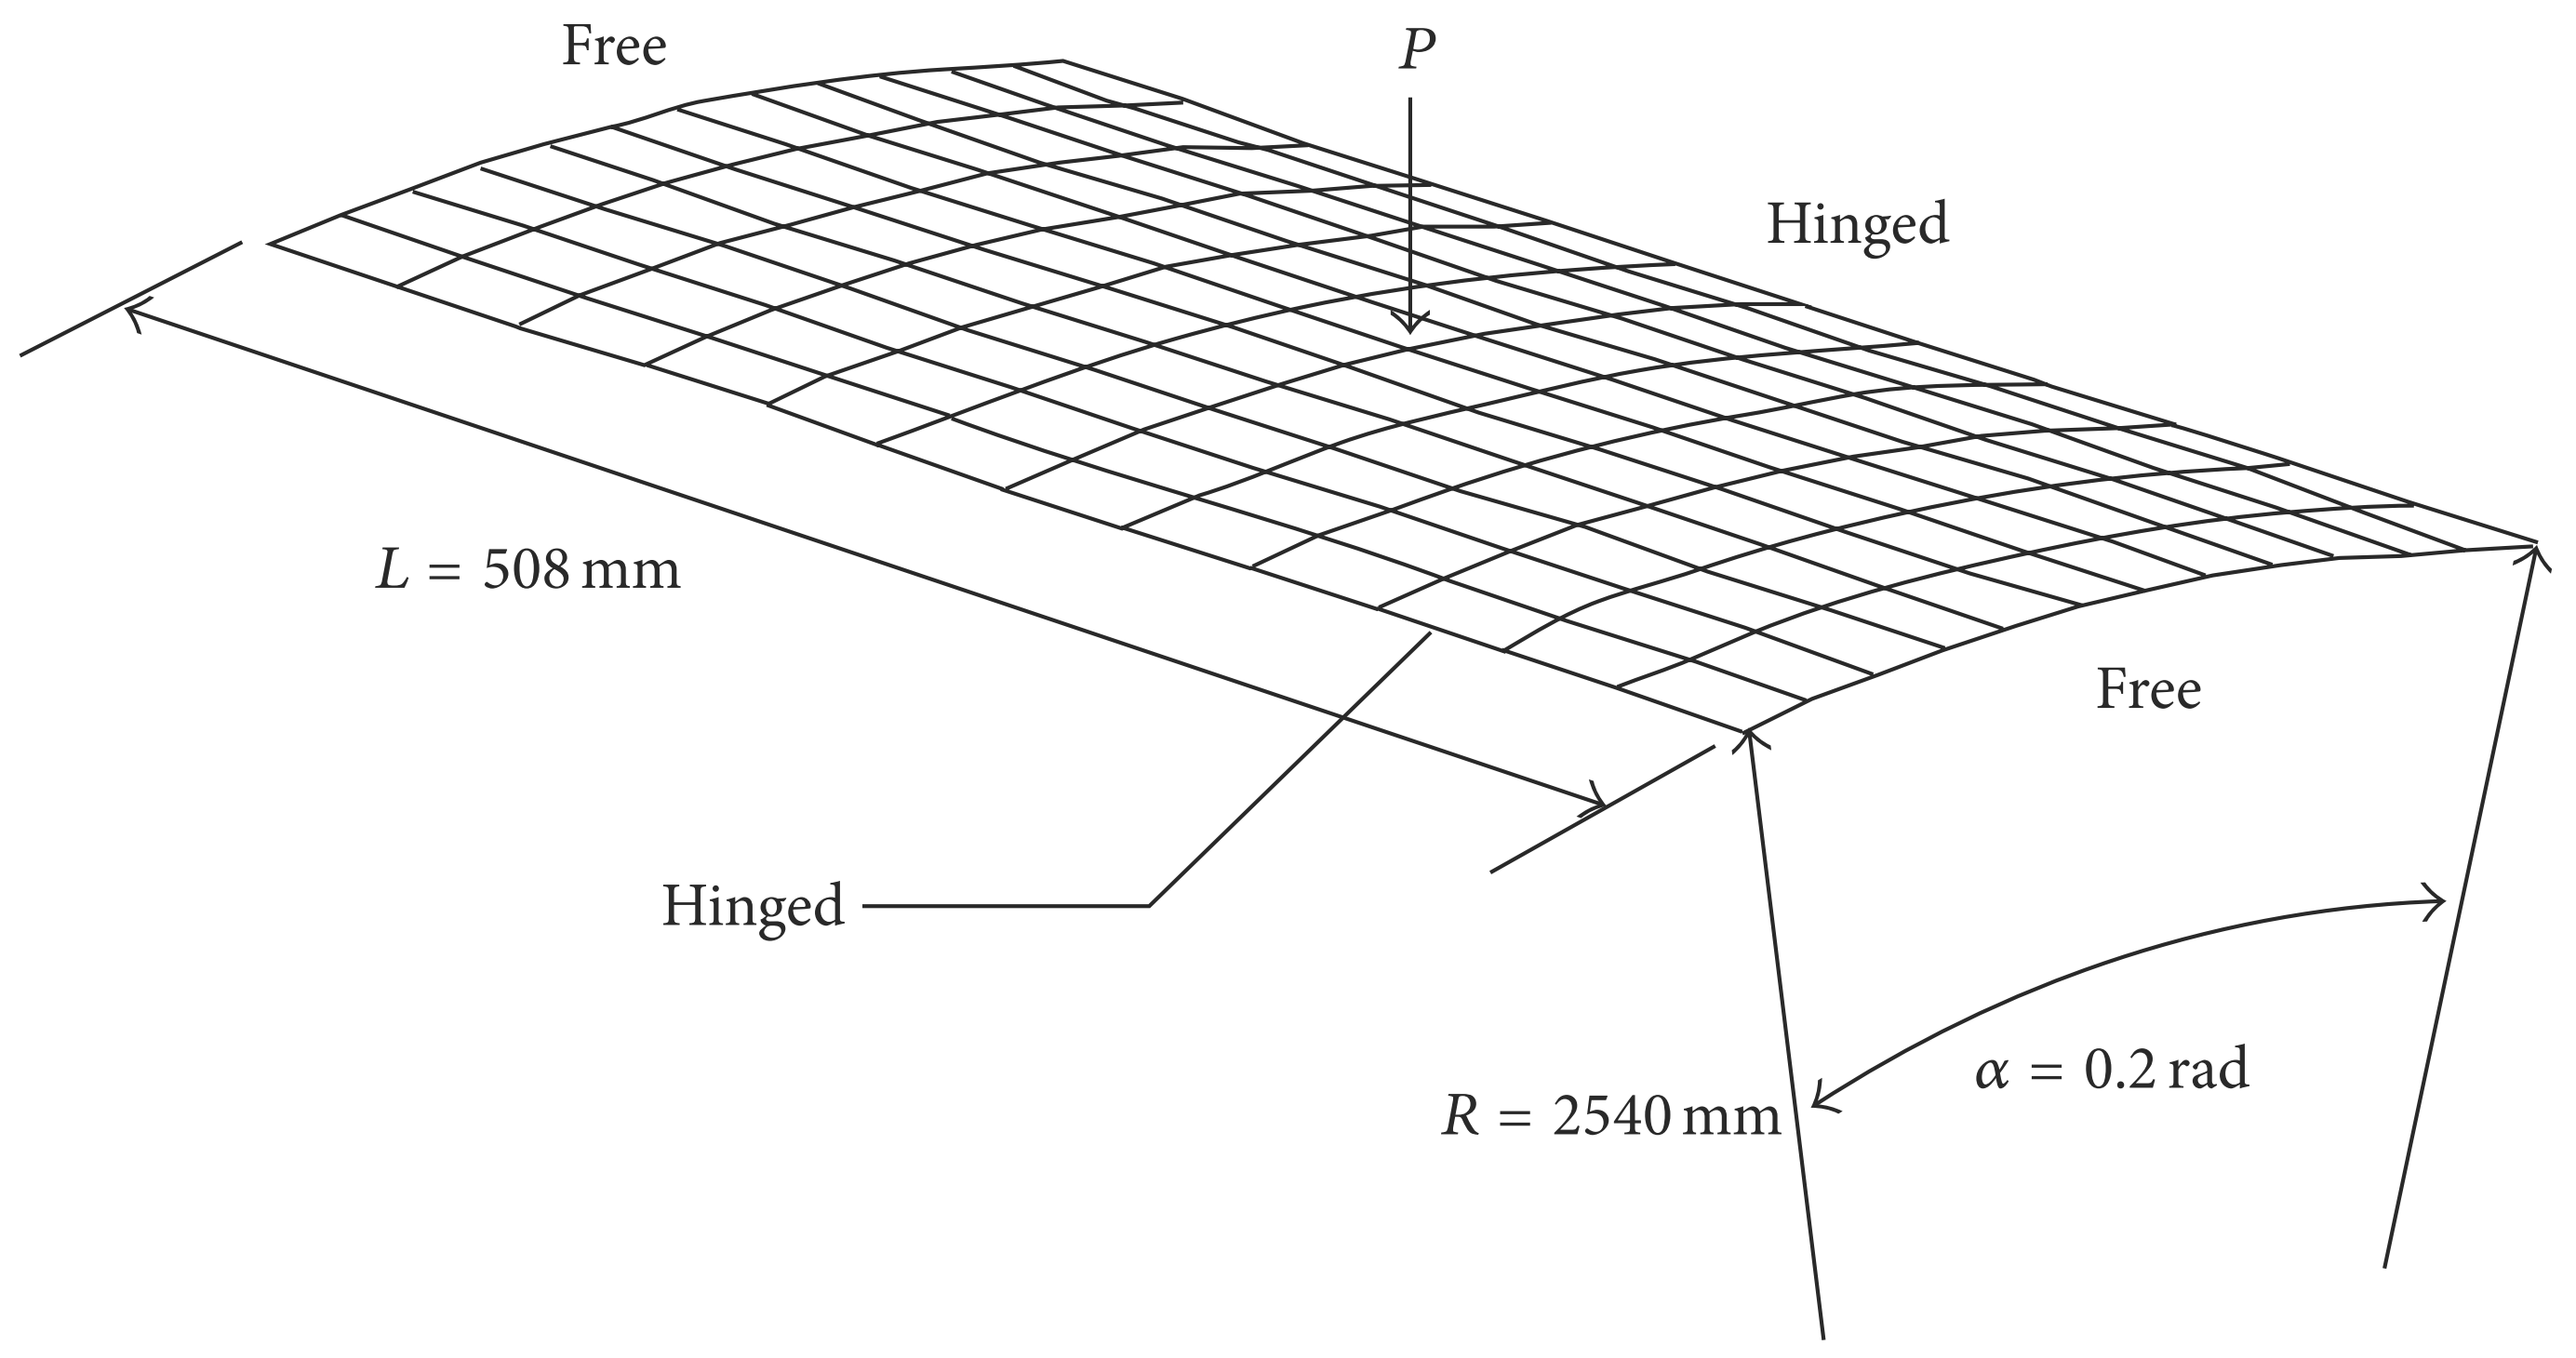
\includegraphics[width=7.3cm]
		{images/hinged_cylindrical_roof.png}}
	\subfloat[Load-displacement curve of composite hinged cylindrical roof]
	{\label{ref_label2}
		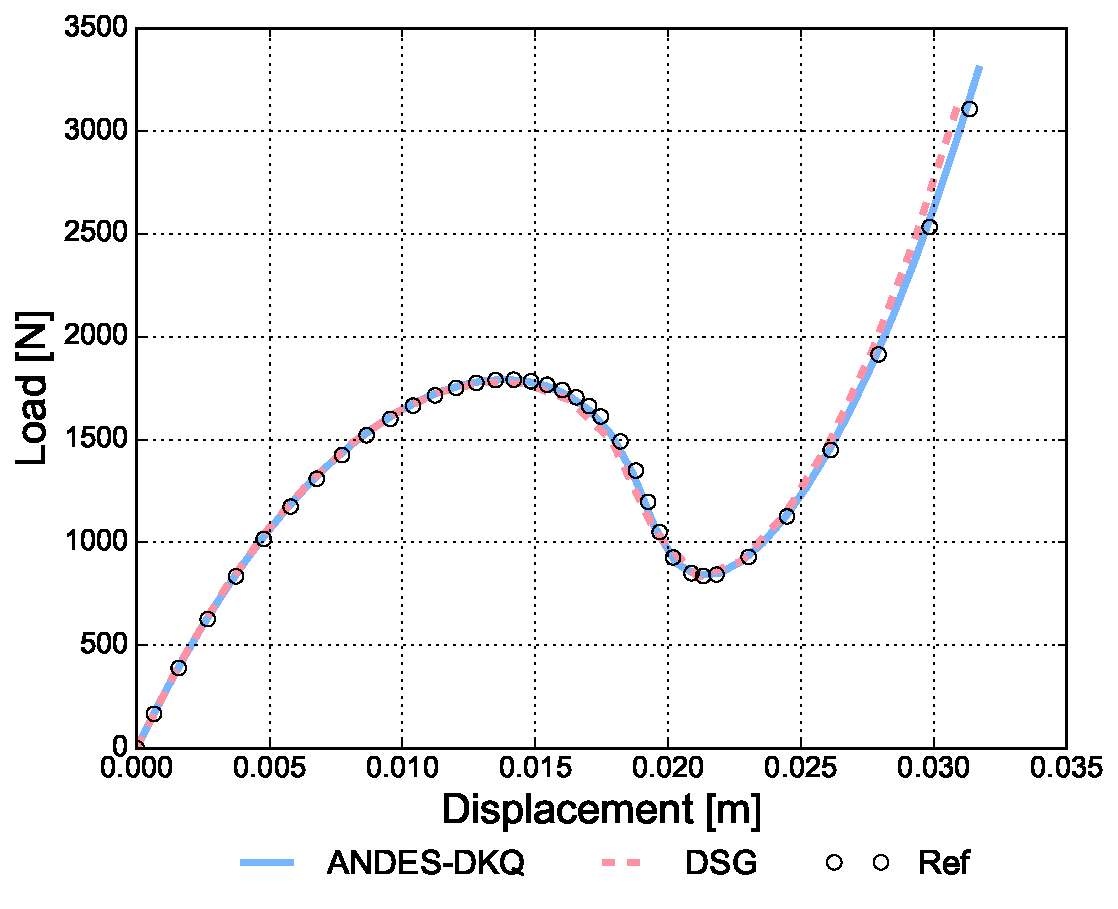
\includegraphics[width=7.3cm]
		{images/Load_displacement_curve_composite_hinged_cylindrical_roof.pdf}}
	\caption{\label{ref_label_overall}Composite hinged cylindrical roof test}
\end{figure}

The load displacement curve above clearly shows the ability of both elements to accurately resolve the equilibrium path of the composite roof through the pre and post-critical ranges.

\subsection{Composite dynamics: shell pendulum and oscillating square plate - FIXUP SECOND GRAPH FONT SIZE}

The shell pendulum test originally presented in section \ref{validation:shell pendulum} is identically repeated for a composite laminate material. A laminate of total thickness $h = 0.1m$ is considered with a stacking sequence of [0/90/90/0]. The material properties of each lamina are as per those defined in the composite barrel vault test (section \ref{validation:composite barrel vault}). Since the general lumped and consistent mass matrices were verified in section \ref{validation:shell pendulum}, only the lumped case is considered in in this test to validate the correct integration of composite material in dynamics. The reference solution for this test is that obtained by Strand7 with a lumped mass matrix.
%swinging plate material setup:
%	SHELL_ORTHOTROPIC_LAYERS  [4,9] (
%(0.025,0,7.85E+03,3.00E+09,1.20E+08,2.50E-01,6.00E+07,6.00E+07,2.40E+07),
%(0.025,90,7.85E+03,3.00E+09,1.20E+08,2.50E-01,6.00E+07,6.00E+07,2.40E+07),
%(0.025,90,7.85E+03,3.00E+09,1.20E+08,2.50E-01,6.00E+07,6.00E+07,2.40E+07),
%(0.025,0,7.85E+03,3.00E+09,1.20E+08,2.50E-01,6.00E+07,6.00E+07,2.40E+07)
%)

A second composite dynamic test considers the square Navier supported plate described in section \ref{validation:DSG navier unifom} subject to a uniform transverse pressure of $q = 1$. The material is changed from an isotropic material to a $h = 2$ thick laminate of layup $[0/90]_4$. The lamina properties are as per those defined in section \ref{validation:composite barrel vault} with the exception of $\rho = 1000$. The reference solution for this test is that obtained by Strand7 with a lumped mass matrix.
%vibrating square material setup:
%	SHELL_ORTHOTROPIC_LAYERS  [8,9] (
%(0.25,0,1000,3.00E+08,1.20E+07,2.50E-01,6.00E+06,6.00E+06,2.40E+06),
%(0.25,90,1000,3.00E+08,1.20E+07,2.50E-01,6.00E+06,6.00E+06,2.40E+06),
%(0.25,0,1000,3.00E+08,1.20E+07,2.50E-01,6.00E+06,6.00E+06,2.40E+06),
%(0.25,90,1000,3.00E+08,1.20E+07,2.50E-01,6.00E+06,6.00E+06,2.40E+06),
%(0.25,0,1000,3.00E+08,1.20E+07,2.50E-01,6.00E+06,6.00E+06,2.40E+06),
%(0.25,90,1000,3.00E+08,1.20E+07,2.50E-01,6.00E+06,6.00E+06,2.40E+06),
%(0.25,0,1000,3.00E+08,1.20E+07,2.50E-01,6.00E+06,6.00E+06,2.40E+06),
%(0.25,90,1000,3.00E+08,1.20E+07,2.50E-01,6.00E+06,6.00E+06,2.40E+06)
%)

\begin{figure}[H]
	%\centering
	\subfloat[Vertical displacement over time for composite shell pendulum analysis]
	{\label{ref_label2}
		\includegraphics[width=7.3cm]
		{images/composite_shell_pendulum_lumped.pdf}}
	\subfloat[Vertical displacement over time for composite oscillating Navier square plate analysis]
	{\label{ref_label2}
		\includegraphics[width=7.3cm]
		{images/composite_vibrating_square.pdf}}
	\caption{\label{Composite dynamic benchmarks}Composite dynamic tests}
\end{figure}

As per the isotropic dynamic tests, the composite tests agree very well with the reference Strand7 solutions. Figure \ref{Composite dynamic benchmarks}(b) reveals that the DSG element slightly deviates as the simulated time accumulates, however, the error in period is less than 1.3\%.

\subsection{Composite stress recovery: tensile test}
The first test to interrogate the stress recovery accuracy of the composite shell elements is a relatively simple tensile test \cite{nasanettles1994}. A horizontal rectangular tensile test token of $10\times2\times0.02$ total thickness is clamped at one end while the other end is subject to a tensile load of 1000. The token laminate layup is [0/90/90/0] while the material properties of each lamina are defined as: $E_1 = 200.1\times10^5,\ E_2 = 130.1\times10^4,\ G_{12} = G_{13} = G_{23} = 100.1\times10^4$ and $\nu_{12} = 0.3$. Results of the analysis are taken from the mid-length $(x=5)$ of the test token and are averaged across the width. The reference solution for the stresses is from Reference \cite{nasanettles1994} with a Strand7 analysis of the problem providing the Tsai-Wu reference. 
%Example from Nasa composite doc, example 3. Tensile test token was 10x2x0.02 total thickness. Layup was [0,45,45,0].
%Reference tsai-wu results are "Modified tsai-wu" of the same problem on Strand7 FEA software.
%Material was :
%(0.005,0,7850,20010000,1301000,0.3,1001000,1001000,1001000,80000,50000,4000,30000,6000,6000,6000).

\begin{figure}[H]
	%\centering
	\subfloat[Normal stress (XX) throughout thickness]
	{\label{ref_label1}
		\includegraphics[width=7.3cm]
		{images/nasa3_thru_s_xx.pdf}}
	\subfloat[Normal stress (YY) throughout thickness]
	{\label{ref_label2}
		\includegraphics[width=7.3cm]
		{images/nasa3_thru_s_yy.pdf}}
	\\
	\subfloat[In plane shear stress strain (XY) throughout thickness]
	{\label{ref_label1}
		\includegraphics[width=7.3cm]
		{images/nasa3_thru_s_xy.pdf}}
	\subfloat[Tsai-Wu reserve factor throughout thickness]
	{\label{ref_label2}
		\includegraphics[width=7.3cm]
		{images/nasa3_thru_tsai.pdf}}
	\caption{\label{Nasa3_stresses}Stresses and Tsai-Wu results of the composite tensile test}
\end{figure}

The four figures above, illustrating various stresses and Tsai-Wu reserve factor throughout the laminate thickness, confirm the accurate stress recovery of both elements. Although the recovery of Stress\_YY may initially not seem as accurate as the others, it's scale is 3 orders of magnitude less than the primary stress mode Stress\_XX. It's expected with stress values so low that much of this acceptable deviation is due to rounding errors, both in the implemented elements and the reference literature itself. The Tsai-Wu reserve factor results of both elements are in excellent agreement with the reference values.

\subsection{Composite stress recovery: Navier supported laminate under sinusoidal load}
The second composite stress recovery test considers the bending dominated scenario of a Navier supported square laminate subject to a sinusoidal load \cite{reddy2004mechanics}. As per the isotropic stress recovery testing, separate tests were carried out for the two elements: the ANDES-DKQ composite test is based off of section \ref{validation:navier plate under sinusoidal load} and the DSG from section \ref{validation:DSG navier unifom}. Both analyses have a transverse sinusoidally distributed transverse pressure defined as $q = -100 sin(\frac{x\pi}{200})sin(\frac{y\pi}{200})$ and consider a $h = 10$ thick [0/90/90/0] laminate with individual lamina properties as per those defined in \ref{validation:composite barrel vault}.

The reference solutions are taken from Reference \cite{reddy2004mechanics}, with the ANDES-DKQ element compared to a classical plate theory solution and the DSG element compared to a Navier plate closed form solution. As per the reference solutions, results for different quantities are sampled at different positions in the square plate. Referring to figure \ref{validation:pic navier plate} (repeated below for clarity), the stress and strains are recovered throughout the thickness of the laminate at the following positions:
\begin{align*} 
\sigma_{xx} = \sigma_{xx}(\frac{a}{2},\ \frac{b}{2},\ z)
\hspace{10mm}
\epsilon_{xx} = \epsilon_{xx}(\frac{a}{2},\ \frac{b}{2},\ z)
\\
\sigma_{yy} = \sigma_{yy}(\frac{a}{2},\ \frac{b}{2},\ z)
\hspace{10mm}
\epsilon_{yy} = \epsilon_{yy}(\frac{a}{2},\ \frac{b}{2},\ z)
\\
\sigma_{xy} = \sigma_{xy}(0,\ 0,\ z)
\hspace{10mm}
\epsilon_{xy} = \epsilon_{xy}(0,\ 0,\ z)
\\
\sigma_{xz} = \sigma_{xz}(0,\ \frac{b}{2},\ z)
\hspace{10mm}
\epsilon_{xz} = \epsilon_{xz}(0,\ \frac{b}{2},\ z)
\\
\sigma_{yz} = \sigma_{yz}(\frac{a}{2},\ 0,\ z)
\hspace{10mm}
\epsilon_{yz} = \epsilon_{yz}(\frac{a}{2},\ 0,\ z)
%\label{eqs val comp stress}
\end{align*}
\begin{figure}[H]
	\centering
	\def\svgwidth{\columnwidth}
	\includegraphics[width=7.3cm]{images/navier_plate_def.png}
	%\caption{Definition of the Navier supported plate test \cite{reddy2004mechanics}}
	%\label{validation:pic navier plate2}
\end{figure}

The following set of graphs illustrate the results of the ANDES-DKQ element compared with the reference classical plate theory solution.
%\begin{equation} 
%\sigma_{xx} = \sigma_{xx}(\frac{a}{2},\ \frac{b}{2},\ z)
%\label{eqs val comp stress}
%\end{equation}

%Ref is Reddy p527 table 9.3.2. 200x200x10 total thickness. 
\begin{figure}[H]
	%\centering
	\subfloat[Normal strain (XX) throughout thickness]
	{\label{ref_label1}
		\includegraphics[width=7.3cm]
		{images/navier_plate_composite_quad_e_xx.pdf}}
	\subfloat[Normal stress (XX) throughout thickness]
	{\label{ref_label2}
		\includegraphics[width=7.3cm]
		{images/navier_plate_composite_quad_s_xx.pdf}}
	\\
	\subfloat[Normal strain (YY) throughout thickness]
	{\label{ref_label1}
		\includegraphics[width=7.3cm]
		{images/navier_plate_composite_quad_e_yy.pdf}}
	\subfloat[Normal stress (YY) throughout thickness]
	{\label{ref_label2}
		\includegraphics[width=7.3cm]
		{images/navier_plate_composite_quad_s_yy.pdf}}
	\\
	\subfloat[In plane shear strain (XY) throughout thickness]
	{\label{ref_label1}
		\includegraphics[width=7.3cm]
		{images/navier_plate_composite_quad_e_xy.pdf}}
	\subfloat[In plane shear stress (XY) throughout thickness]
	{\label{ref_label2}
		\includegraphics[width=7.3cm]
		{images/navier_plate_composite_quad_s_xy.pdf}}
	\caption{\label{Navier_quad_composite_s_xx_yy}Stresses and strains of the Navier supported ANDES-DKQ laminate under a sinusoidally distributed load}
\end{figure}

The following set of graphs compare the DSG element results with those of the reference closed form solution.

\begin{figure}[H]
	%\centering
	\subfloat[Normal strain (XX) throughout thickness]
	{\label{ref_label1}
		\includegraphics[width=7.3cm]
		{images/navier_plate_composite_tri_e_xx.pdf}}
	\subfloat[Normal stress (XX) throughout thickness]
	{\label{ref_label2}
		\includegraphics[width=7.3cm]
		{images/navier_plate_composite_tri_s_xx.pdf}}
	\\
	\subfloat[Normal strain (YY) throughout thickness]
	{\label{ref_label1}
		\includegraphics[width=7.3cm]
		{images/navier_plate_composite_tri_e_yy.pdf}}
	\subfloat[Normal stress (YY) throughout thickness]
	{\label{ref_label2}
		\includegraphics[width=7.3cm]
		{images/navier_plate_composite_tri_s_yy.pdf}}
	\\
	\subfloat[In plane shear strain (XY) throughout thickness]
	{\label{ref_label1}
		\includegraphics[width=7.3cm]
		{images/navier_plate_composite_tri_e_xy.pdf}}
	\subfloat[In plane shear stress (XY) throughout thickness]
	{\label{ref_label2}
		\includegraphics[width=7.3cm]
		{images/navier_plate_composite_tri_s_xy.pdf}}
	\caption{\label{Navier_tri_composite_s_xx_yy}In plane stresses and strains of the Navier supported DSG laminate under a sinusoidally distributed load}
\end{figure}

\begin{figure}[H]
	%\centering
	\subfloat[Transverse shear strain (XZ) throughout thickness]
	{\label{ref_label1}
		\includegraphics[width=7.3cm]
		{images/navier_plate_composite_tri_e_xz.pdf}}
	\subfloat[Transverse shear stress (XZ) throughout thickness]
	{\label{ref_label2}
		\includegraphics[width=7.3cm]
		{images/navier_plate_composite_tri_s_xz.pdf}}
	\\
	\subfloat[Transverse shear strain (YZ) throughout thickness]
	{\label{ref_label1}
		\includegraphics[width=7.3cm]
		{images/navier_plate_composite_tri_e_yz.pdf}}
	\subfloat[Transverse shear stress (YZ) throughout thickness]
	{\label{ref_label2}
		\includegraphics[width=7.3cm]
		{images/navier_plate_composite_tri_s_yz.pdf}}
	\caption{\label{Navier_tri_composite_trans}Transverse shear stresses and strains of the Navier supported DSG laminate under a sinusoidally distributed load}
\end{figure}

The results of the ANDES-DKQ and DSG elements demonstrate the excellent composite stress recovery accuracy across all stresses considered. It also highlights the ability to resolve discontinuous stress distributions from smooth linear strains by considering properly rotated individual lamina material properties. As expected, the in-plane shear stresses (Stress\_XY) are smoothly linear because the in-plane shear modulus is invariant under planar rotation. The transverse shear stresses of the DSG are slightly less accurate than other stresses recovered, which is likely due to a combination of mild node-numbering dependency (as per the transverse shear stresses of section \ref{validation:DSG navier unifom}) and rounding having a pronounced effect on the comparatively low order-of-magnitude values.

In addition to the stresses and strains considered, the Tsai-Wu reserve factor was also calculated in the centre of the plate $(\frac{a}{2},\ \frac{b}{2},\ z)$ and compared against Tsai-Wu results from a Strand7 analysis of the problem. It must be noted that the Strand7 analysis software approximates the Tsai-Wu in-plane interaction coefficient $F_{12}$ (refer section \ref{tsai wu background}) as zero. Thus, to enable a proper comparison, results marked with an asterisk '*' have $F_{12} = 0$, while those without calculate $F_{12}$ as per equation \ref{eqscomp_tsai2}.

\begin{figure}[H]
	%\centering
	\subfloat[Tsai-Wu reserve factor throughout thickness of ANDES-DKQ element]
	{\label{ref_label1}
		\includegraphics[width=7.3cm]
		{images/navier_plate_composite_quad_tsai.pdf}}
	\subfloat[Tsai-Wu reserve factor throughout thickness of DSG element]
	{\label{ref_label2}
		\includegraphics[width=7.3cm]
		{images/navier_plate_composite_tri_tsai.pdf}}
	\caption{\label{Navier_tri_composite_trans}Tsai-Wu reserve factor through the thickness of the Navier supported DSG laminate under a sinusoidally distributed load}
\end{figure}

The figures above confirm accurate determination of the Tsai-Wu reserve factor in both elements. A central discontinuity is present in the ANDES-DKQ thin shell because it has no stress on the mid-plane under pure bending, yielding an infinite reserve factor. Focussing on the DSG element, the low magnitude of transverse shear stresses on the mid-plane yields a finite reserve factor of roughly 100, which has been omitted for clarity. These transverse shear stresses, which have a greater combined magnitude in the central laminae, are also the reason behind the small 'hooks' of lower reserve factors at the outer/inner ply boundaries.